% Chapter 5

\chapter{Results} % Main chapter title

\label{Results} % For referencing the chapter elsewhere, use \ref{Chapter1} 

\lhead{Chapter 5. \emph{Results}} % This is for the header on each page - perhaps a shortened title

This chapter presents the results of the methods described earlier in this thesis. The performance of the evolutionary methods used for the co-evolution of the morphology and the locomotion strategy of soft-robots is discussed. In the previous chapter, it has been shown how random generated soft-robot morphologies fail to produce any locomotion capabilities in this setting. Thus, the results obtained by these random methods are not discussed in this chapter. The performance of evolutionary methods is only presented. Pure novelty search is compared in respect to the goodness measure used in the simulations (displacement of soft-robots in body-lengths), with fitness-based search. The affect that novelty search has in the average and champion fitness of the population during the evolution is investigated in detail in the following sections. Additionally, both search methods are compared with respect to the number of novel behaviors they evolve during an evolution run. Moreover, the influence of the behavior metric in novelty search is shown, where all behavior metric proposed earlier are used to define the novelty of an individual. An altered number of closest behaviors in the sparsity equation of the novelty search, leads to an interesting conclusion about the effect it has in the evolution process. Genetic selection techniques such as competition and elitism are also used to improve the baseline methods. More specifically, elitism is used in a proposed methodology to incorporate fitness information in novelty search. Last, the performance of both methods are investigated within variant gravity levels. Showing that gravity conditions do not have an effect in favor of a specific search method. Furthermore, a discussion of evolved locomotion strategies under different gravity conditions shows how environmental conditions can affect the evolved morphologies and the strategies of soft-robots.

As in~\citep{cheney2013unshackling} and for comparison purposes, the population of each generation used is $30$, and the number of generations in the evolution is $1000$. For more details about evolutionary algorithm settings, see Appendix~\ref{EvolutionSettings}. For simulation settings used, see Appendix~\ref{SimulationSettings}. Due to computationally expensive simulations, not all experiments have been done using a lattice resolution of $10^3$, resolutions lower than $10^3$ have been used as well. More specifically experiments have been done under $5^3, 7^3, 10^3$ lattice resolutions, see Appendix~\ref{ExperimentalSettings}.



\section{Evolved Morphologies}

\begin{figure}[t!]
\centering
\begin{subfigure}[b]{1.0\textwidth}
\foreach \i in {1,2,3,4,5,6,7,8}{ 
\includegraphics[width=0.11\textwidth]{../Figures/Robots/fit-1-\i.jpg}
}
\caption{2-legged pull locomotion}
\label{fig:evolvedMorphologiesFitness-1}
\end{subfigure}
\begin{subfigure}[b]{1.0\textwidth}
\foreach \i in {1,2,3,4,5,6,7,8}{
\includegraphics[width=0.11\textwidth]{../Figures/Robots/fit-2-\i.jpg}
}
\caption{4-legged (nose \& tail) animal-like locomotion}
\label{fig:evolvedMorphologiesFitness-2}
\end{subfigure}
\begin{subfigure}[b]{1.0\textwidth}
\foreach \i in {1,2,3,4,5,6,7,8}{
\includegraphics[width=0.11\textwidth]{../Figures/Robots/fit-3-\i.jpg}
}
\caption{2-legged push-pull locomotion}
\label{fig:evolvedMorphologiesFitness-3}
\end{subfigure}
\begin{subfigure}[b]{1.0\textwidth}
\foreach \i in {1,2,3,4,5,6,7,8}{
\includegraphics[width=0.11\textwidth]{../Figures/Robots/fit-4-\i.jpg}	
}
\caption{2-legged galloping}
\label{fig:evolvedMorphologiesFitness-4}
\end{subfigure}
\caption{Champion (best overall) morphologies evolved in independent runs within fitness-based search. Each row illustrates the locomotion strategy of the individuals created. (Settings~\ref{Settings-size10})}
\label{fig:evolvedMorphologiesFitness}
\end{figure}

\begin{figure}[h!]
\centering
\begin{subfigure}[b]{1.0\textwidth}
\foreach \i in {1,2,3,4,5,6,7,8}{ 
\includegraphics[width=0.11\textwidth]{../Figures/Robots/nov-1-\i.jpg}
}
\caption{4-legged animal-like locomotion}
\label{fig:evolvedMorphologiesNovelty-1}
\end{subfigure}
\begin{subfigure}[b]{1.0\textwidth}
\foreach \i in {1,2,3,4,5,6,7,8}{
\includegraphics[width=0.11\textwidth]{../Figures/Robots/nov-2-\i.jpg}
}
\caption{2-legged galloping}
\label{fig:evolvedMorphologiesNovelty-2}
\end{subfigure}
\begin{subfigure}[b]{1.0\textwidth}
\foreach \i in {1,2,3,4,5,6,7,8}{
\includegraphics[width=0.11\textwidth]{../Figures/Robots/nov-3-\i.jpg}
}
\caption{L-shaped hopper}
\label{fig:evolvedMorphologiesNovelty-3}
\end{subfigure}
\begin{subfigure}[b]{1.0\textwidth}
\foreach \i in {1,2,3,4,5,6,7,8}{
\includegraphics[width=0.11\textwidth]{../Figures/Robots/nov-4-\i.jpg}
}
\caption{2-legged galloping}
\label{fig:evolvedMorphologiesNovelty-4}
\end{subfigure}
\caption{Champion morphologies evolved in independent runs within novelty search. Each row illustrates the locomotion strategy of the individuals created. (Settings~\ref{Settings-size10})}
\label{fig:evolvedMorphologiesNovelty}
\end{figure}


\begin{figure}[h!]
\centering
\begin{subfigure}[b]{1.0\textwidth}
\foreach \i in {1,2,3,4,5,6,7,8}{ 
\includegraphics[width=0.11\textwidth]{../Figures/Robots/fit-s5-1-\i.jpg}
}
\caption{Fitness based search}
\label{fig:evolvedMorphologies5-Fitness}
\end{subfigure}\\
\begin{subfigure}[b]{1.0\textwidth}
\foreach \i in {1,2,3,4,5,6,7,8}{ 
\includegraphics[width=0.11\textwidth]{../Figures/Robots/nov-s5-1-\i.jpg}
}\\
\foreach \i in {1,2,3,4,5,6,7,8}{ 
\includegraphics[width=0.11\textwidth]{../Figures/Robots/nov-s5-2-\i.jpg}
}
\caption{Novelty search}
\label{fig:evolvedMorphologies5-Novelty}
\end{subfigure}\\
\caption{Champion morphologies evolved in independent runs within fitness-based and novelty search in a lower resolution ($5^3$). Each row illustrates the locomotion strategy of the individuals created. (Settings~\ref{Settings-size5})}
\label{fig:evolvedMorphologies5}
\end{figure}


In this section some of the evolved morphologies and their effective locomotion patterns evolved within fitness-based and novelty search will be discussed. Apart from the performance that the two methods achieved, both of them were successful in evolving effective strategies for the locomotion of the evolved morphologies. Figure~\ref{fig:evolvedMorphologiesFitness}, shows four different gait types evolved by fitness-based search. All of these morphologies are considered ``good'' in respect to their fitness value, meaning that they achieve to travel up to $\sim 10$ body lengths during the simulation time ($0.4$ sec.). Considering that the lattice space used for this experiment was of size $10^3$. The produced low-resolution soft-robots cannot be compared with the real-life organisms. However, the results are shown that even in such low dimensions life-like locomotion can be evolved. 

For the fitness-based search, soft-body morphologies can use their front leg(s) to pull themselves forward (see Fig.~\ref{fig:evolvedMorphologiesFitness-1}), evolve a four-leg locomotion where a nose and a tail are mostly used for stability (see Fig.~\ref{fig:evolvedMorphologiesFitness-2}), push and pull themselves forward (see Fig.~\ref{fig:evolvedMorphologiesFitness-3}), and gallop using both of their legs (see Fig.~\ref{fig:evolvedMorphologiesFitness-4}). 

Moving from fitness-based search to novelty search, locomotion strategies do not differ too much, since the resolution does not allow the virtual soft-robots to explore more locomotion techniques. However, novelty search proves its merits as far as the morphologies are concerned. More complicated structures are now evolved, which can be explained by the fact that, novelty search pushes the evolution to investigate new kinds of behaviors, resulting to more complicated topologies for the networks (CPPNs) representing the morphologies produced. Figure~\ref{fig:evolvedMorphologiesNovelty}, presents four champion morphologies and their locomotion strategies. Once again, two-legged galloping soft-robots (see Figs.~\ref{fig:evolvedMorphologiesNovelty-2}, \ref{fig:evolvedMorphologiesNovelty-4}), animal-like locomotion based on four legs (see Fig.~\ref{fig:evolvedMorphologiesNovelty-1}), and hopper soft-robots (see Fig.~\ref{fig:evolvedMorphologiesNovelty-3}) are evolved.

Having illustrated the types of locomotion patterns have been evolved in the specific resolution for the lattice ($10^3$), it is of interest to see what both search techniques can achieve in a lower resolution setting. Figure~\ref{fig:evolvedMorphologies5}, illustrates the results for both methods in a lower resolution setting ($5^3$). Both methods, achieve in evolving \emph{fit} soft-robots which can locomote efficiently. What is interesting though, is the fact that all experiments held by fitness-based search failed to produce the locomotion strategies evolved by novelty search. A ``quarter-pyramid'' shaped soft-robot (see Fig.~\ref{fig:evolvedMorphologies5-Fitness}) was the champion individual in almost all runs of fitness-based evolution in this setting, whereas novelty search came up with two-legged virtual creatures (see Fig.~\ref{fig:evolvedMorphologies5-Novelty}).

It has been shown how different locomotion strategies have been evolved under two different methods, using the same settings. The discussion following in the next sections is mostly focused on the performance comparison of novelty search against the traditional fitness-based method within CPPN-NEAT evolutionary method.





\clearpage


\begin{figure}[ht!]
\centering
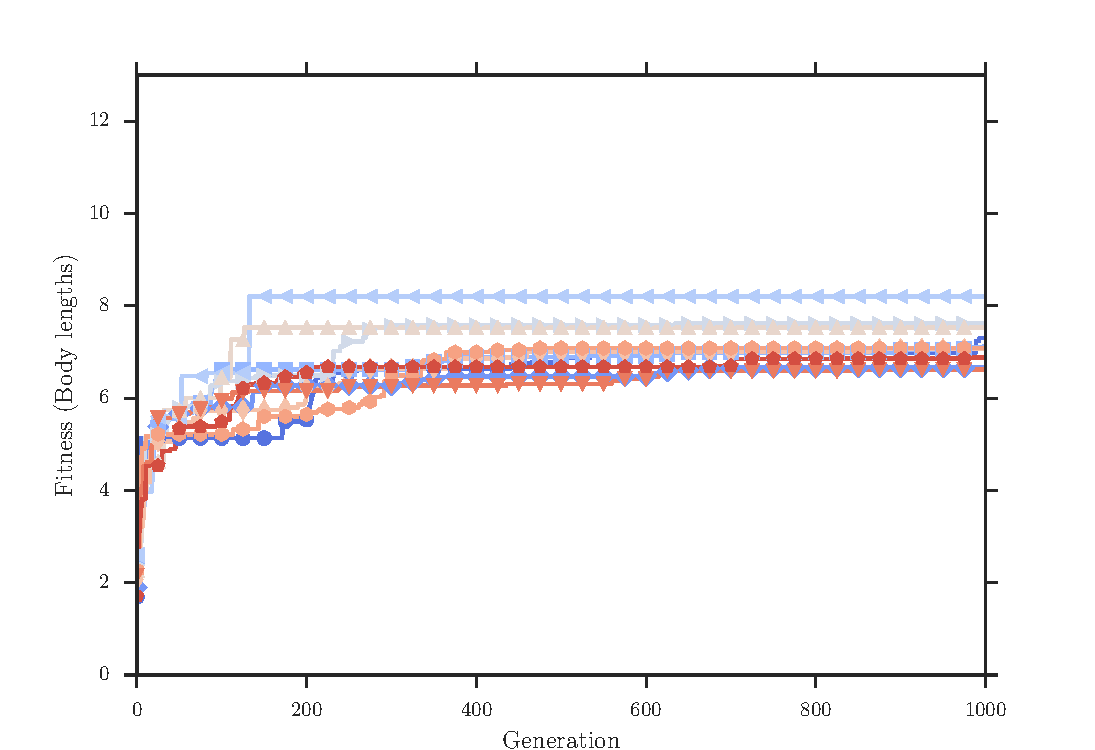
\includegraphics[width=1.0\textwidth]{../Figures/Results/indRunnAvgSize7Fitness.pdf}
\caption{Best so far fitness, $10$ individual runs for fitness based search. (Settings~\ref{Settings-size7})}
\label{fig:indRunsAvgSize10Fitness}
\end{figure}
~
\begin{figure}[ht!]
\centering
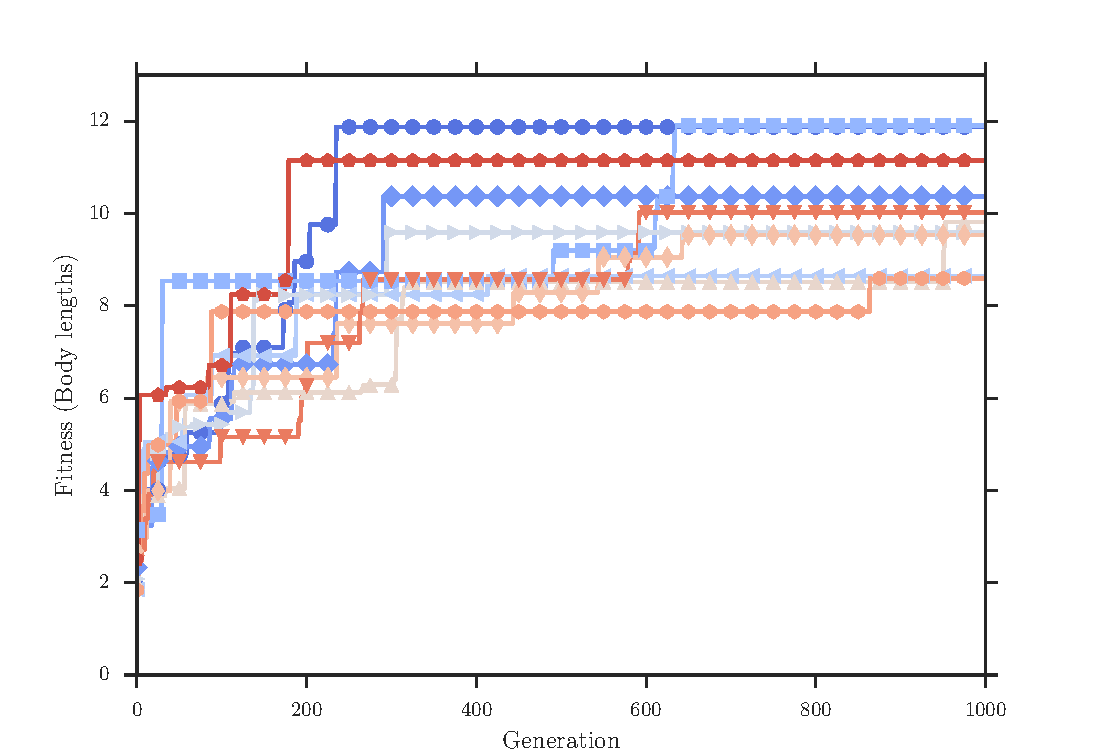
\includegraphics[width=1.0\textwidth]{../Figures/Results/indRunnAvgSize7Novelty.pdf}
\caption{Best so far fitness, $10$ individual runs for novelty search. (Settings~\ref{Settings-size7})}
\label{fig:indRunnAvgSize10Novelty}
\end{figure}

\section{Into The Performance of Novelty Search}

Before comparing novelty search to fitness based search, it is of interest to show how they individually behave under the same simulation settings.

Figure~\ref{fig:indRunsAvgSize10Fitness} shows $10$ independent runs for fitness based search. Following the gradient of the objective function, fitness based evolution does small steps towards better and more optimized solutions from generation to generation. However, fitness based evolution often sticks into specific morphologies which then tries to optimize leading the evolution to stop at these local maxima.

Figure~\ref{fig:indRunnAvgSize10Novelty} shows $10$ independent runs for the novelty search under the same settings. When compared to the fitness based search (see Fig.~\ref{fig:indRunsAvgSize10Fitness}) a clear difference can be observed. Evolving for novelty means that within the evolution only a novel behavior is rewarded instead of a good behavior or a behavior that leads to the optimization of the objective function. Fit individuals in respect to the objective function for which novelty search has no information within the evolution process, are results of new novel behaviors that novelty search seeks for. Observing only big steps in the fitness, we can derive that there is no optimization of specific morphologies within novelty search. Initially, novel individuals are highly rewarded, these individuals can be very good in respect to the fitness or not. On the next generations, mutations, crossovers, and copies of these novel individuals are not going to be highly variant in respect to their chromosome from their ancestors, resulting to similar behaviors. These not variant behaviors are not going to be remarkably rewarded in respect to their novelty value. Thus, highly novel individuals are producing less novel children in regards to their behavior. These children soft-robots, even though their fitness can be higher than their ancestors', having the potential to be optimized further, will not have the chance to reproduce in the next generations and be improved. 

\begin{figure}[t!]
\centering
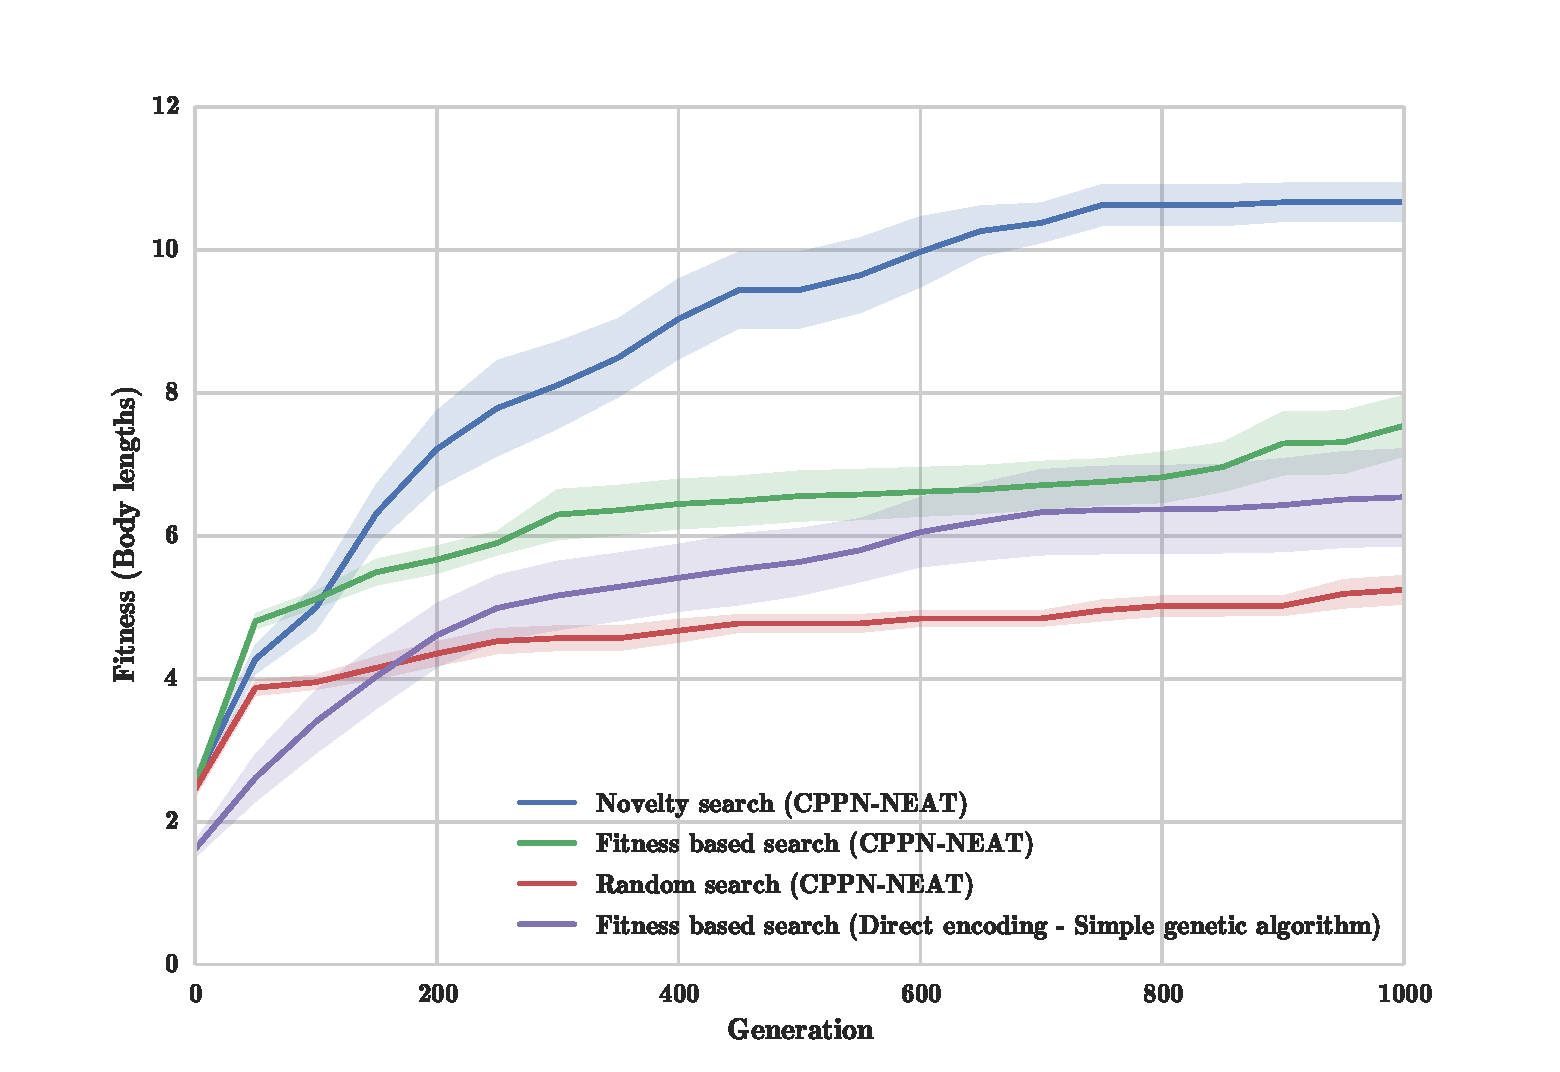
\includegraphics[width=1.0\textwidth]{../Figures/Results/FitNovRandomDirectSize5.pdf}
\caption{Comparison of simple genetic algorithm (direct encoding) against \emph{random} - \emph{fitness} - \emph{novelty} search with generative encoding. Best so far fitness averaged over $10$ runs. (Settings~\ref{Settings-size5})}
\label{fig:FitNovRandomDirectSize5}
\end{figure}

\begin{figure}[t!]
\centering
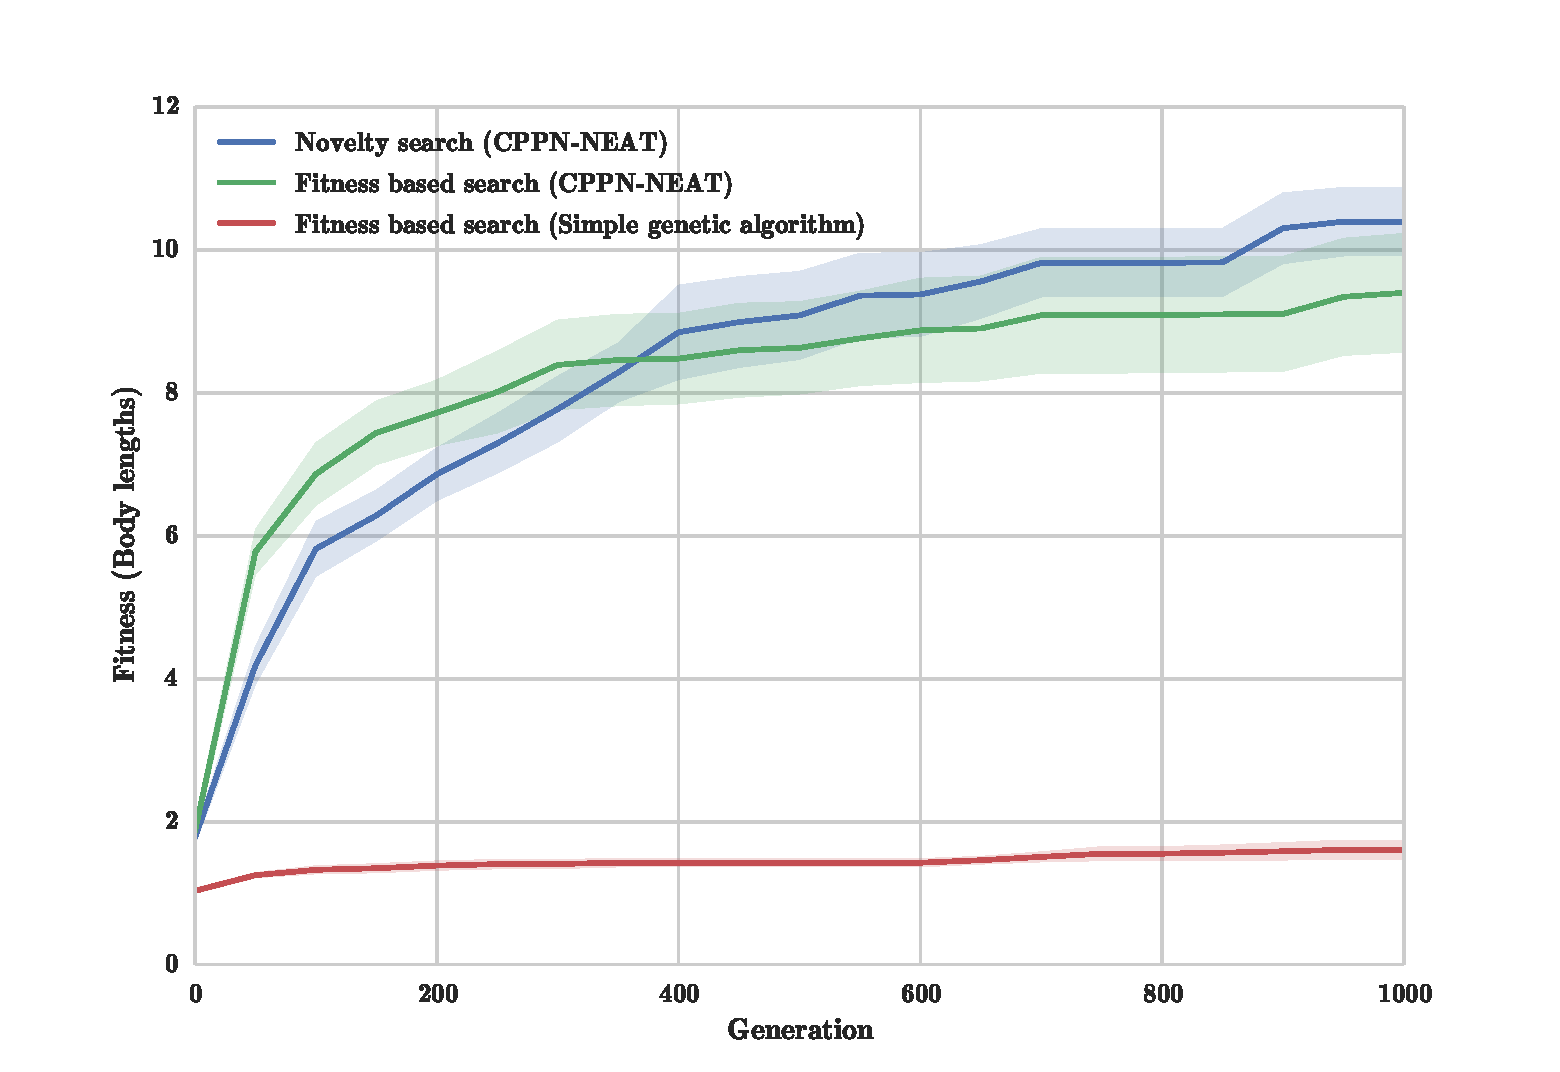
\includegraphics[width=1.0\textwidth]{../Figures/Results/FitvsNovVsDirSize10.pdf}
\caption{Comparison of simple genetic algorithm (direct encoding) against \emph{fitness} - \emph{novelty} search with generative encoding. Best so far fitness averaged over $10$ runs. (Settings~\ref{Settings-size10})}
\label{fig:FitvsNovVsDirSize10}
\end{figure}

To extensively compare the performance achieved by novelty search method in the same experiment held under two different simulation settings (for sizes $5^3$ ,$10^3$), set side by side with fitness search, random search, and finally a simple genetic algorithm. Notice, that the first three methods are referring to a generative encoding (CPPNs) evolved by CPPN-NEAT evolutionary algorithm and using selection in respect to fitness, novelty and finally random selection, while the last uses a direct encoded genome driven by fitness. 

Two dimensional trajectories as described in the previous chapter (see Sec.~\ref{BehaviorNoveltySearch}), are used by novelty search in order to describe the novelty in the behavior space. The objective function that describes the goodness of solutions is the displacement of the soft-robot's center of mass from its initial position in body-lengths, and it is used for all fitness-based search methods. Random selection in CPPN-NEAT achieved choosing random selected individuals to breed on each generation. For direct encoding, direct encoded genomes represent the solutions as described in Section~\ref{DirectEncodingEvolution}.

Figure~\ref{fig:FitNovRandomDirectSize5}, presents the results for the low resolution soft-robots ($5^3$). The average best so far displacement of the soft-robots in body lengths is presented alongside the deviation error. Notice, the difference between novelty search and the other methods. Novelty evolves structures that are superior than any other method does in these settings. It should be mentioned that in such a small structures complex locomotion patterns cannot be evolved due to the stability issues of the simulator, and because of the fact that lightweight structures can be bouncy, leading to ball shaped structures capable of achieving large displacement from their initial positions. That being said, we still have to deal with an optimization problem, where local optima and global ones can be found as the number of the possible solutions in this setting, using 4 materials, is $\sim 2,3 \times 10^{87}$. Using the two-dimensional trajectories of the soft-robots, novelty search visits optimal solutions that none of the other methods does. Local optima can prevent fitness-based search to achieve the performance of novelty search. Encoding limitations in direct encoding cannot lead to optimal solutions for this settings. In the case of random search, the individuals of each generation are selected randomly to reproduce. Having neither the information about their fitness, nor the driving force of novelty search that seeks for novel behaviors, it fails to evolve any decent locomotion. The only reason random search in CPPN-NEAT achieves to develop displacement of $\sim 5$ body-lengths, is the powerful encoding used (CPPNs). The simple genetic algorithm approach which uses a direct encoded chromosome to represent the structure of the soft-robots performs better than using random selection with an indirect encoding. Structural symmetry and regularity does not provide all of its merits in such a low resolution settings.

Moving to a higher resolution for the lattice, it is expected that generative encoding will prove its advantages over the direct encoding scheme~\citep{cheney2013unshackling,stanley2007compositional}. 
\begin{figure}[t!]
\centering
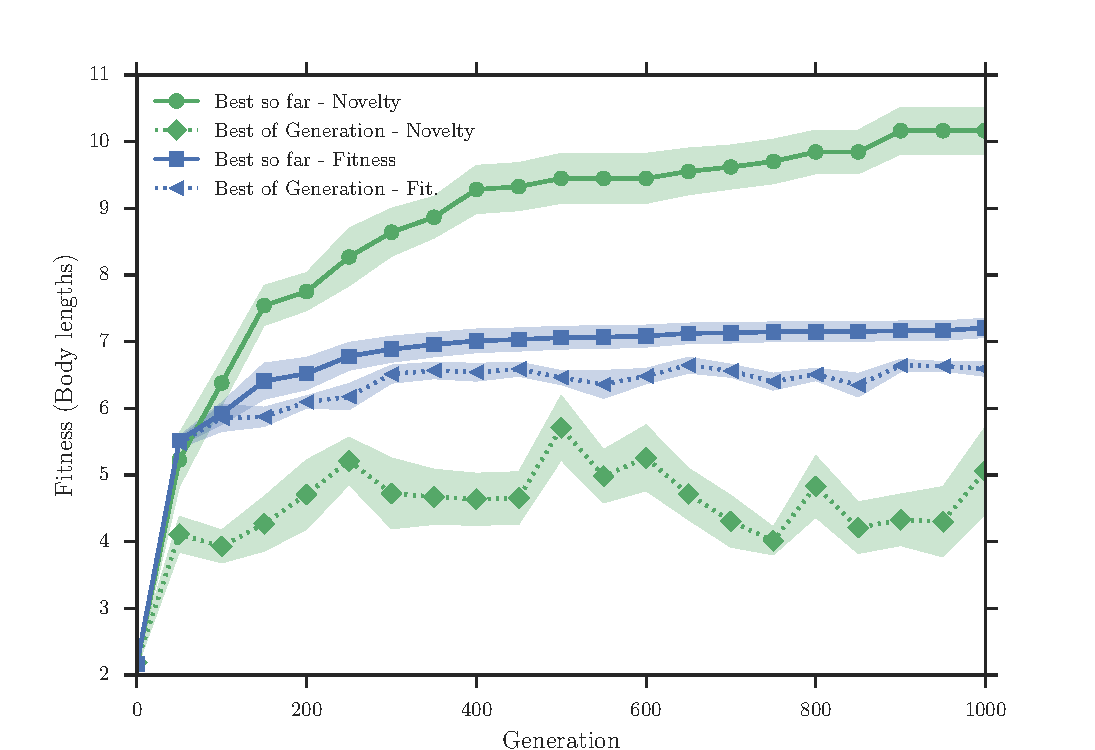
\includegraphics[width=1.0\textwidth]{../Figures/Results/AvgGenerChampNoveltyFitnessSize7.pdf}
\caption{Fitness of the generation's champion (best individual) for \emph{fitness} - \emph{novelty} search averaged over $10$ runs. (Settings~\ref{Settings-size7})}
\label{fig:AvgGenerChampNoveltyFitnessSize7}
\end{figure}
Furthermore, novelty search now has a more difficult task as the space of possible behaviors, two-dimensional trajectories, becomes larger as more complicated morphologies can now be produced (morphology space for $10^3$ lattice space: $9.3 \times 10^{698}$). These morphologies can achieve life-like locomotion. The same experiment as before held under a lattice resolution of $10^3$. Figure~\ref{fig:FitvsNovVsDirSize10}, presents the results of the four different methods in these higher resolution settings. Results reassure that novelty search achieves higher fitness on average against fitness-based search. Nevertheless, there is no tremendous difference as in the previous experiment. Both methods achieve to evolve the soft-robot structure with the highest fitness found in all experiments ($\sim 14$ Body lengths). Novelty search behaves more constant in evolving individuals with high fitness in all runs, on the other hand most of individual runs of fitness search are being trapped in a low fitness local optima, trying to optimize specific individuals without trying to explore deeply the fitness landscape like novelty search does successfully. Random selection within CPPN-NEAT evolution produced low-fitness morphologies for soft-robots. The high difference between random selection evolution and novelty search proves that the behavior of novelty search cannot be considered as a random search. Backtracking (visiting same behaviors) of random search methods is a crucial variable for the evolution. The superiority of generative encoding (CPPN) over direct encoding can evidently be observed. Regular in shape morphologies can take advantage of their geometrical properties to locomote efficiently. CPPNs (see Section~\ref{CPPN}) are proven to be successful in creating these morphologies. The performance of direct encoding when a higher resolution lattice is used for the soft-robots, was radically decreased. The structure and morphology regularity is a necessity for soft-robots in order to perform decently in this resolution settings, a property that direct encoding cannot capture failing in this resolution.

\begin{figure}[t!]
\centering
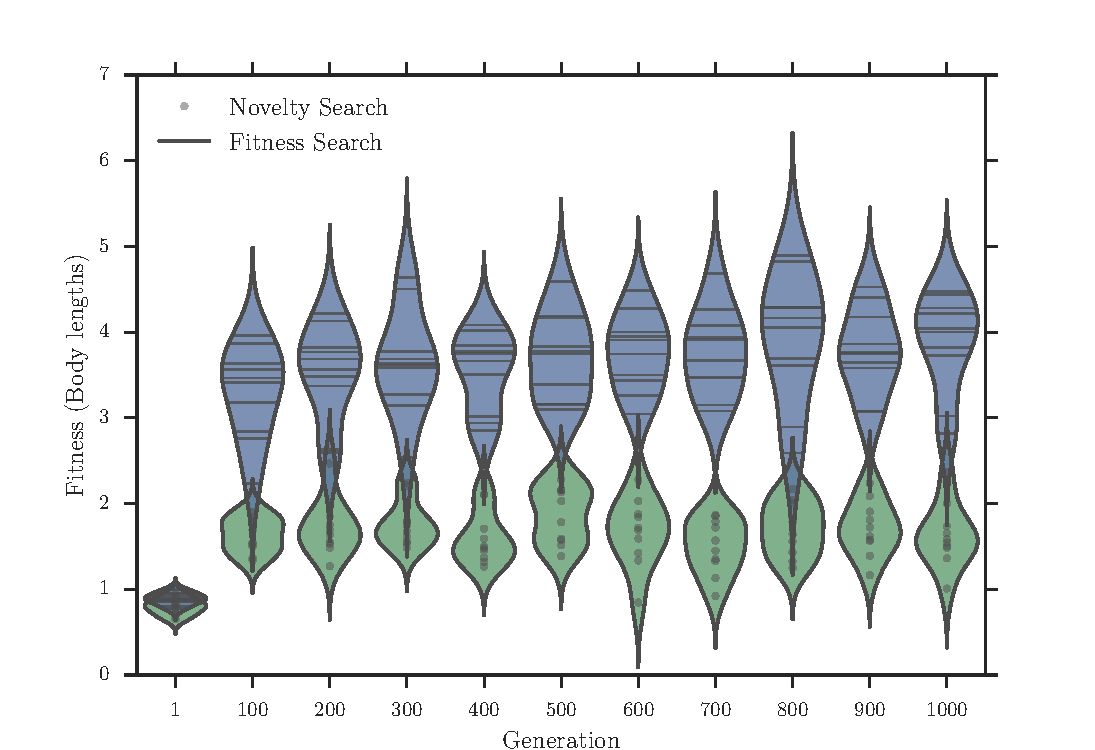
\includegraphics[width=1.0\textwidth]{../Figures/Results/ViolinPlotsAvgGenFitSize7.pdf}
\caption{Distributions of average population fitness per generation over 10 runs for \emph{fitness}(Blue) - \emph{novelty} (Green) search with generative encoding. (Settings~\ref{Settings-size7})}
\label{fig:ViolinPlotsAvgGenFitSize7}
\end{figure}

Novelty search achieved to improve the average displacement of the soft-robot morphologies. The metric that both search methods are compared against each other, is the best so far fitness. Only the champions of each generation can affect this metric. An important question at this moment, is how the population of each generation is affected regarding the search method that is followed. The average fitness of the population, as well as the champion's fitness are two cues that can give interesting properties of each search. Figure~\ref{fig:AvgGenerChampNoveltyFitnessSize7}, presents the fitness of the champion soft-robot (best within the generation), alongside the best so far fitness for both novelty and fitness-based search, averaged over $10$ evolution runs. In fitness-based search there is a trend that champions of each generation are getting better through the evolution, resulting to an approximately monotonically increasing function. 
\begin{figure}[t!]
\centering
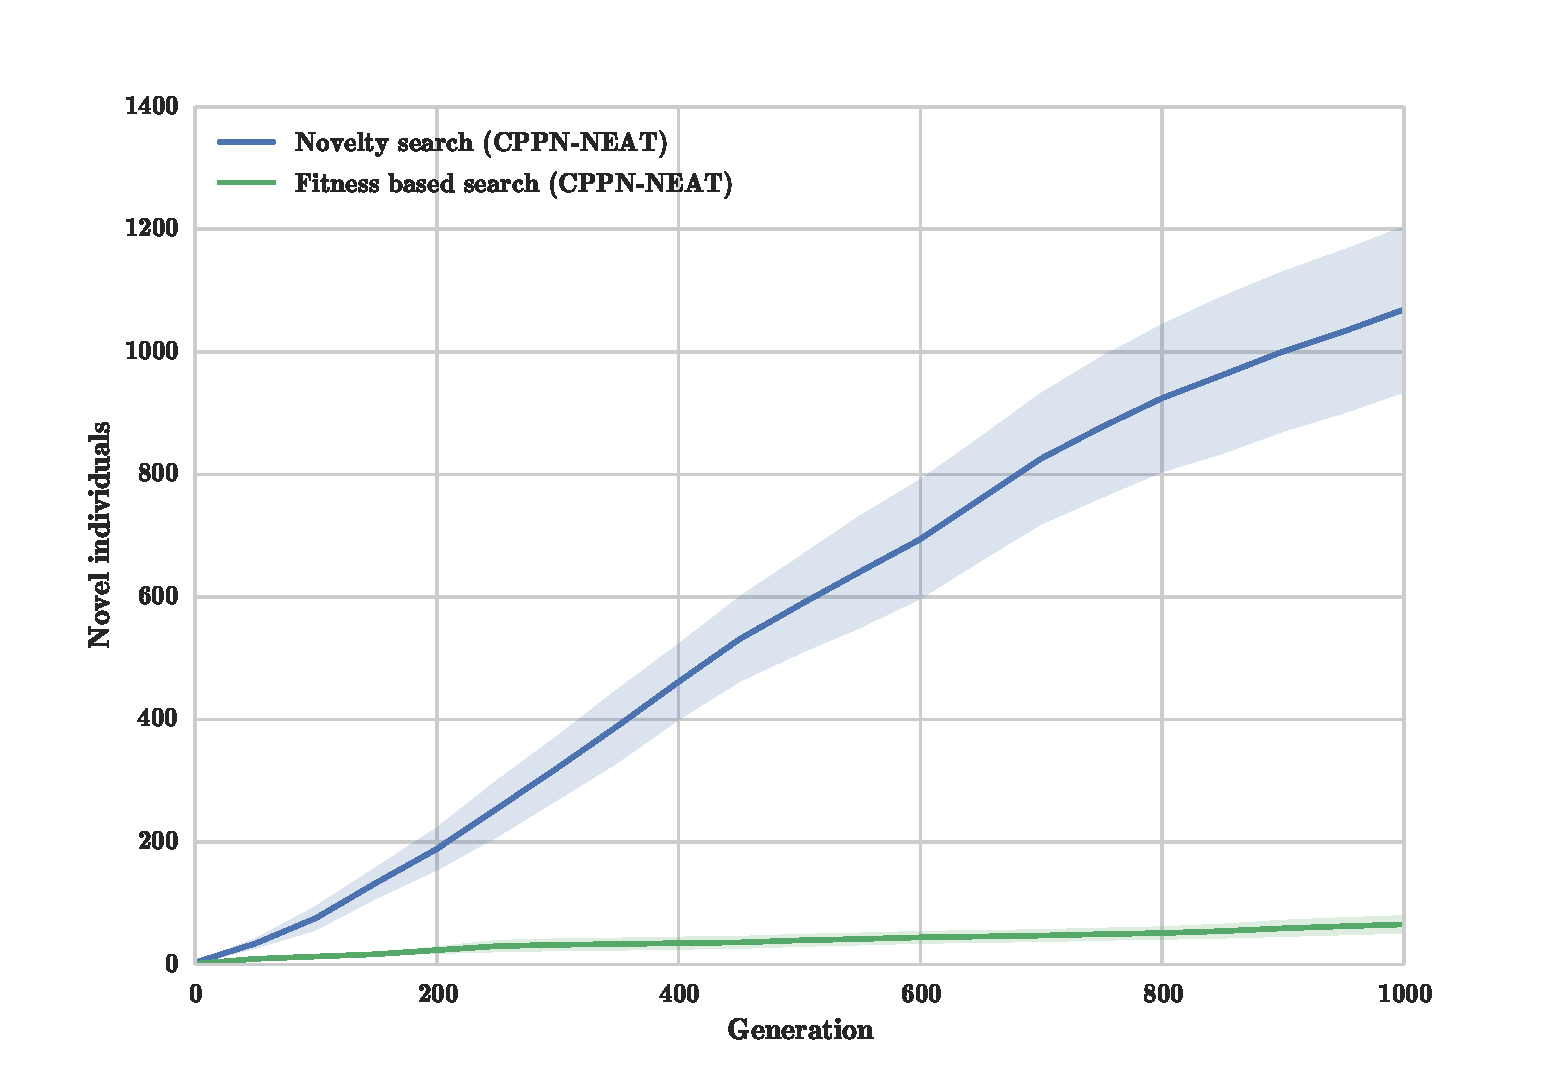
\includegraphics[width=1.0\textwidth]{../Figures/Results/novelIndividualsFitNovComp.pdf}
\caption{Number of novel behaviors found up to generation number, averaged over 10 runs. The novelty measure is computed as the average distance from the $10$-nearest behaviors for \emph{fitness} - \emph{novelty} search with generative encoding. (Settings~\ref{Settings-size7})}
\label{fig:novelIndividualsFitNovComp}
\end{figure}
However, a random pattern can be observed in generation champions of novelty search. An early improvement is mainly caused by the generative encoding, while the performance of the generations' champions is not affected by the search towards novel behaviors. What is interesting here to see is that on average the champions during novelty search evolution are worse than those fitness search evolves, whereas the best so far fitness is better for novelty search in this setting (lattice resolution $7^3$). Hence, individuals that resulting in the increased performance of novelty search clearly lie on the tail of the fitness distribution on each generation. In the same fashion, the average fitness of each generation seems also affected by the different optimization method. Figure~\ref{fig:ViolinPlotsAvgGenFitSize7} illustrates the distribution of the average fitness per generation over $10$ independent runs for novelty and fitness based search. The average fitness of each generation is been shown for every $100$ generations. The violin-like distributions show that the average fitness per generation remains stable through the whole evolution ($1000$ generations) for both methods. Additionally, the generations' average fitness is significantly lower for novelty search, meaning that when the evolution is being carried towards novel behaviors there is no such guarantee that novel findings in the behavior space are also  fit solutions. What has been shown in the last two figures (see Figs.~\ref{fig:AvgGenerChampNoveltyFitnessSize7},\ref{fig:ViolinPlotsAvgGenFitSize7}), evidently shows that even though novelty search achieves in finding more ``fit'' solutions than fitness based search in the specific problem domain, the average fitness of both generation champions and population remain lower than in fitness based search.


Until this point, the performance of both fitness and novelty search methods have been compared in the same objective metric, the displacement of the produced soft-robot morphologies. The former method tries to optimize genomes in respect to the specific objective function, while the latter is focusing the search into creating diversity of the population in the behavior level. It is of interest to show the performance of both methods in a different evaluation metric. The evaluation metric is used in this experiment is the number of novel behaviors generated within an evolution run. Inverting the evaluation metric so that it is in favor of novelty search, it is expected that novelty search will outperform fitness-based search by a huge margin. Figure~\ref{fig:novelIndividualsFitNovComp}, presents the number of novel behaviors that the two evolutionary methods generated, averaged over $10$ runs. Both methods used the same settings (behavior/constant values) to determine a novel behavior. The resulted plot shows that comparing these two methods in this metric is pointless as novelty search drives the evolution towards spaces in the behavior space that have not been visited. Resulting in such a way to produce $\sim 1$ novel behavior per generation. Novelty search achieves better performance than fitness-based search in both objectives set so far, creating fit, and at the same time diverse solutions.
\begin{figure}[t!]
\centering
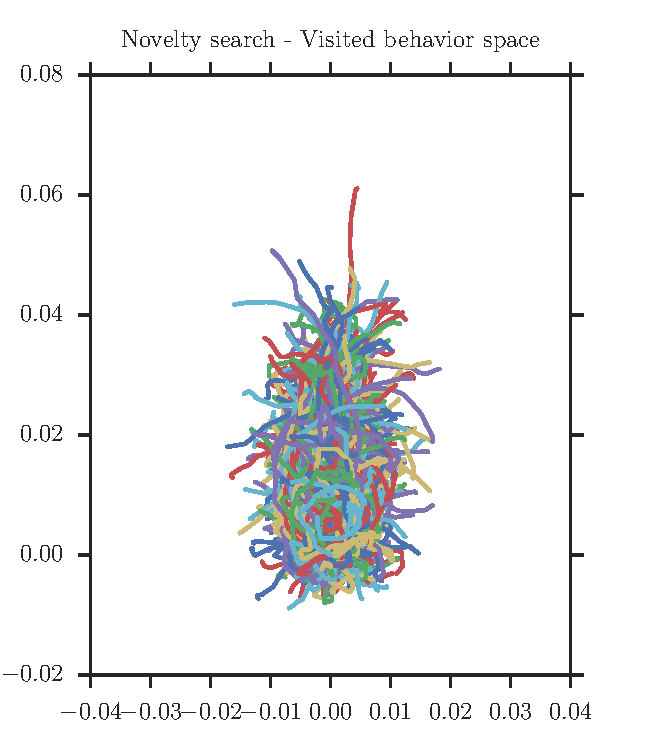
\includegraphics[width=0.49\textwidth]{../Figures/Behaviors/behaviorsNovelty.pdf}\	
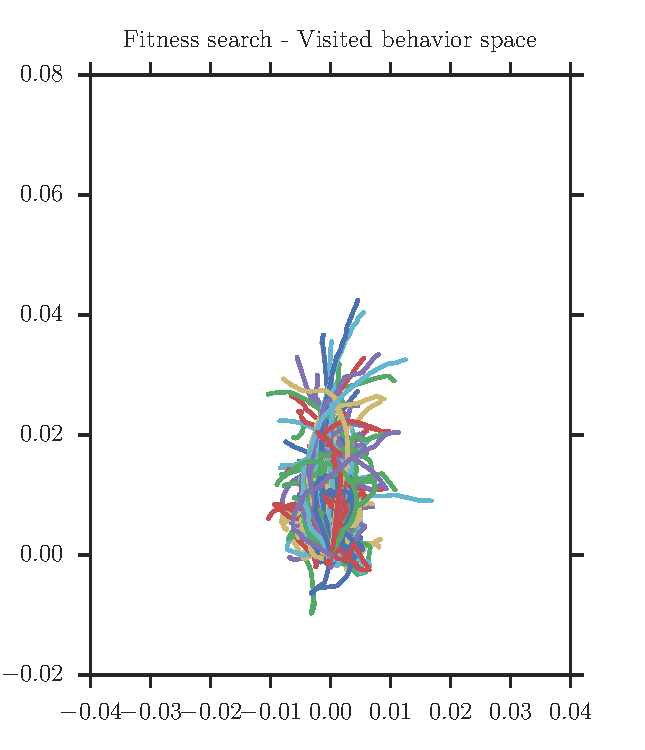
\includegraphics[width=0.49\textwidth]{../Figures/Behaviors/behaviorsFitness.pdf}
\caption{Novelty search creates a vast amount of behaviors achieving in this way to find fit individuals, and avoid local optima of the solution space. (Settings~\ref{Settings-size7})}
\label{fig:behaviorSpaceDiversity}
\end{figure}
To visualize the difference in the behavior space of the two methods, Figure~\ref{fig:behaviorSpaceDiversity}, illustrates all the stored found novel behaviors (two dimensional trajectories) found in one evolution run of novelty and fitness-based search. The initial position of the soft-robots is the start of the axes, and the centroid of the trajectories is normalized to be perpendicular to the horizontal axis. The differently colored trajectories verify that novelty search searches the space of behaviors more than fitness-based search does. In addition, observing the performance of these trajectories, is easy to interpret that longer trajectories (higher fitness) have been evolved by the first method. 

In this section, the performance and several aspects of novelty search has been discussed. Novelty-search achieved higher average displacement of the evolved soft-robots against traditional fitness-based search, when two dimensional trajectories used to define the behavior in all settings (lattice resolution of $5^3$, $7^3$, and $10^3$).


\begin{figure}[t!]
\centering
\begin{subfigure}[b]{1.0\textwidth}
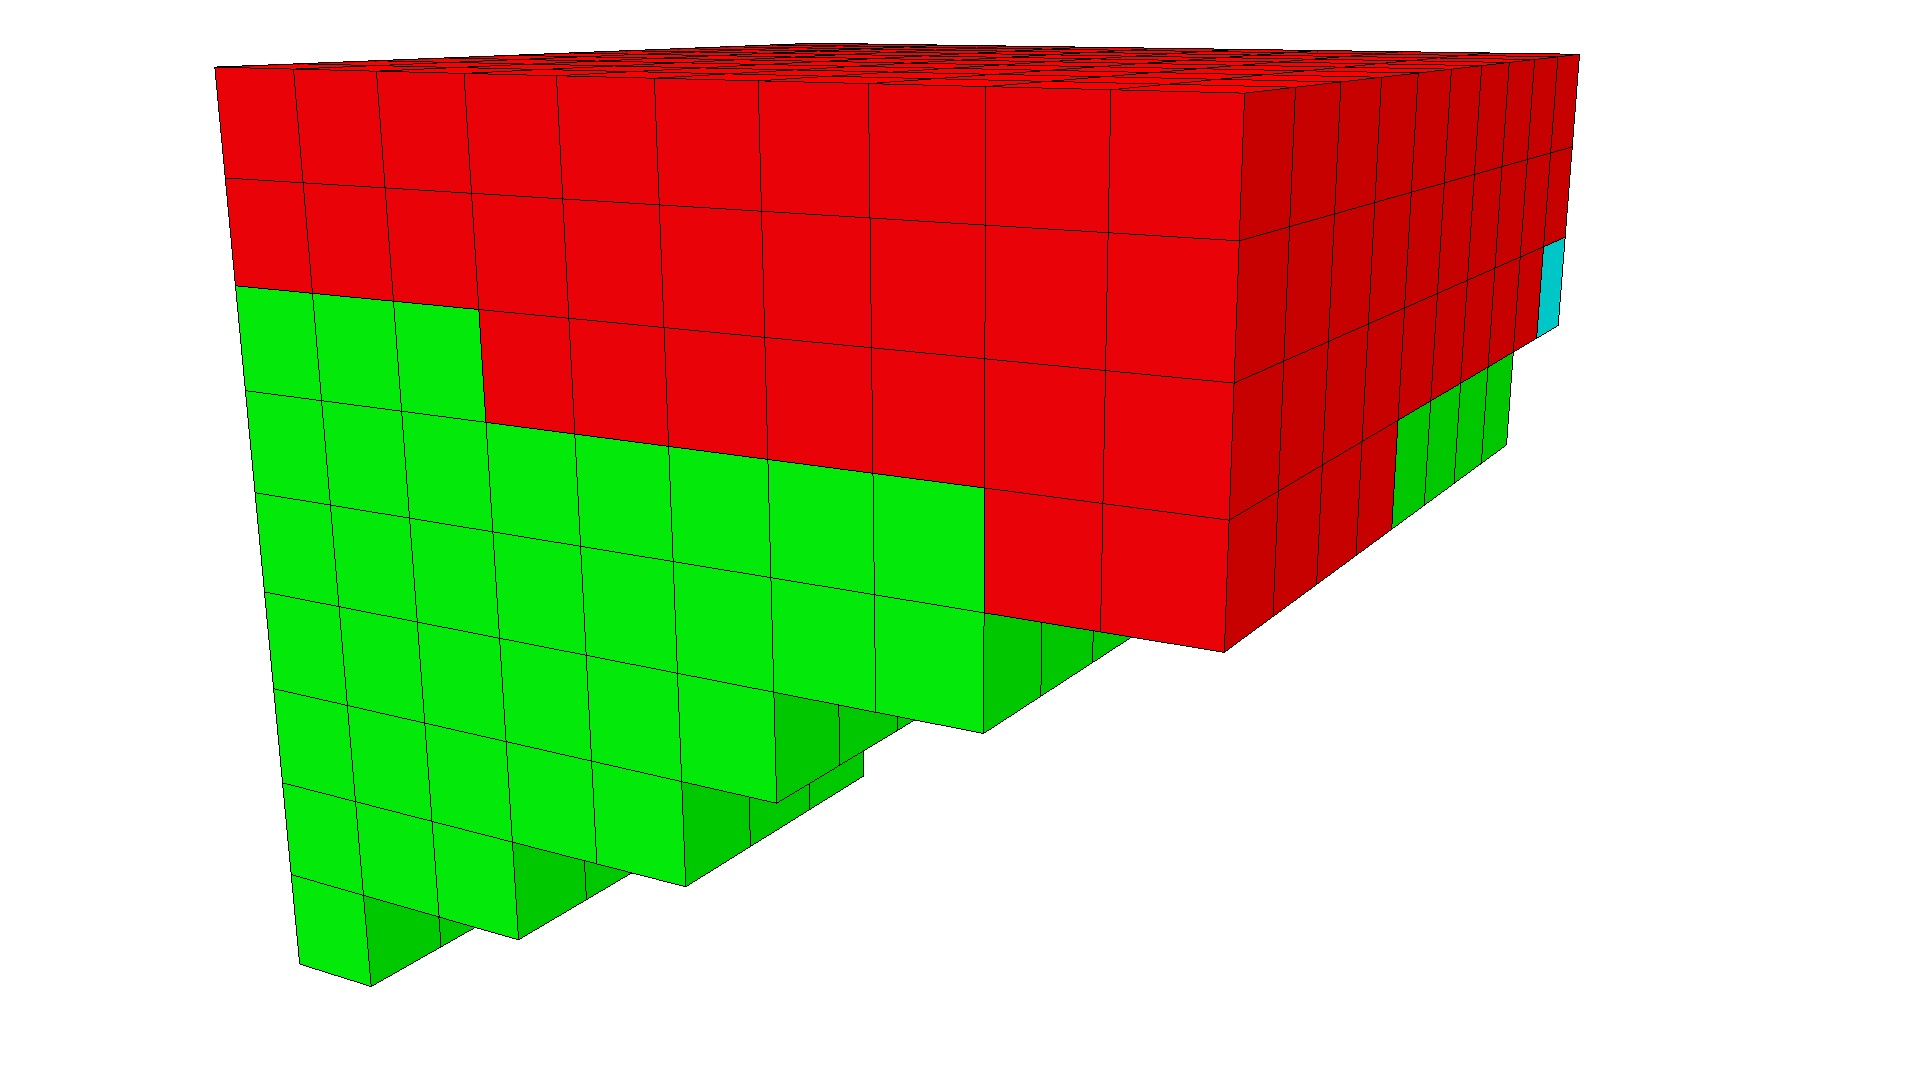
\includegraphics[width=0.19\textwidth]{../Figures/Robots/f_4_g_100.jpg}
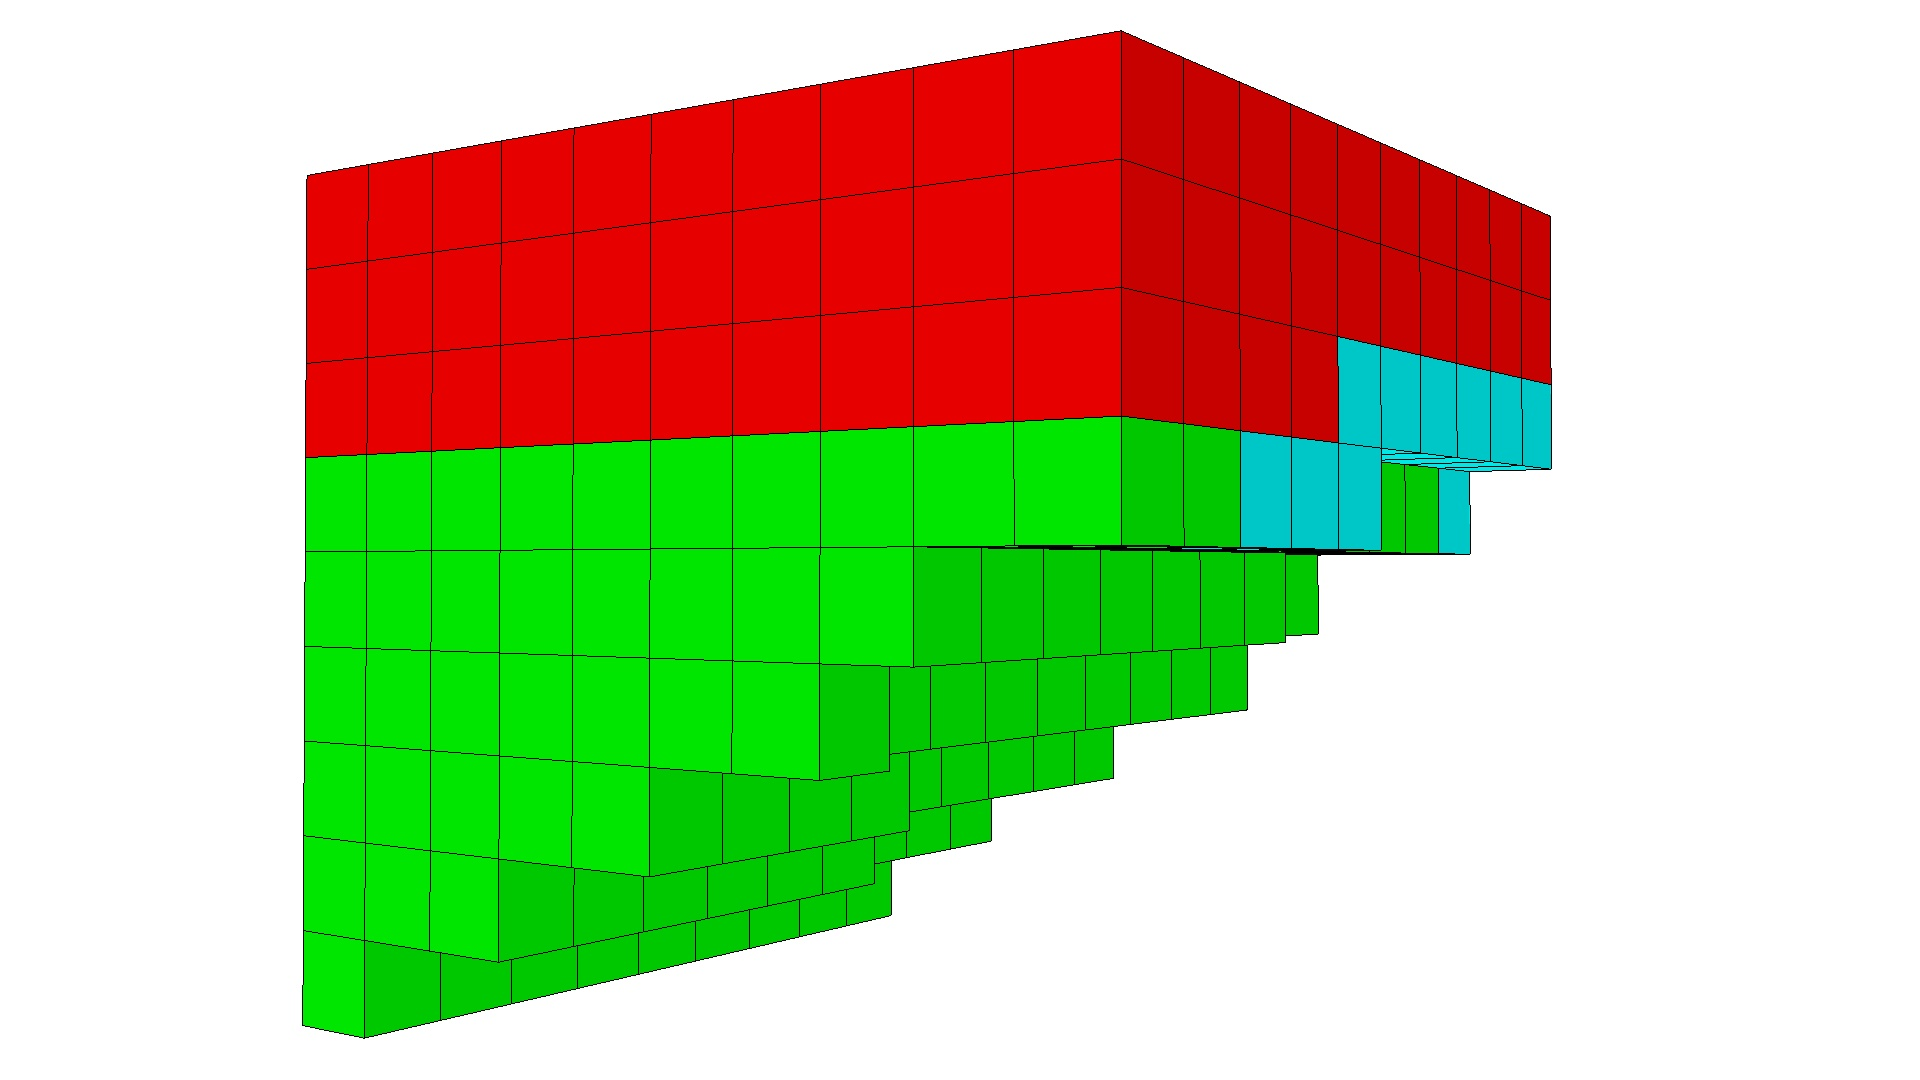
\includegraphics[width=0.19\textwidth]{../Figures/Robots/f_4_g_200.jpg}
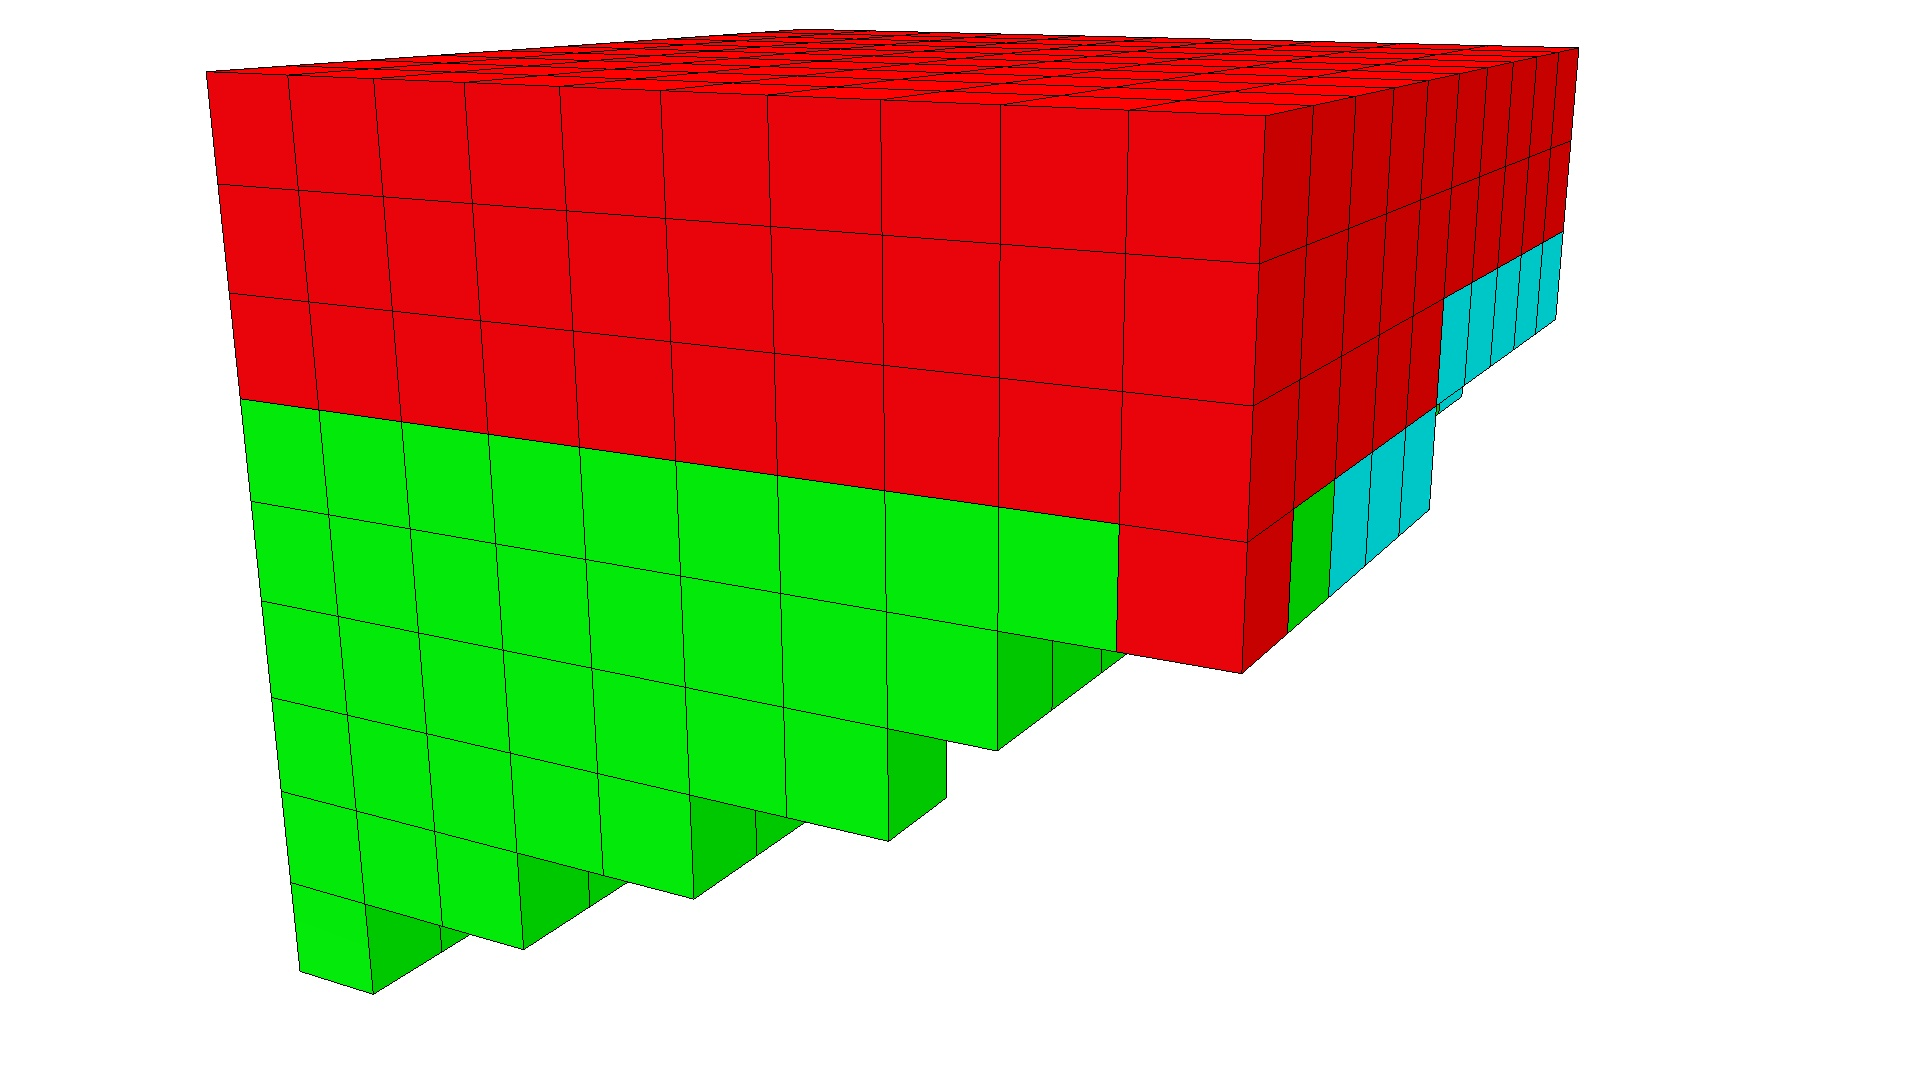
\includegraphics[width=0.19\textwidth]{../Figures/Robots/f_4_g_300.jpg}
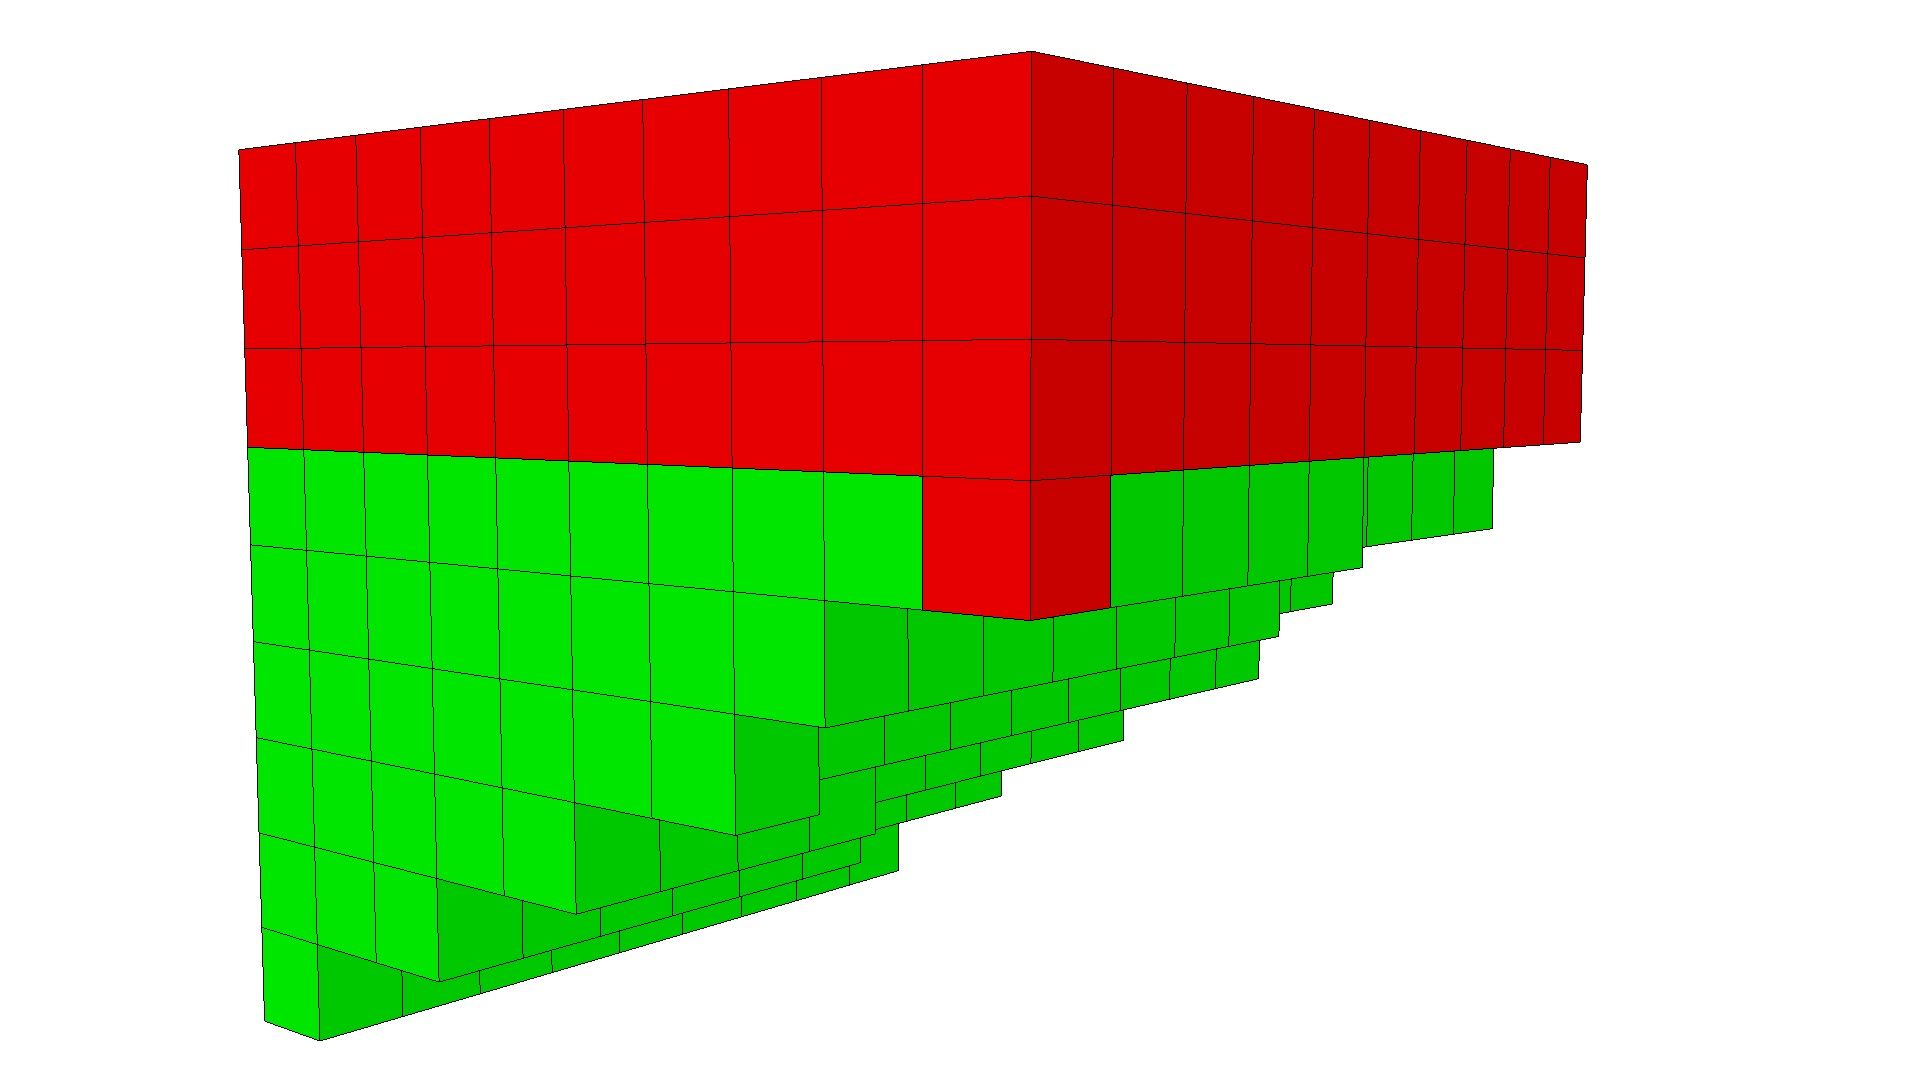
\includegraphics[width=0.19\textwidth]{../Figures/Robots/f_4_g_400.jpg}
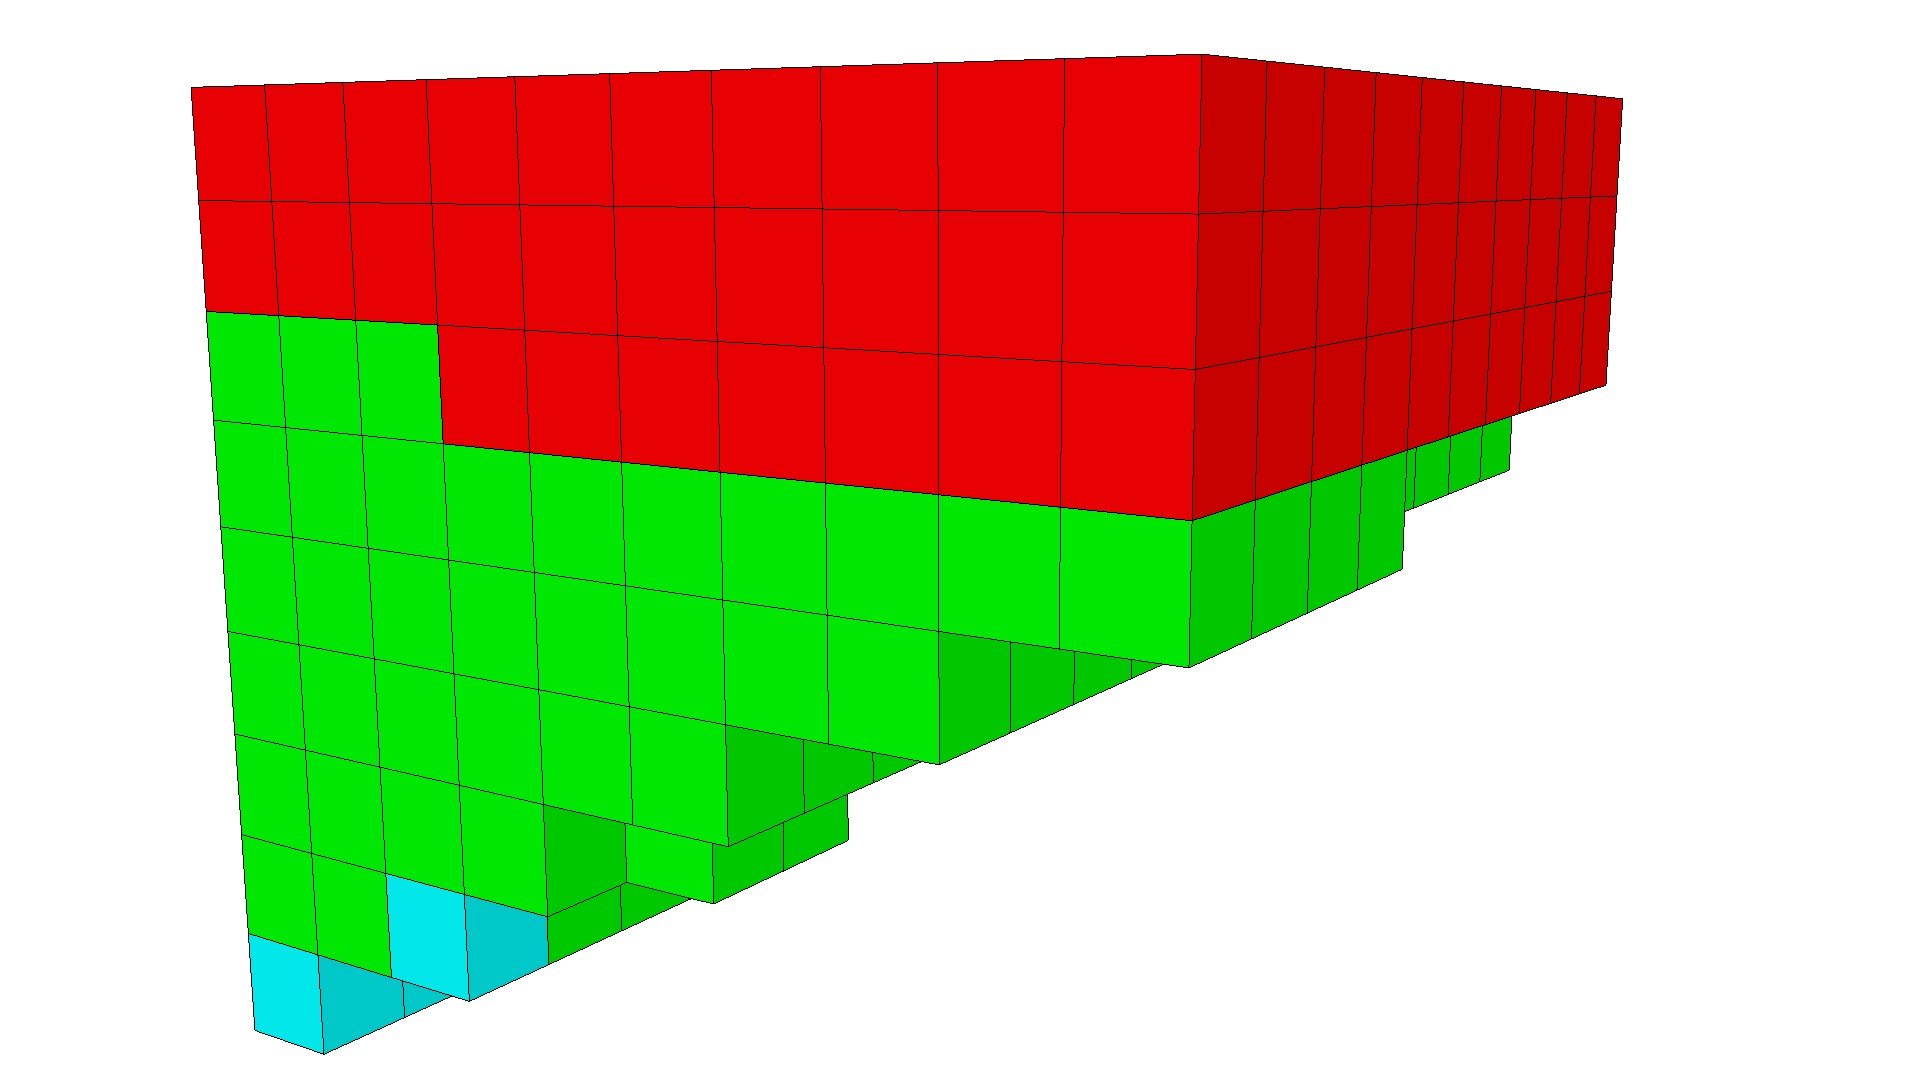
\includegraphics[width=0.19\textwidth]{../Figures/Robots/f_4_g_500.jpg}\\
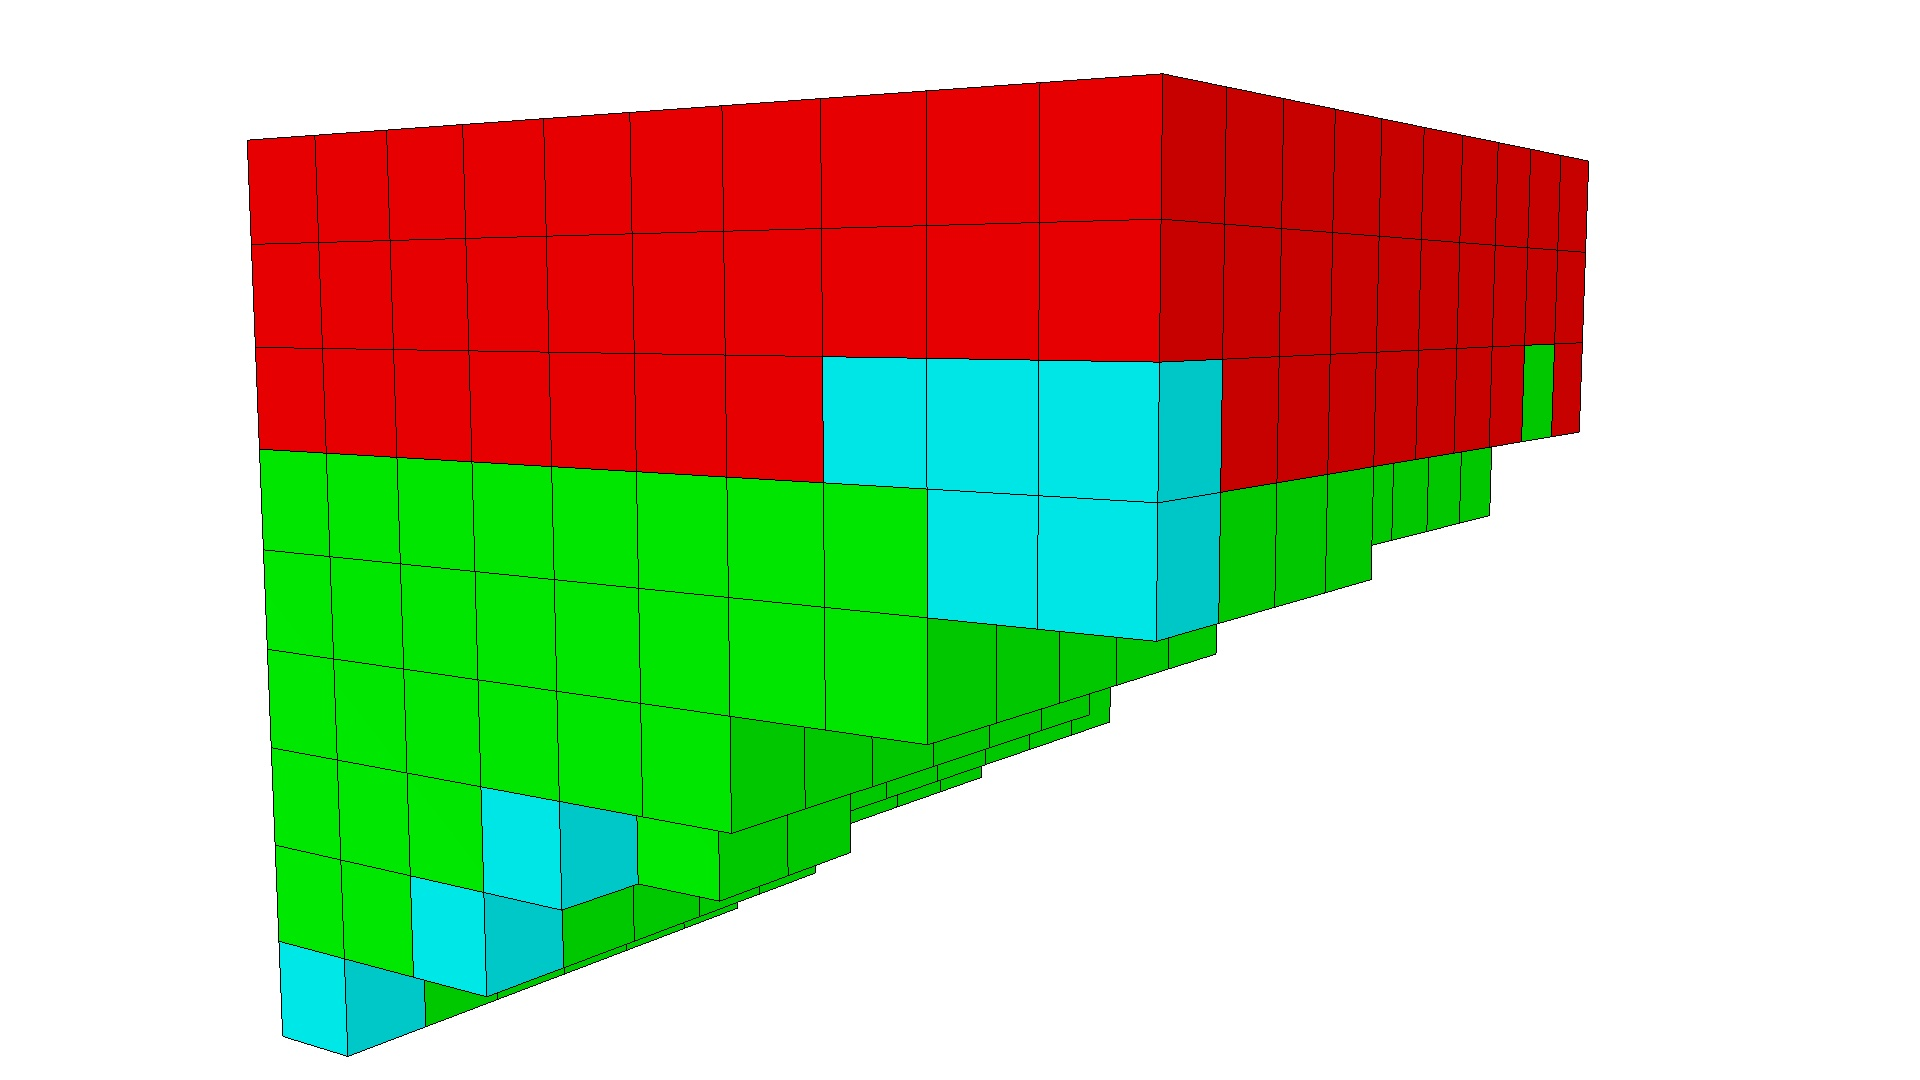
\includegraphics[width=0.19\textwidth]{../Figures/Robots/f_4_g_600.jpg}
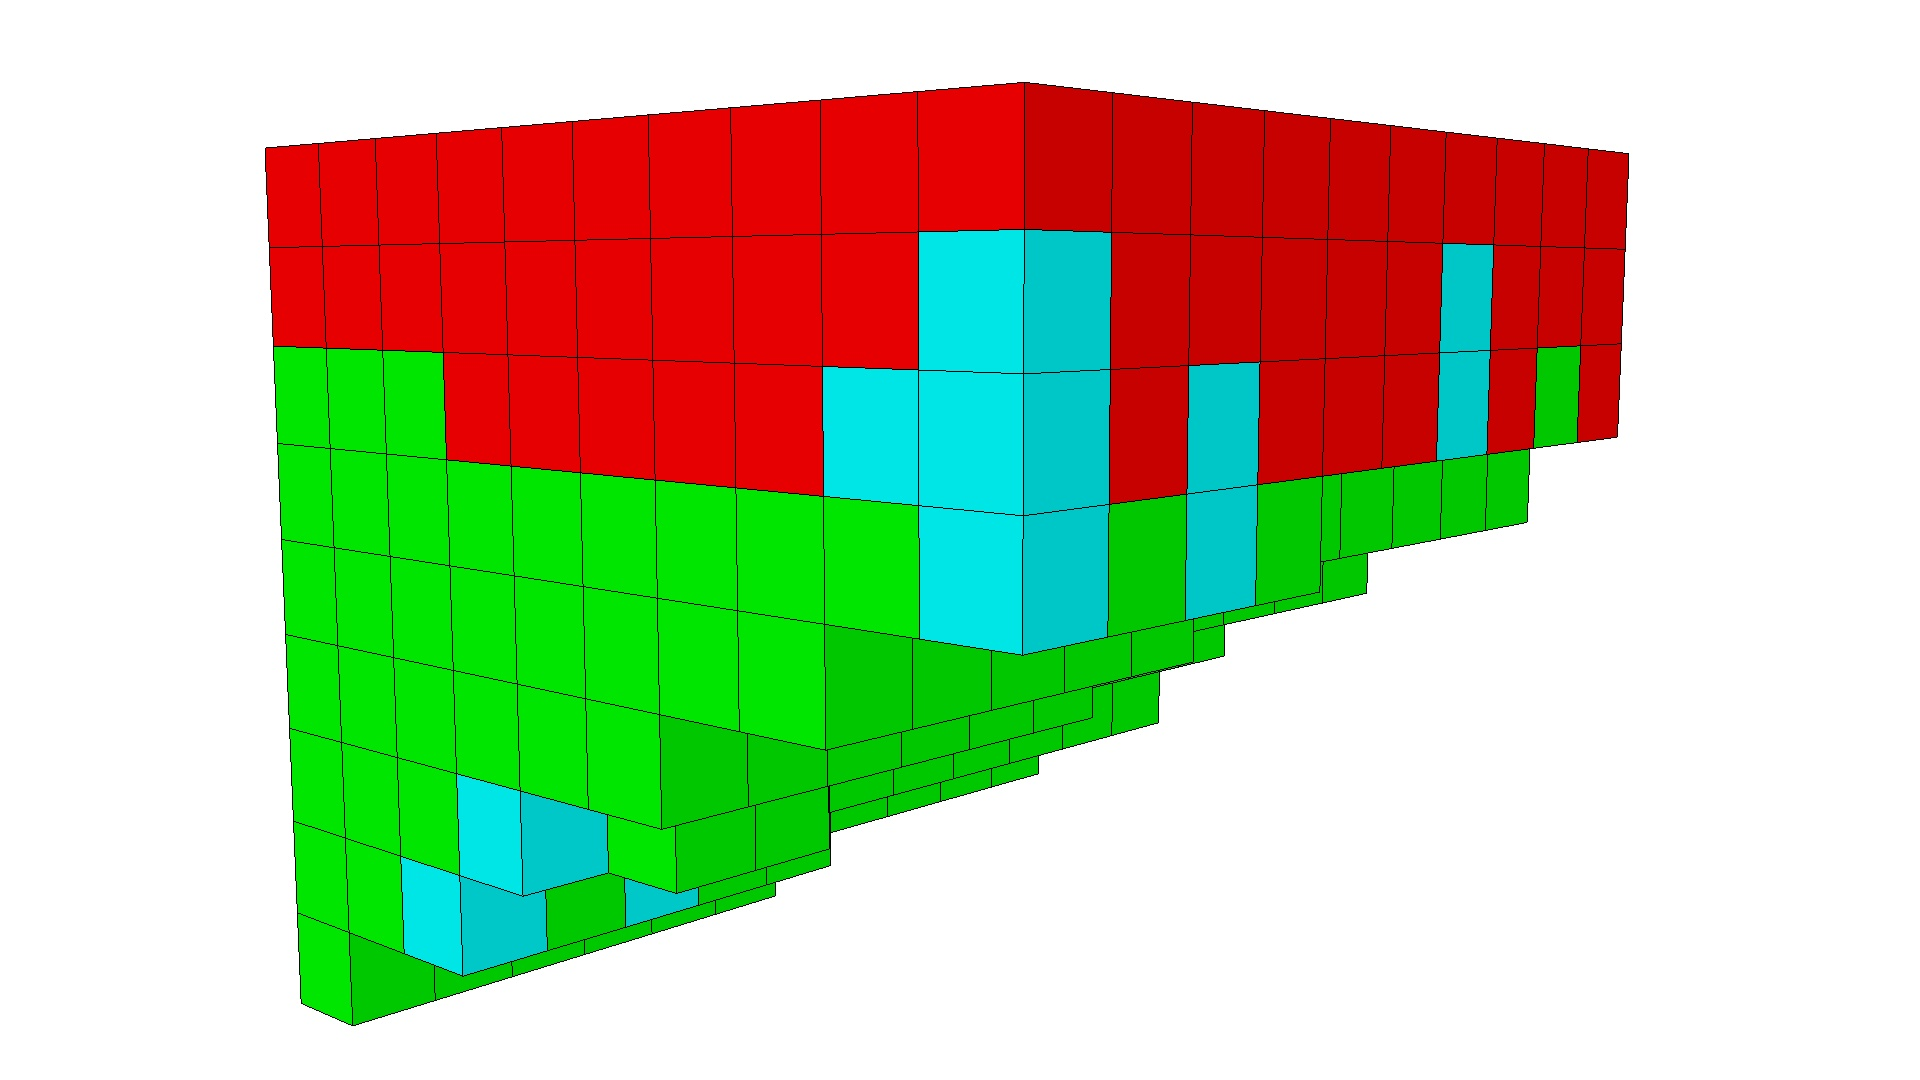
\includegraphics[width=0.19\textwidth]{../Figures/Robots/f_4_g_700.jpg}
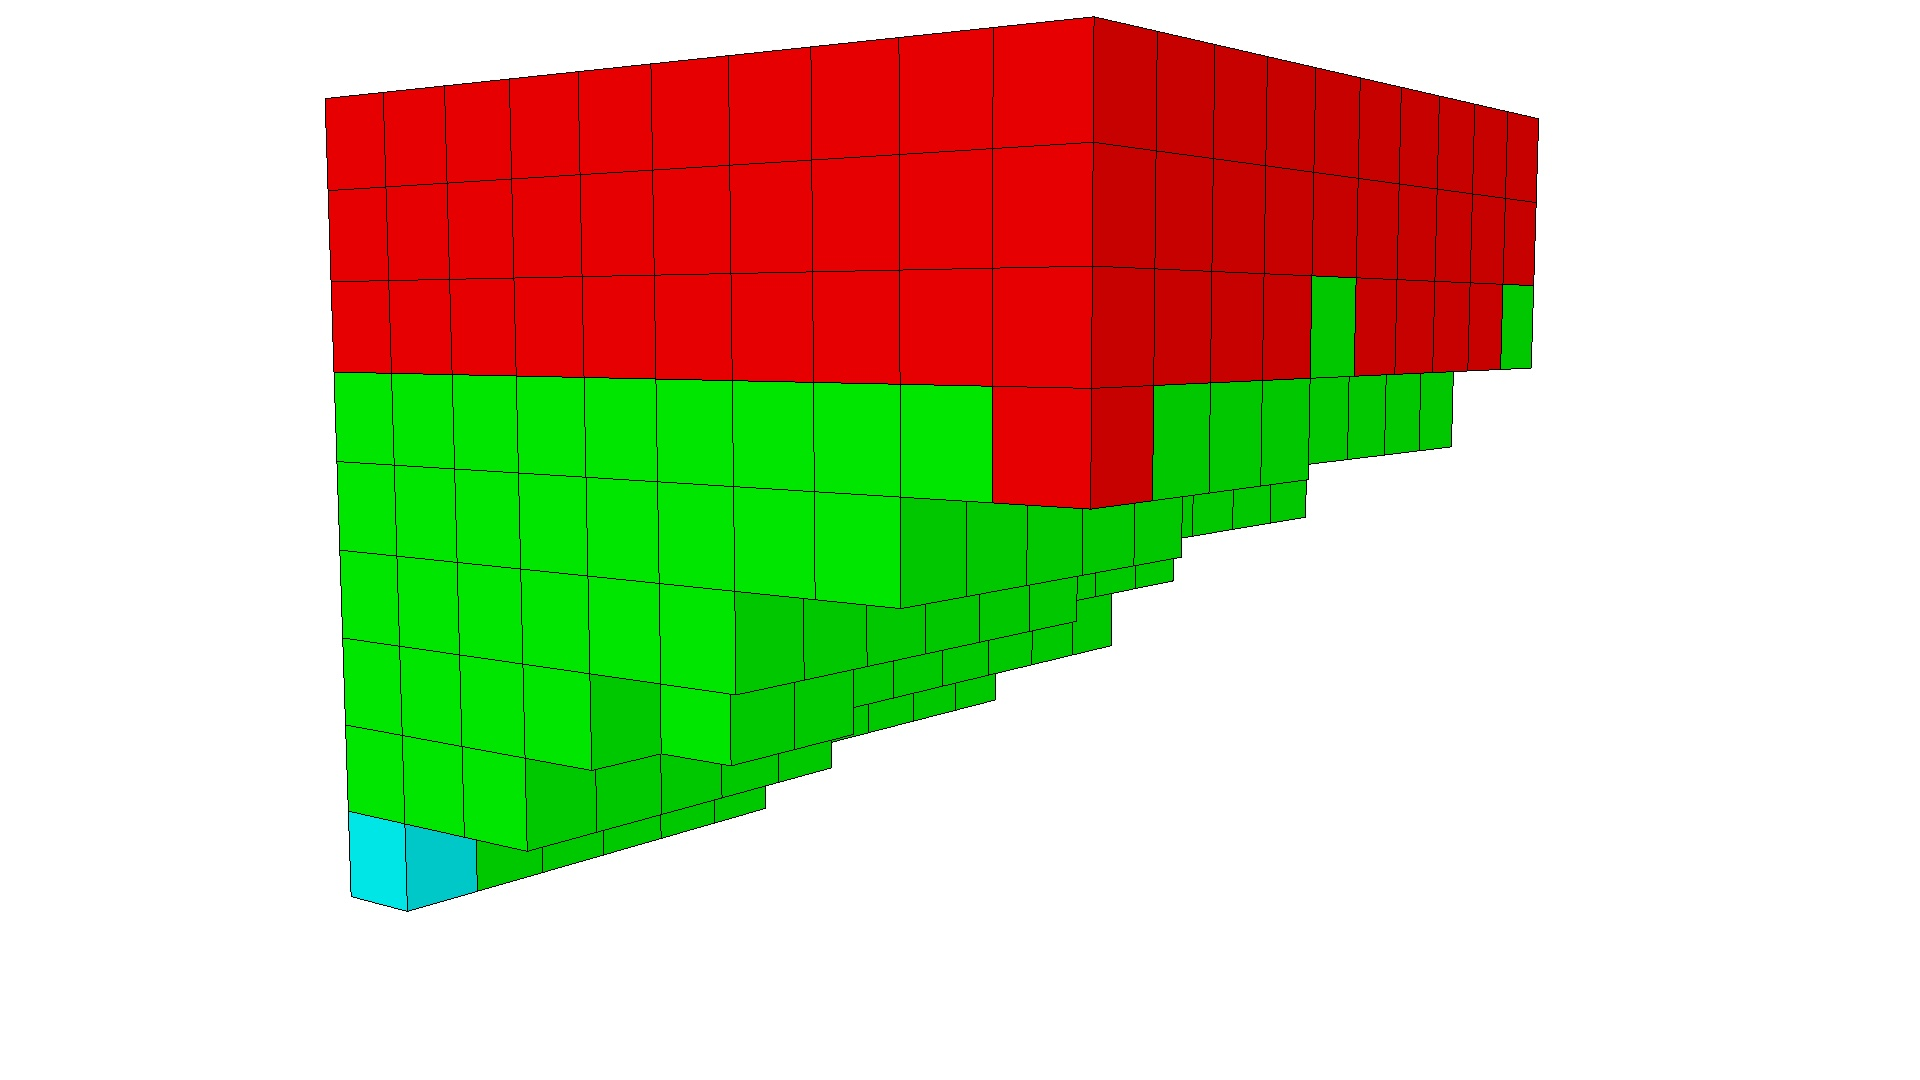
\includegraphics[width=0.19\textwidth]{../Figures/Robots/f_4_g_800.jpg}
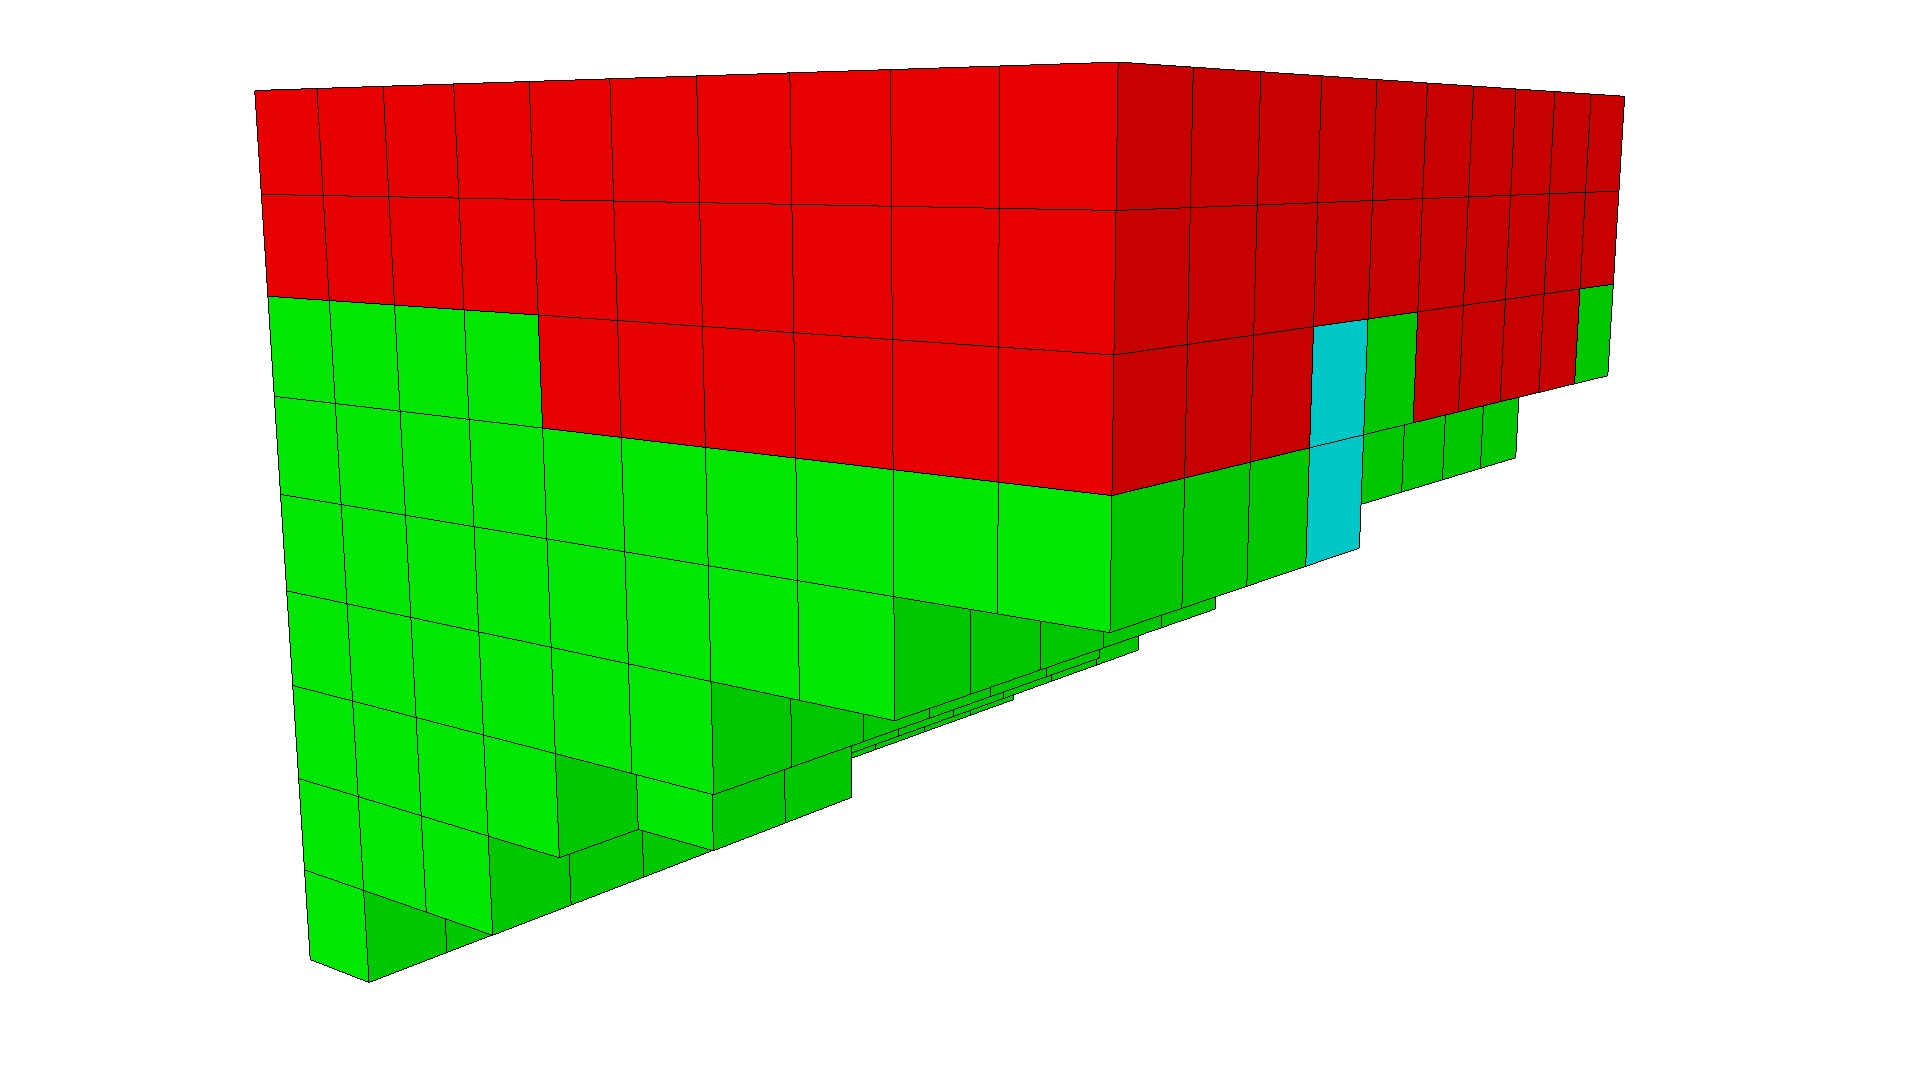
\includegraphics[width=0.19\textwidth]{../Figures/Robots/f_4_g_900.jpg}
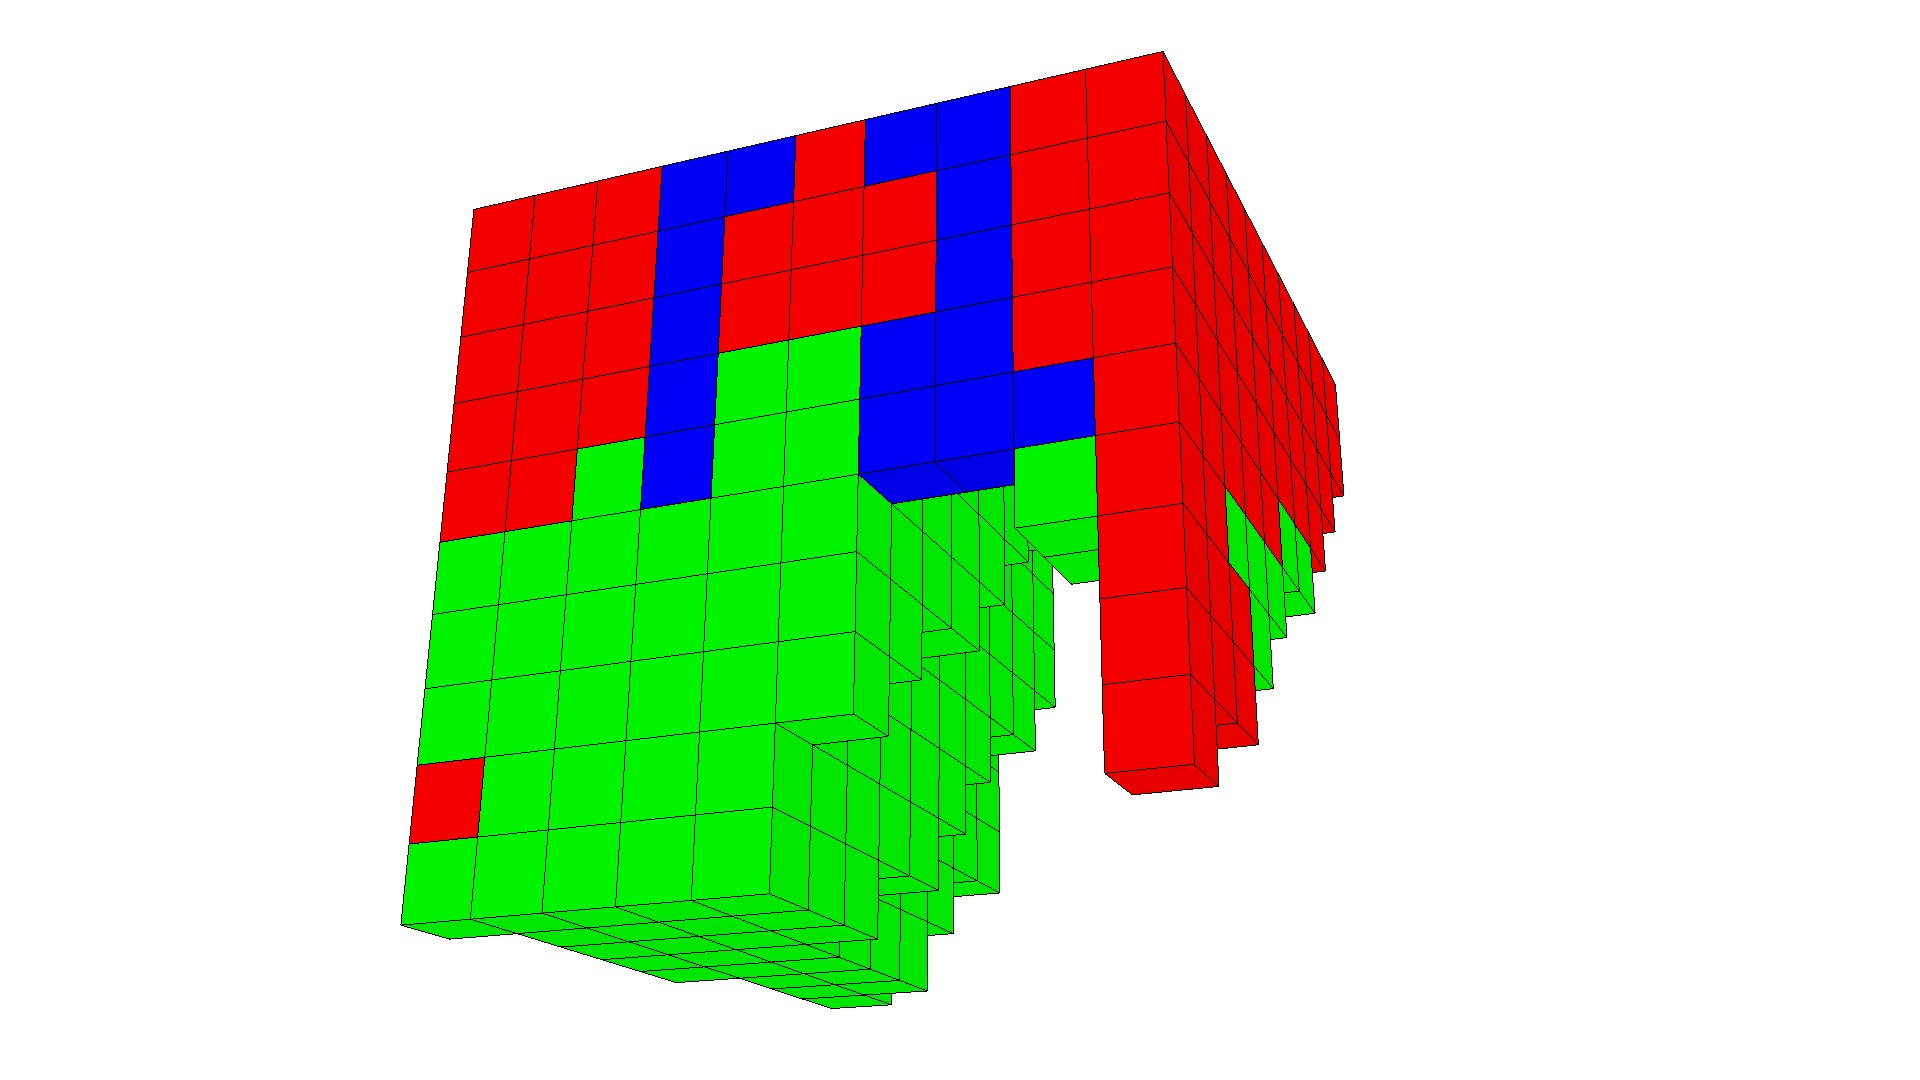
\includegraphics[width=0.19\textwidth]{../Figures/Robots/f_4_g_1000.jpg}
\caption{Fitness based search}
\end{subfigure}\\
\begin{subfigure}[b]{1.0\textwidth}
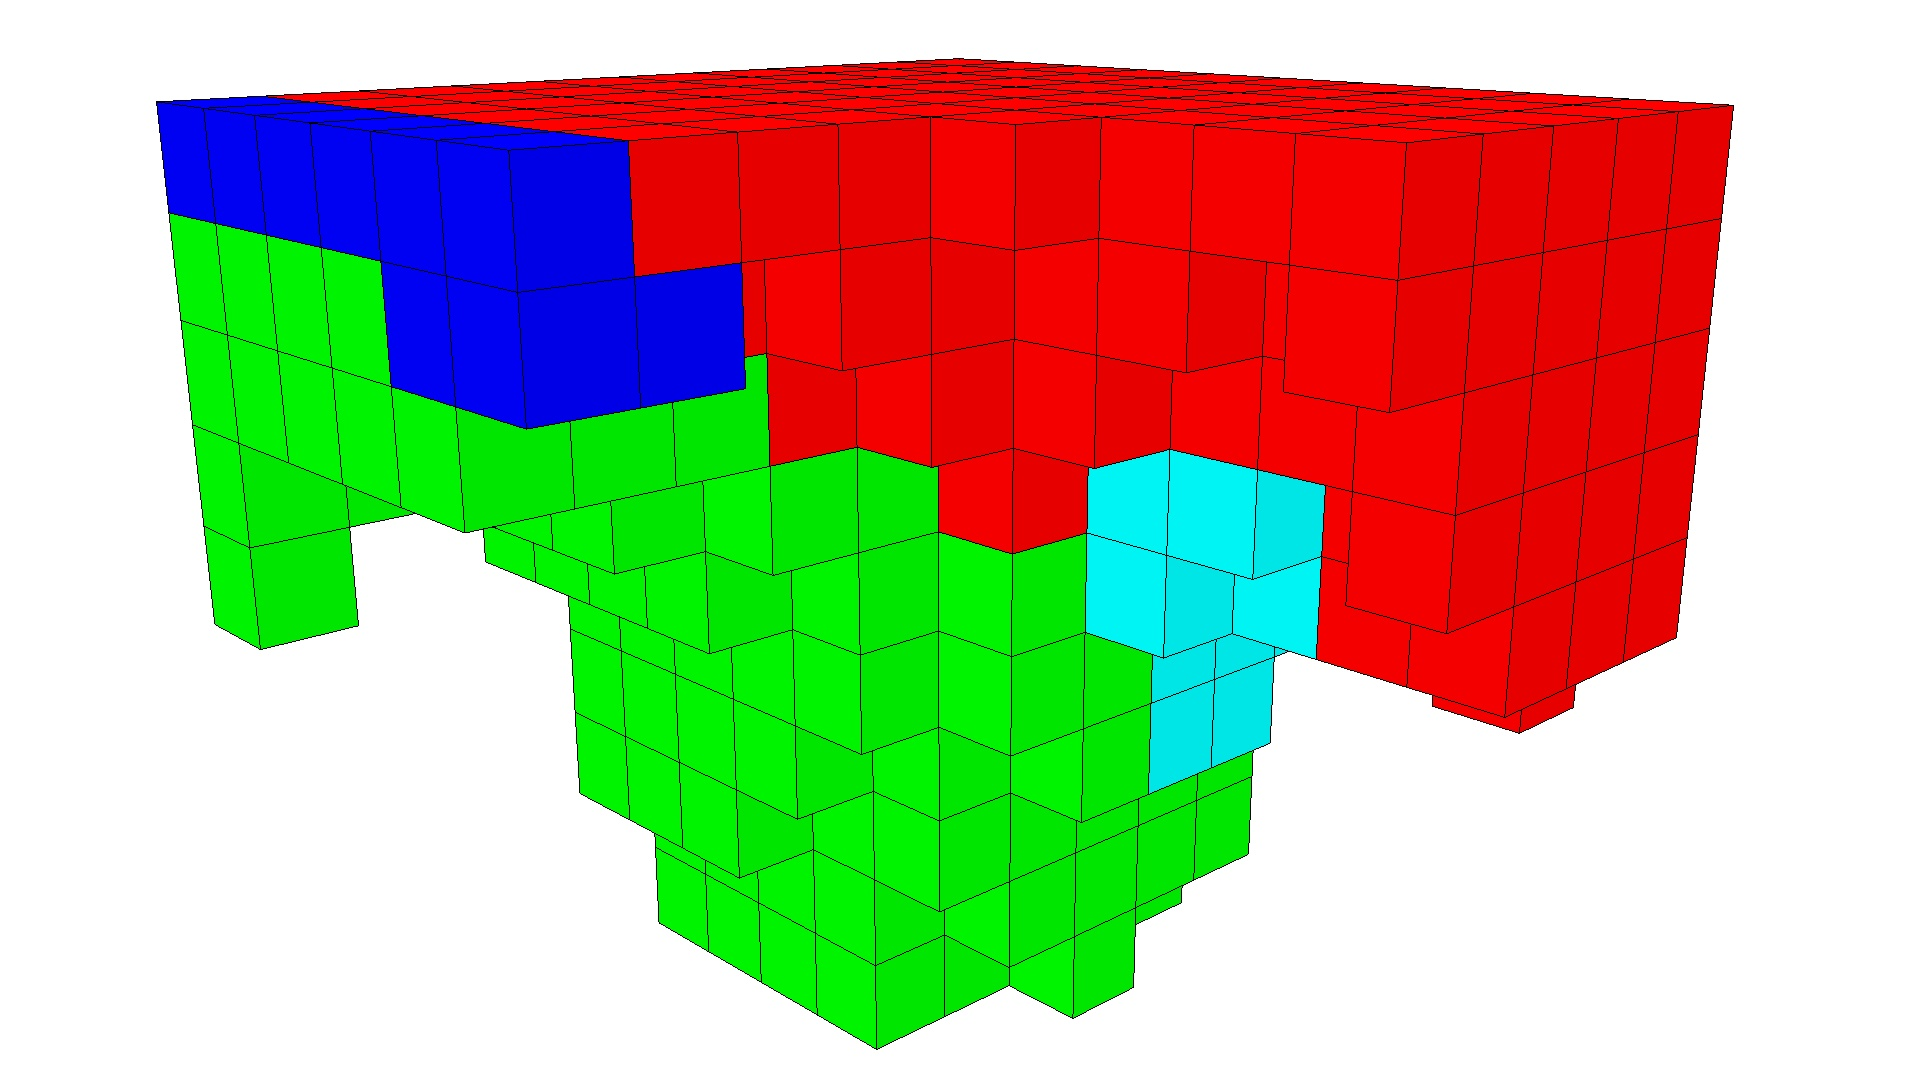
\includegraphics[width=0.19\textwidth]{../Figures/Robots/n_4_g_100.jpg}
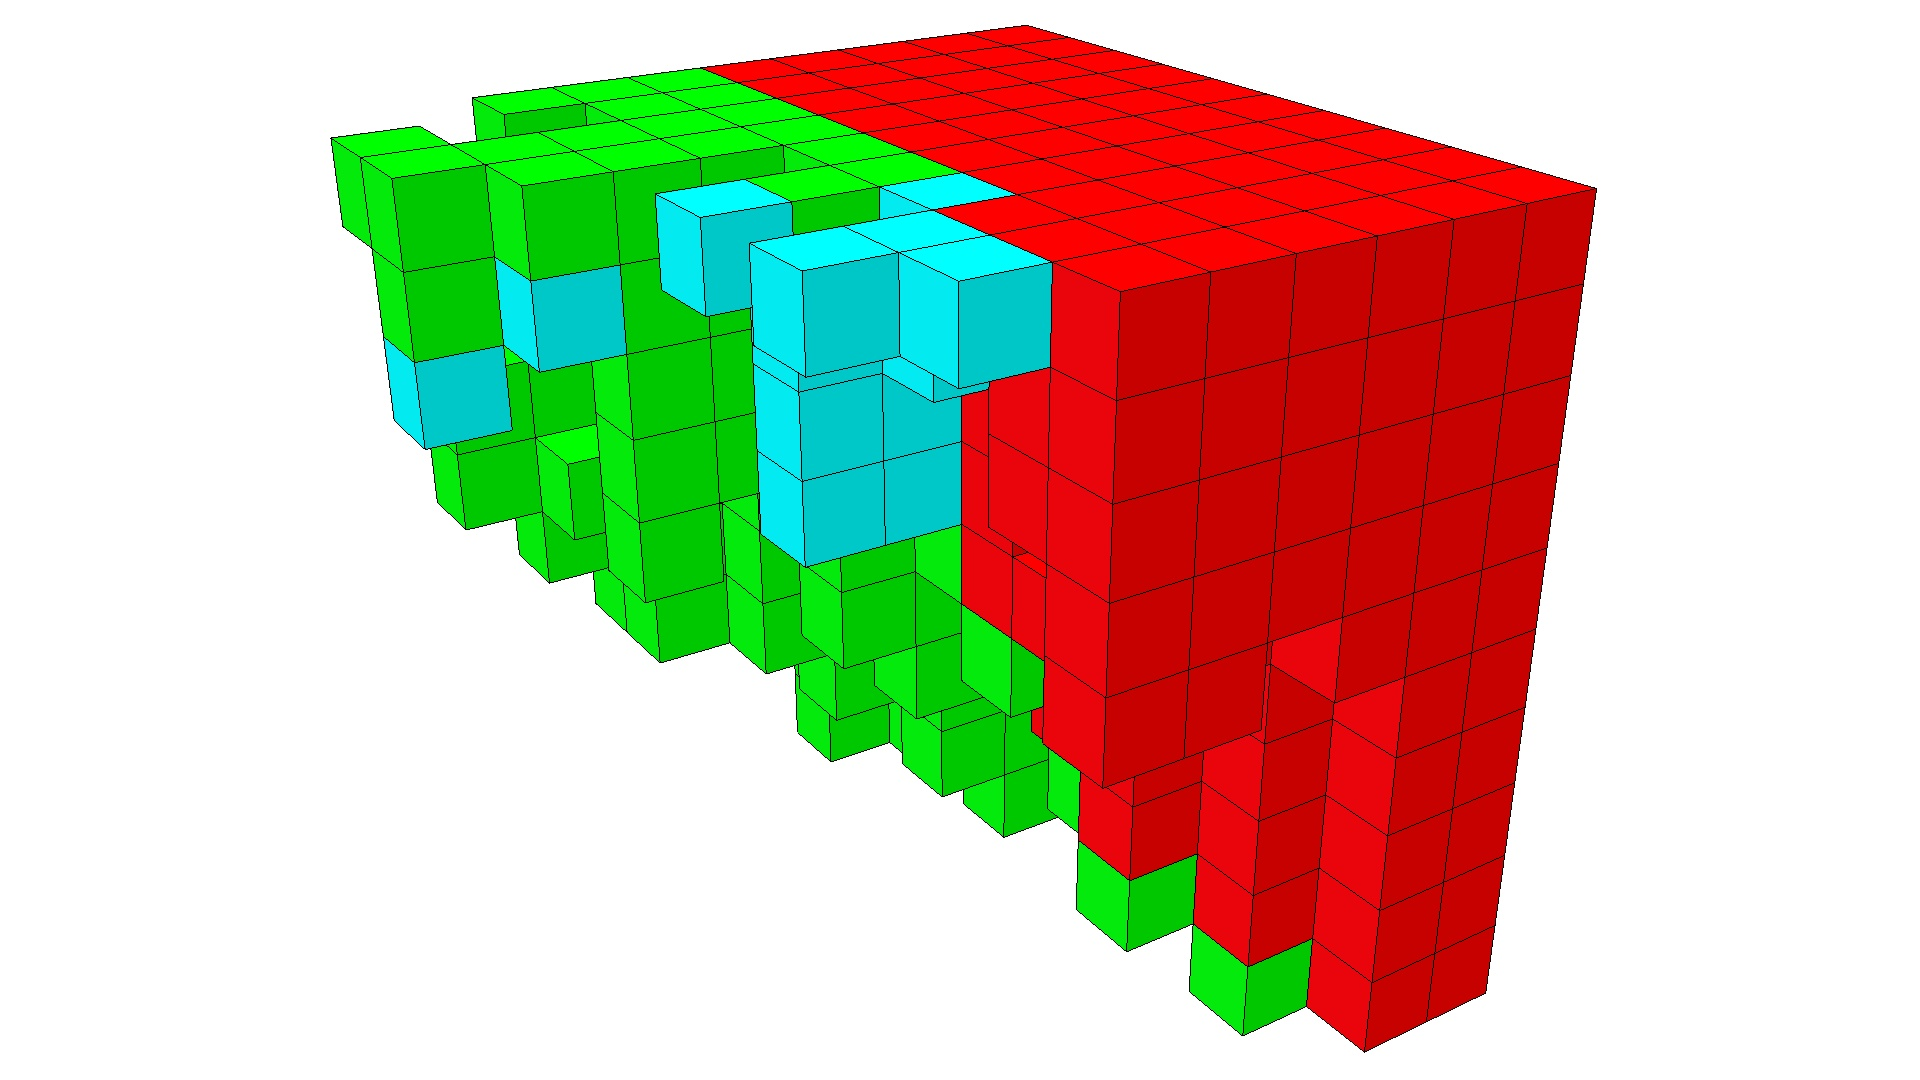
\includegraphics[width=0.19\textwidth]{../Figures/Robots/n_4_g_200.jpg}
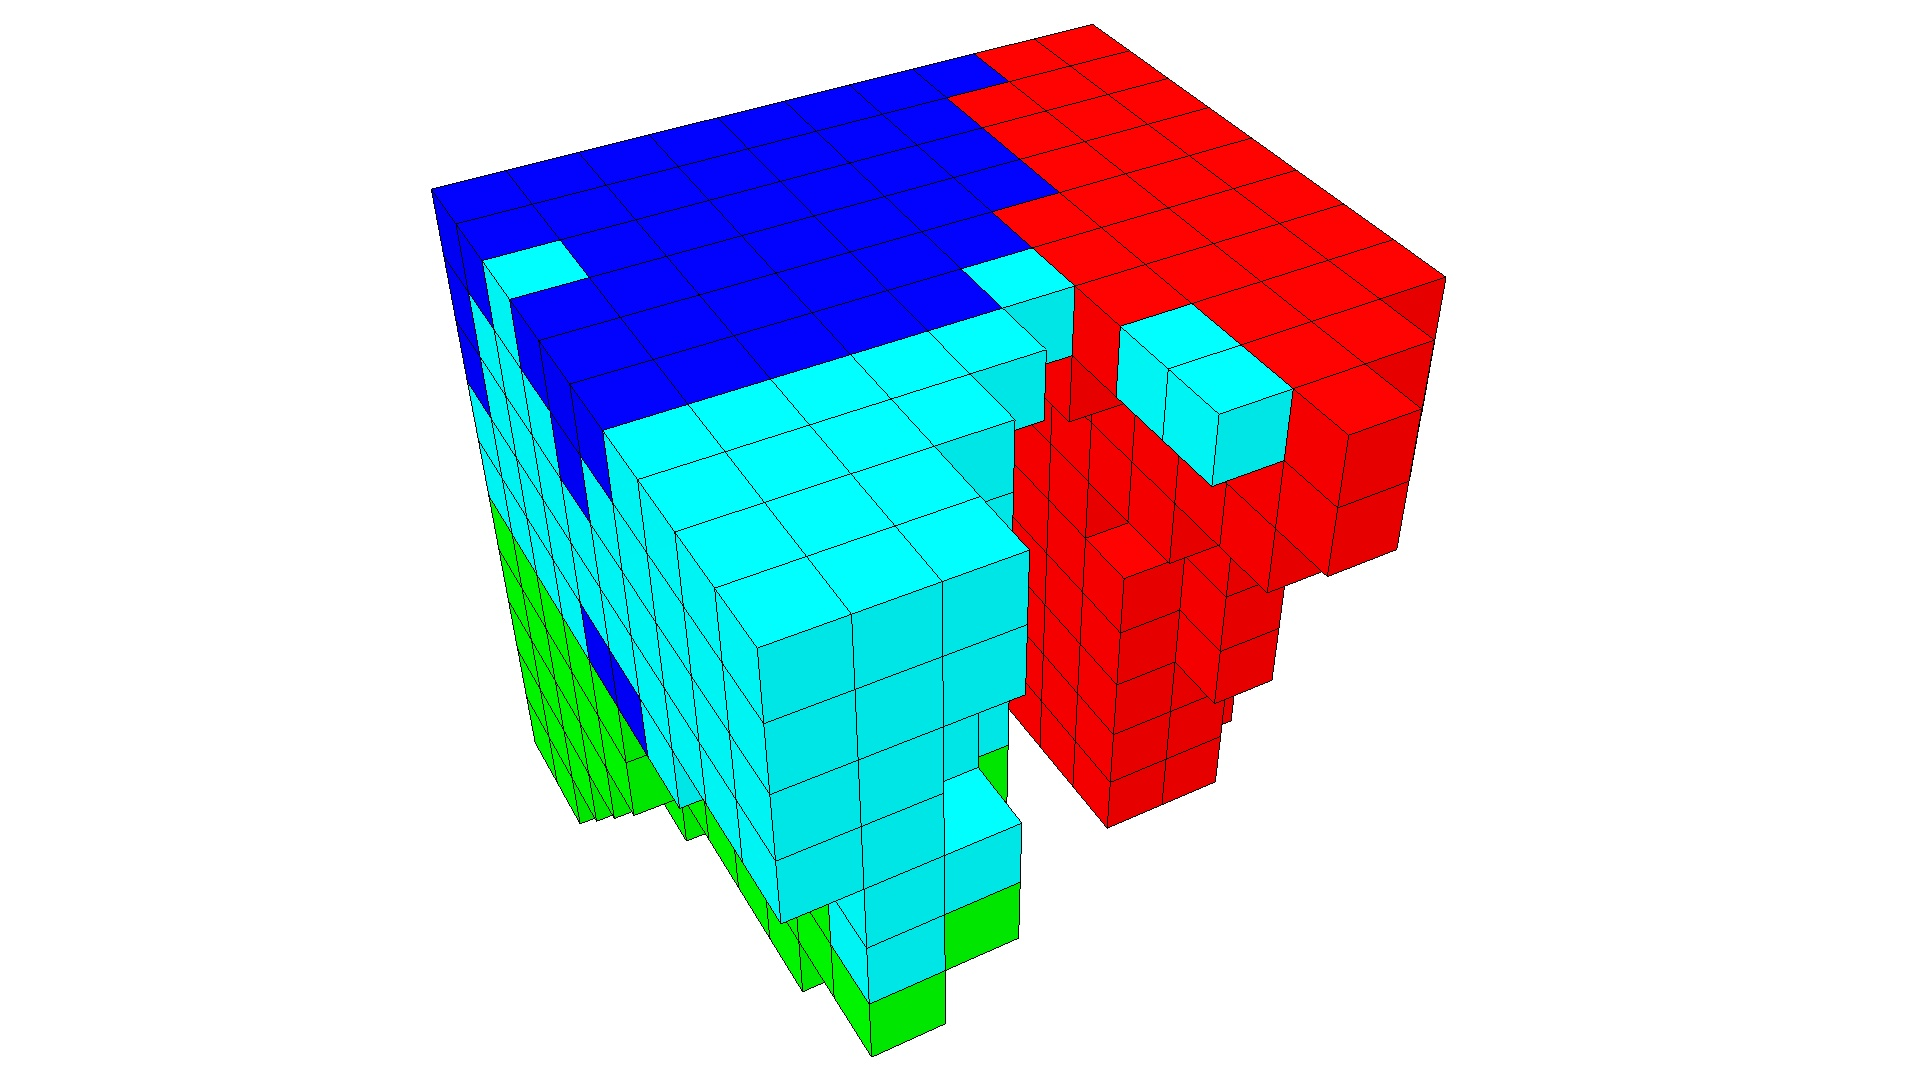
\includegraphics[width=0.19\textwidth]{../Figures/Robots/n_4_g_300.jpg}
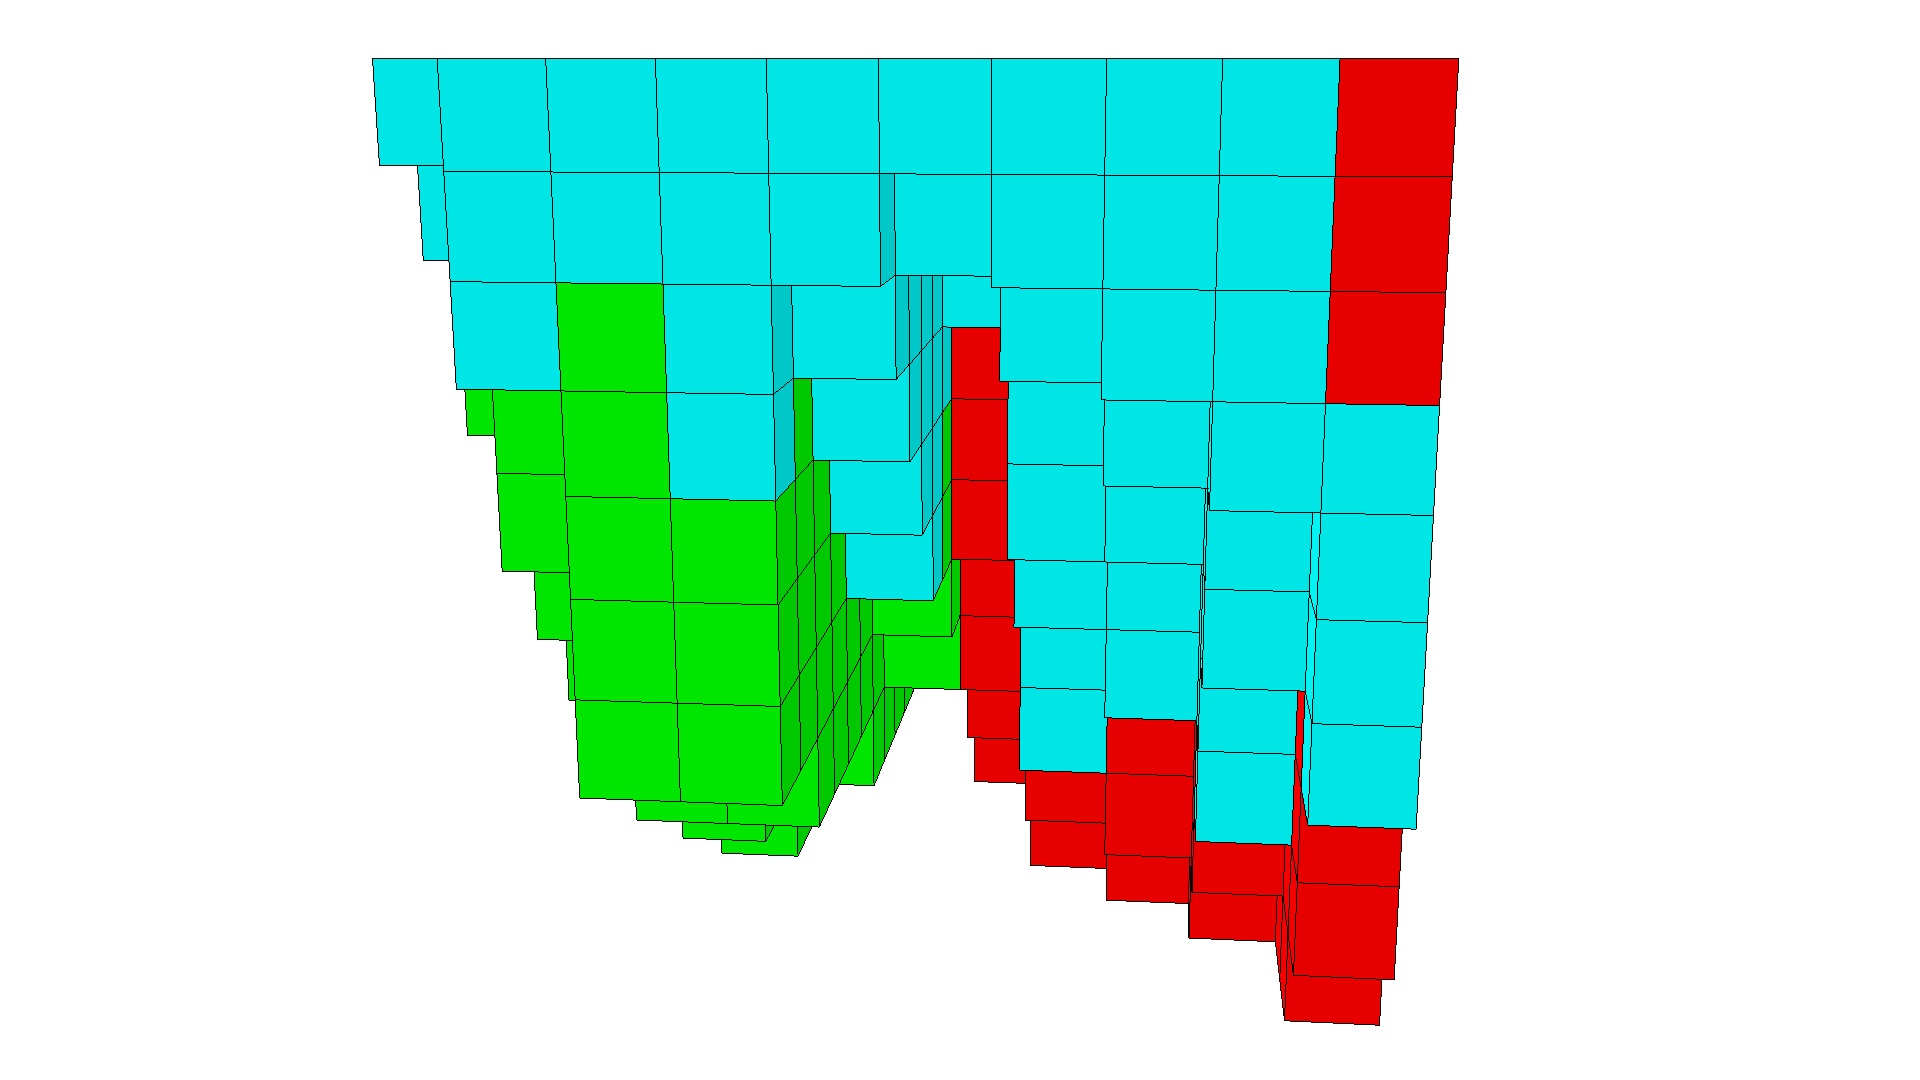
\includegraphics[width=0.19\textwidth]{../Figures/Robots/n_4_g_400.jpg}
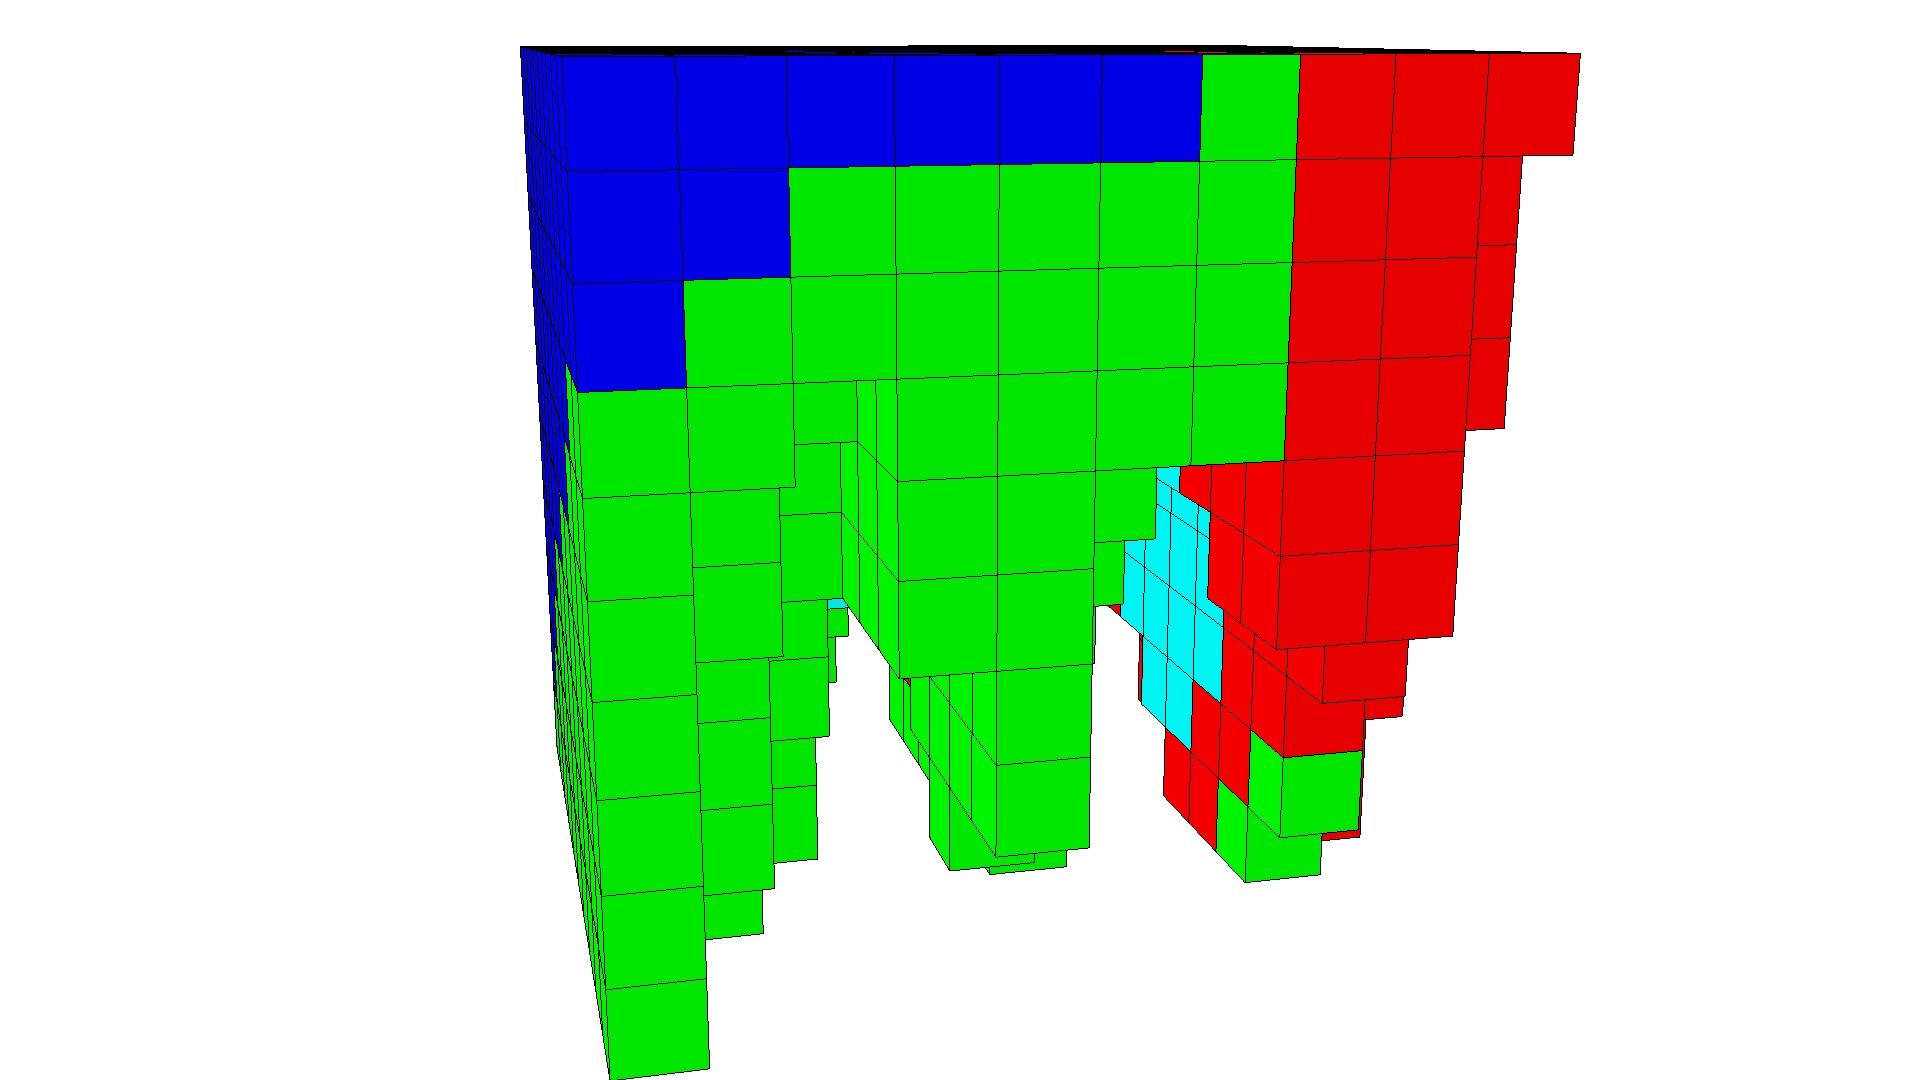
\includegraphics[width=0.19\textwidth]{../Figures/Robots/n_4_g_500.jpg}\\
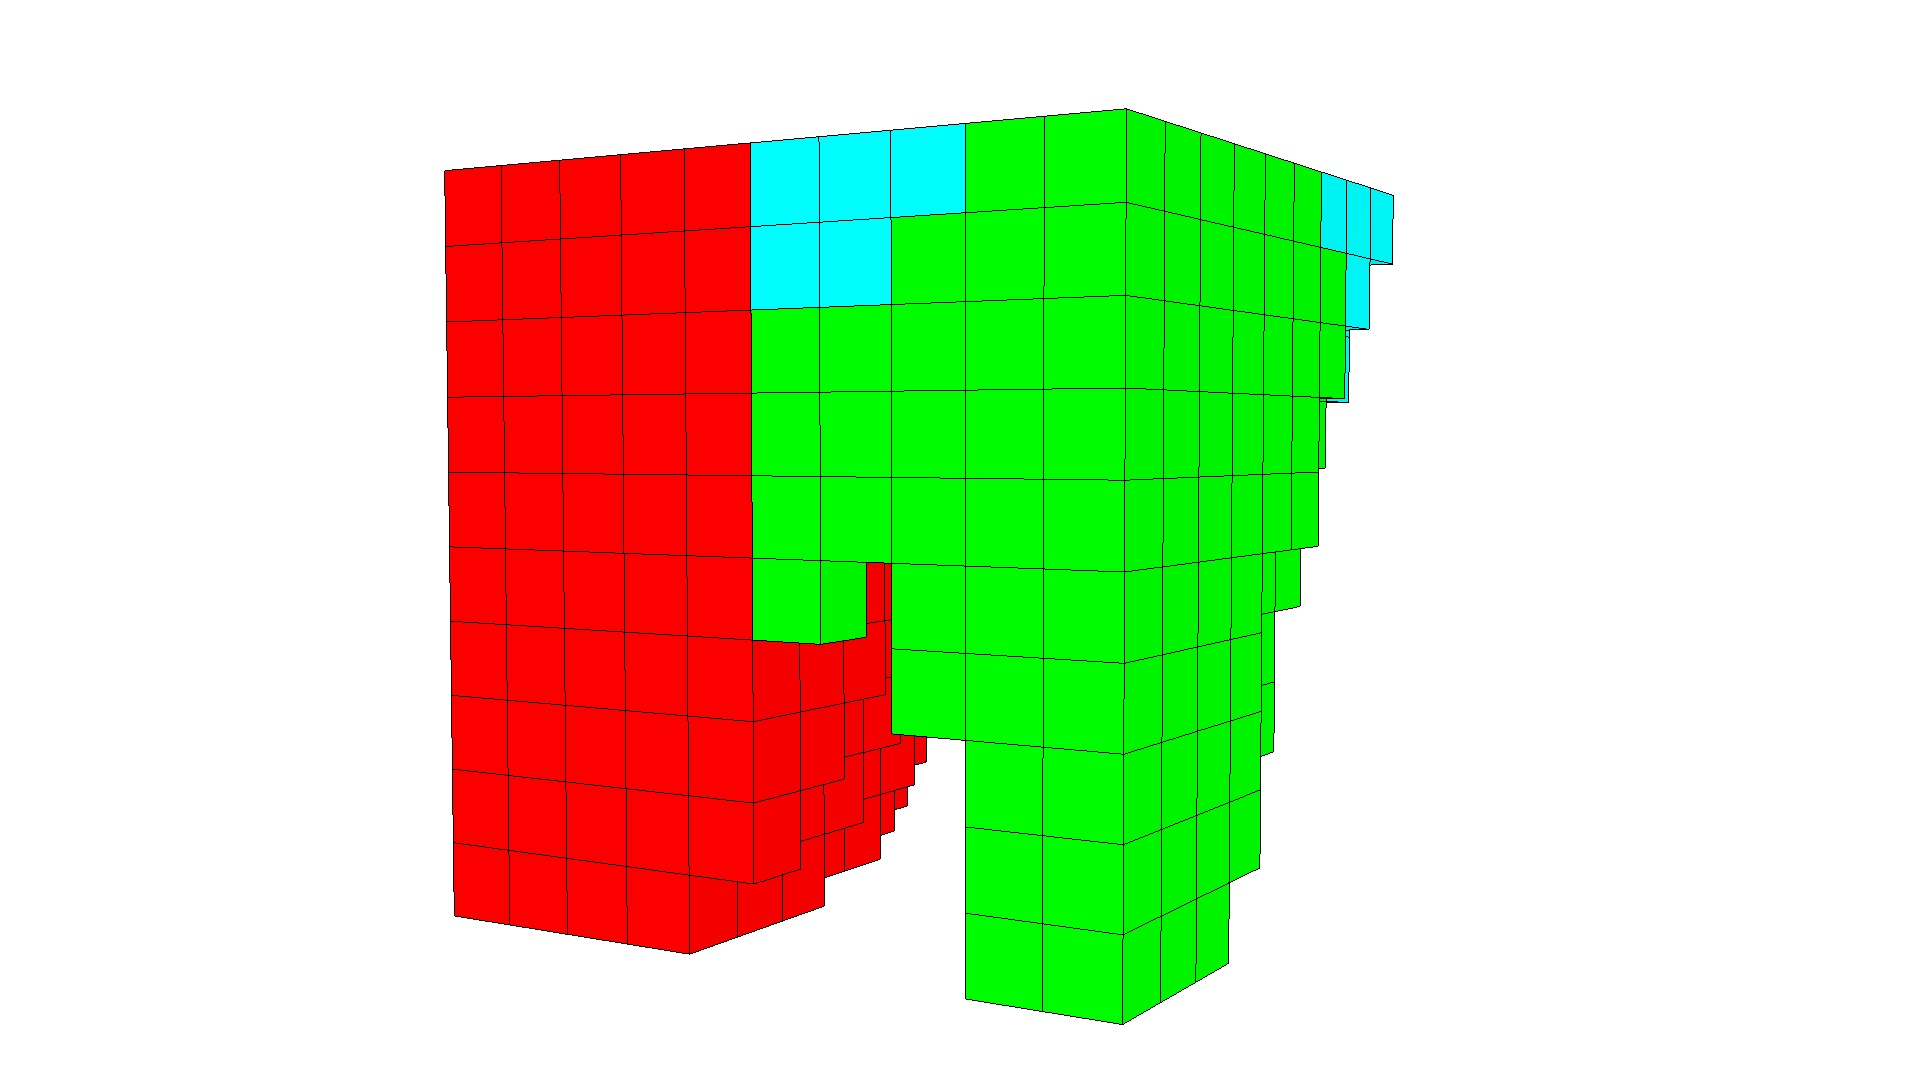
\includegraphics[width=0.19\textwidth]{../Figures/Robots/n_4_g_600.jpg}
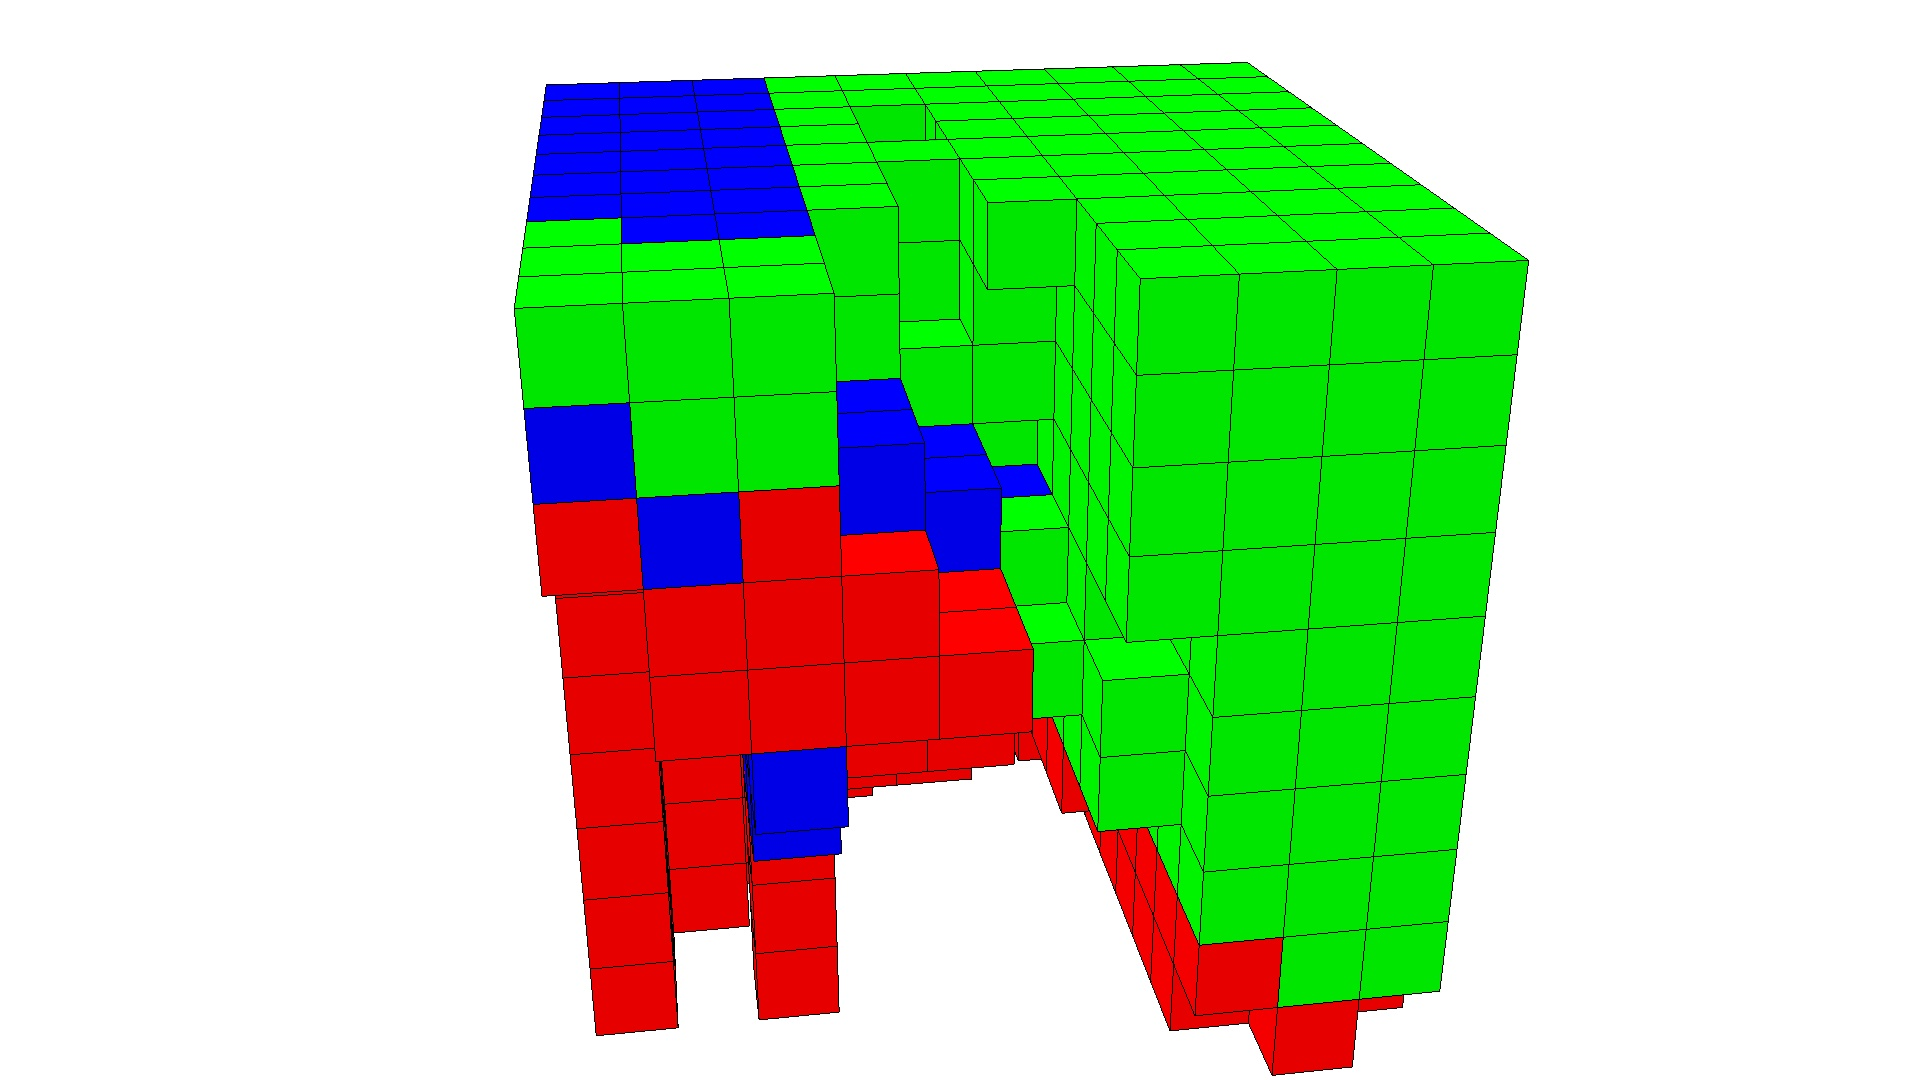
\includegraphics[width=0.19\textwidth]{../Figures/Robots/n_4_g_700.jpg}
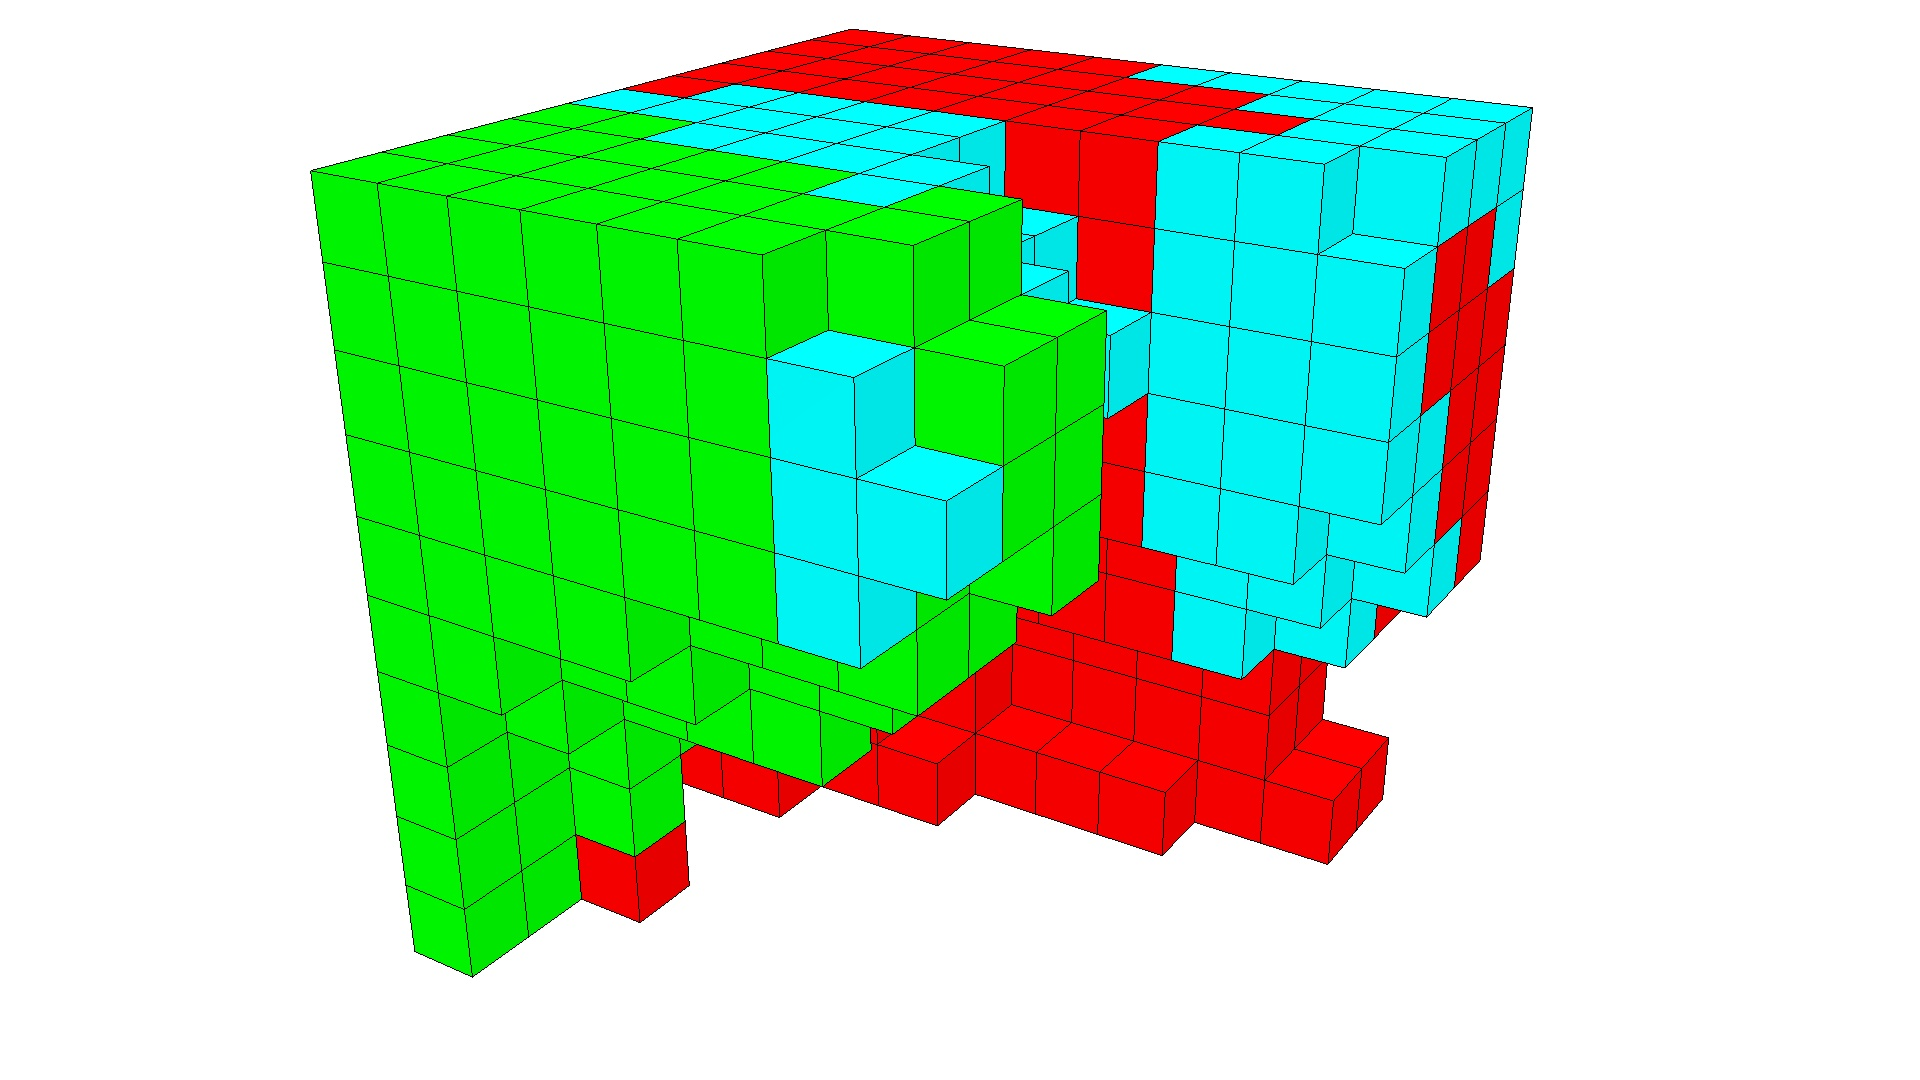
\includegraphics[width=0.19\textwidth]{../Figures/Robots/n_4_g_800.jpg}
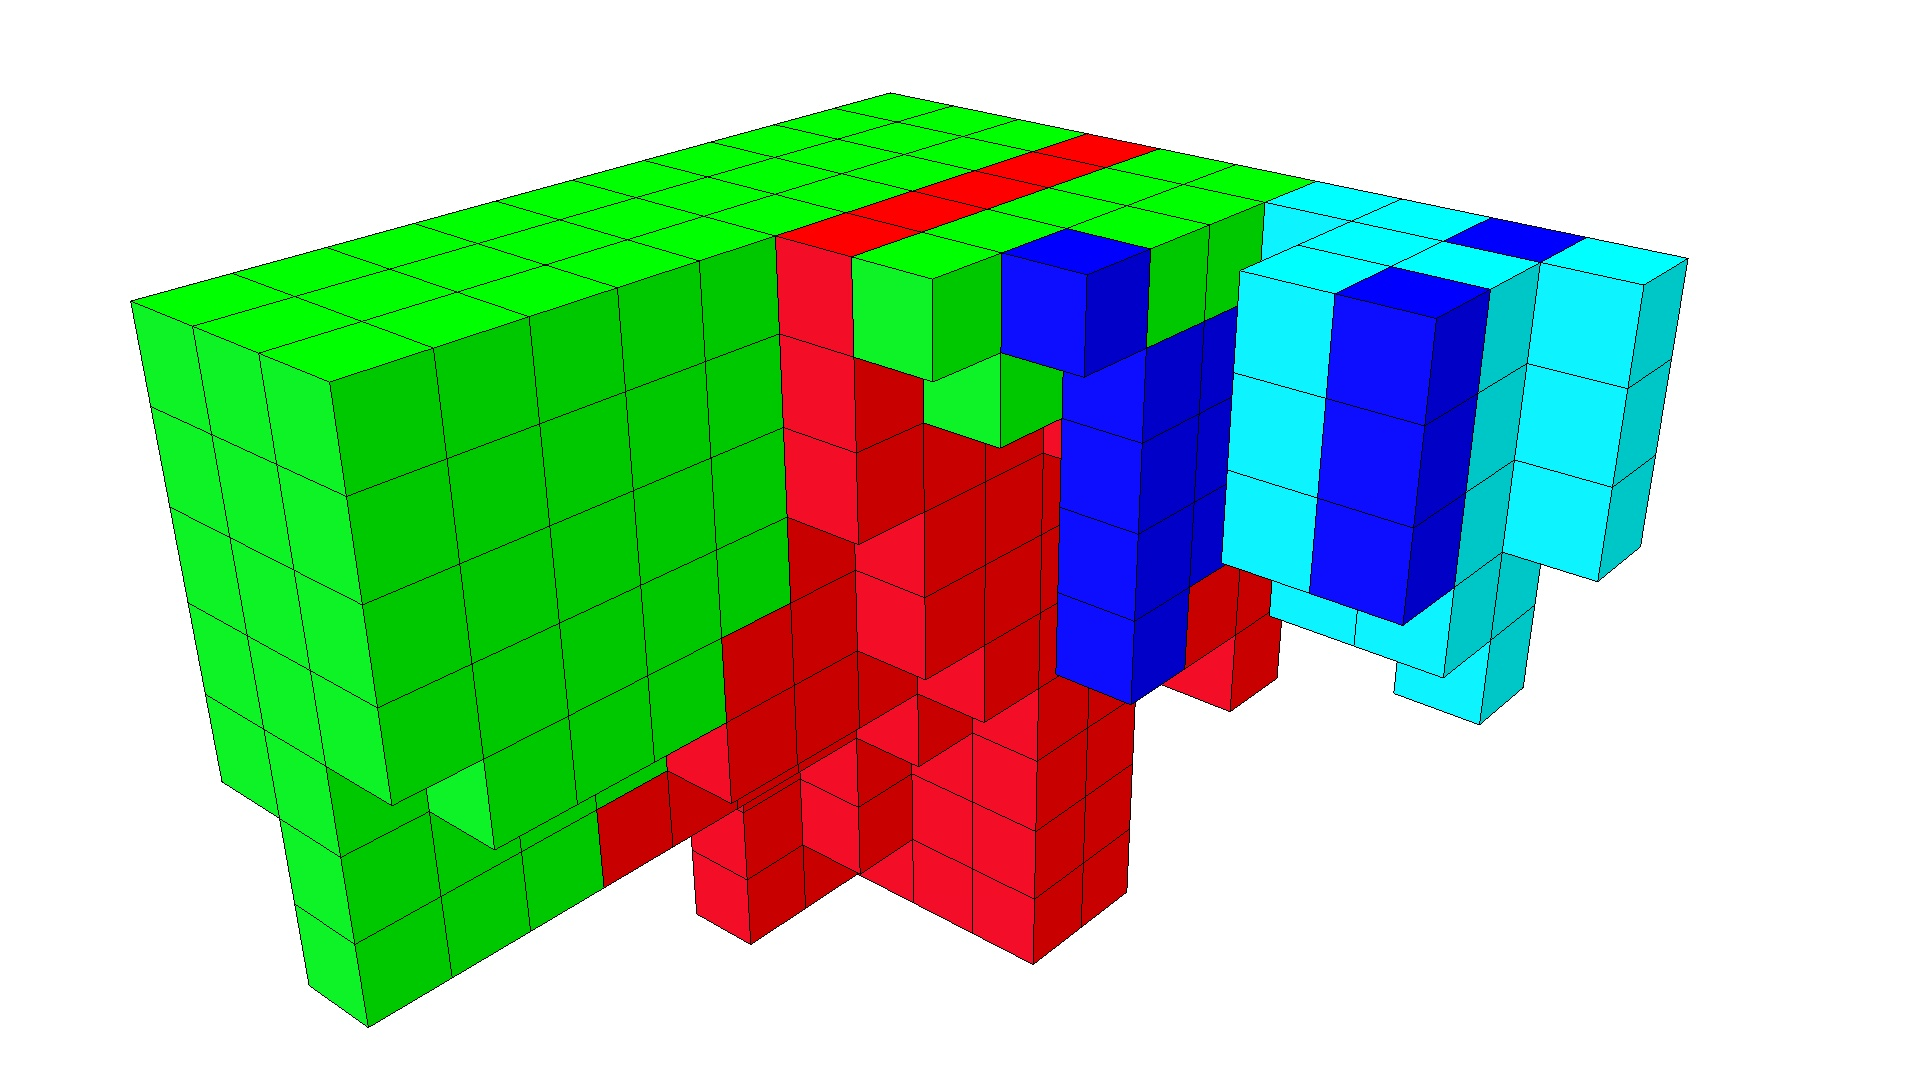
\includegraphics[width=0.19\textwidth]{../Figures/Robots/n_4_g_900.jpg}
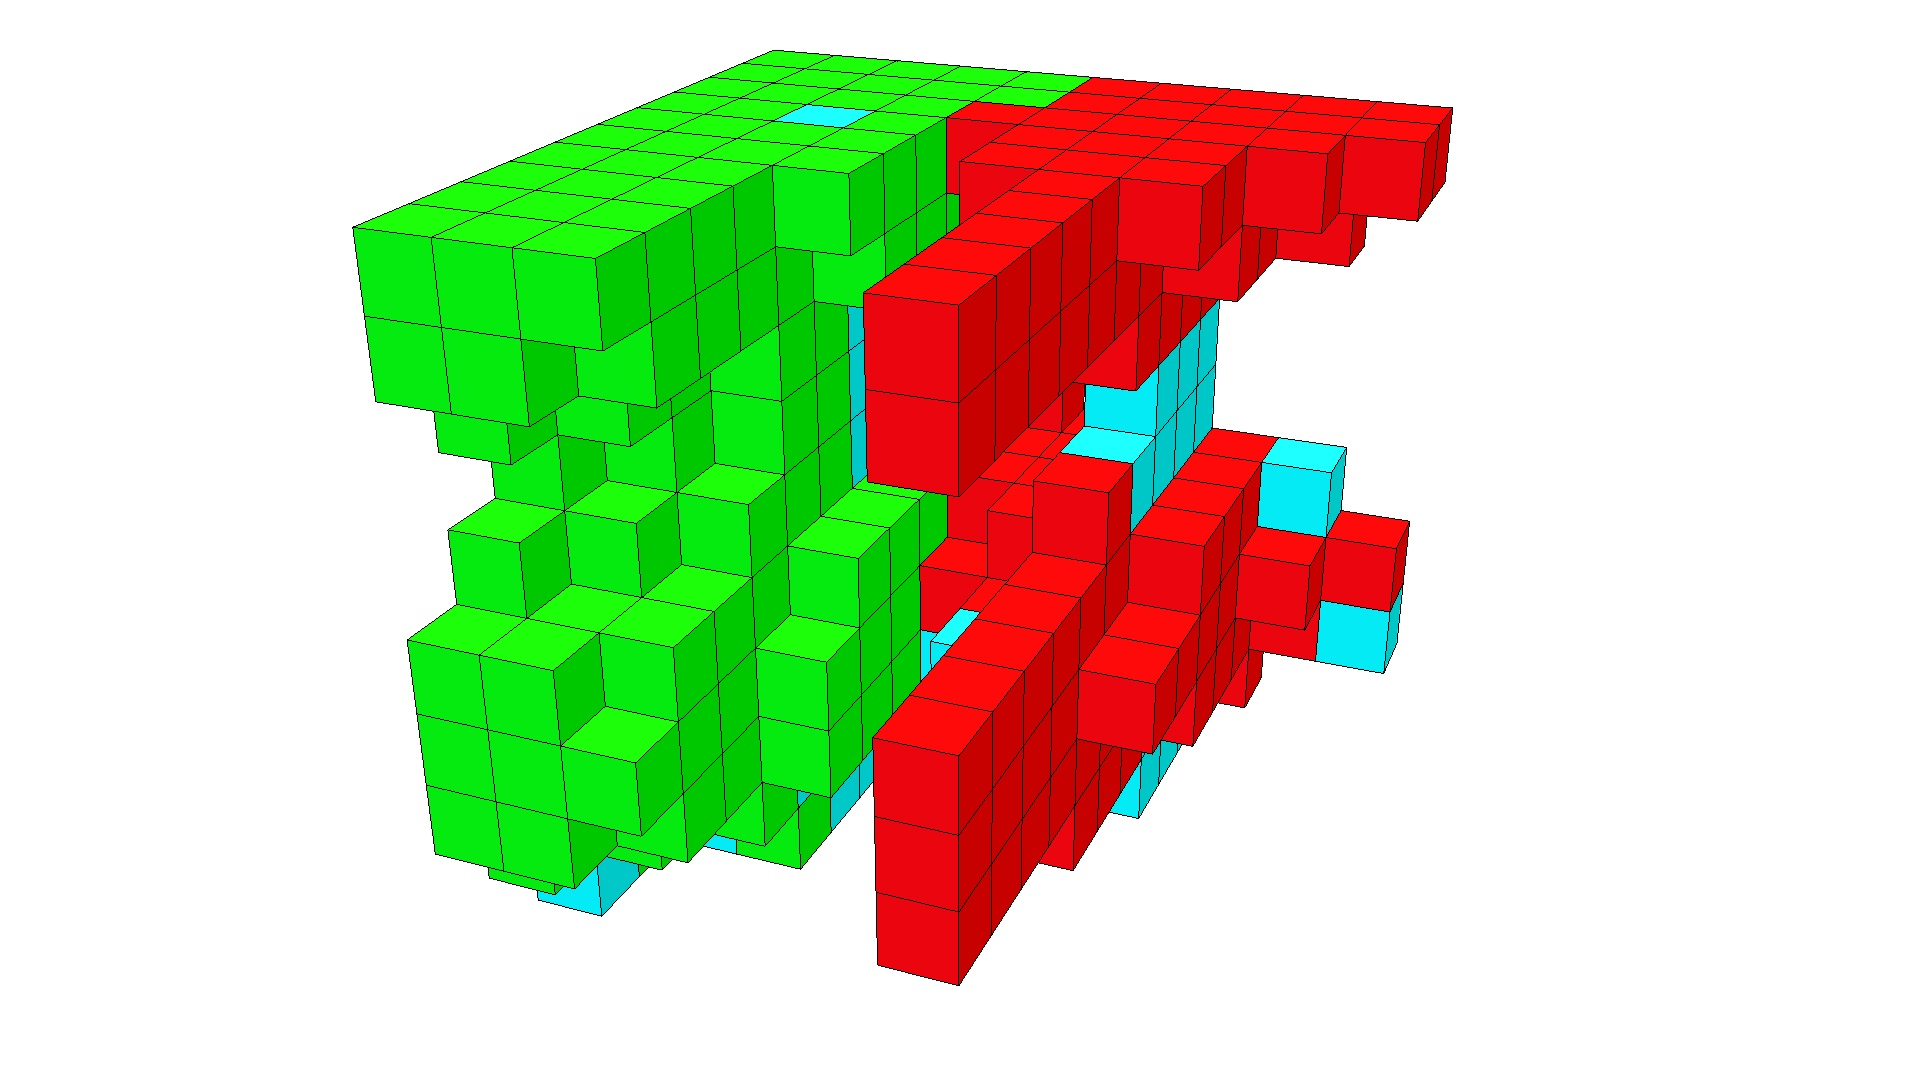
\includegraphics[width=0.19\textwidth]{../Figures/Robots/n_4_g_1000.jpg}
\caption{Novelty search}
\end{subfigure}
\caption{Fitness based search trying to optimize a specific structure while the search for novelty results in a variety of shapes. (Settings~\ref{Settings-size10})}
\label{fig:morphologies}
\end{figure}


\subsection{Diversity of Individuals in \emph{Novelty}-Search}

The gain in performance that novelty search achieved over fitness-based search has been discussed in detail.  At the same time evolved morphologies illustrated earlier showed that both methods can create morphologies that are able of efficient locomotion. The diversity of the individuals in the behavior space verified how novelty search can achieve the gain in the objective measure by seeking for novel behaviors. What is missing, is what happens in the morphology of the soft-robots during the evolution. Figure~\ref{fig:morphologies}, shows the champions every hundred generations of an experimental run for novelty and fitness-based search. While the fitness-based search is stuck trying to optimize a specific morphology of a soft robot, novelty search is searching the behavior space unveiling new morphologies. The same motif appears in every independent run of fitness and novelty search. Novelty search evolves a larger variety of morphologies, whereas fitness-based evolution is sticking to certain shapes, different in every run. Both search techniques have their advantages and disadvantages. First, fitness-based search optimizes (optimized distribution of materials within the structure) certain shapes during the evolution,while novelty search does not optimize them. Novelty search allows the evolution of highly novel behaviors-morphologies. These novel morphologies even in cases that they perform well under a task will never have the time to be improved. During the next sections of this chapter, ways of combining both search methods' merits are discussed.

\begin{figure}[t!]
\centering
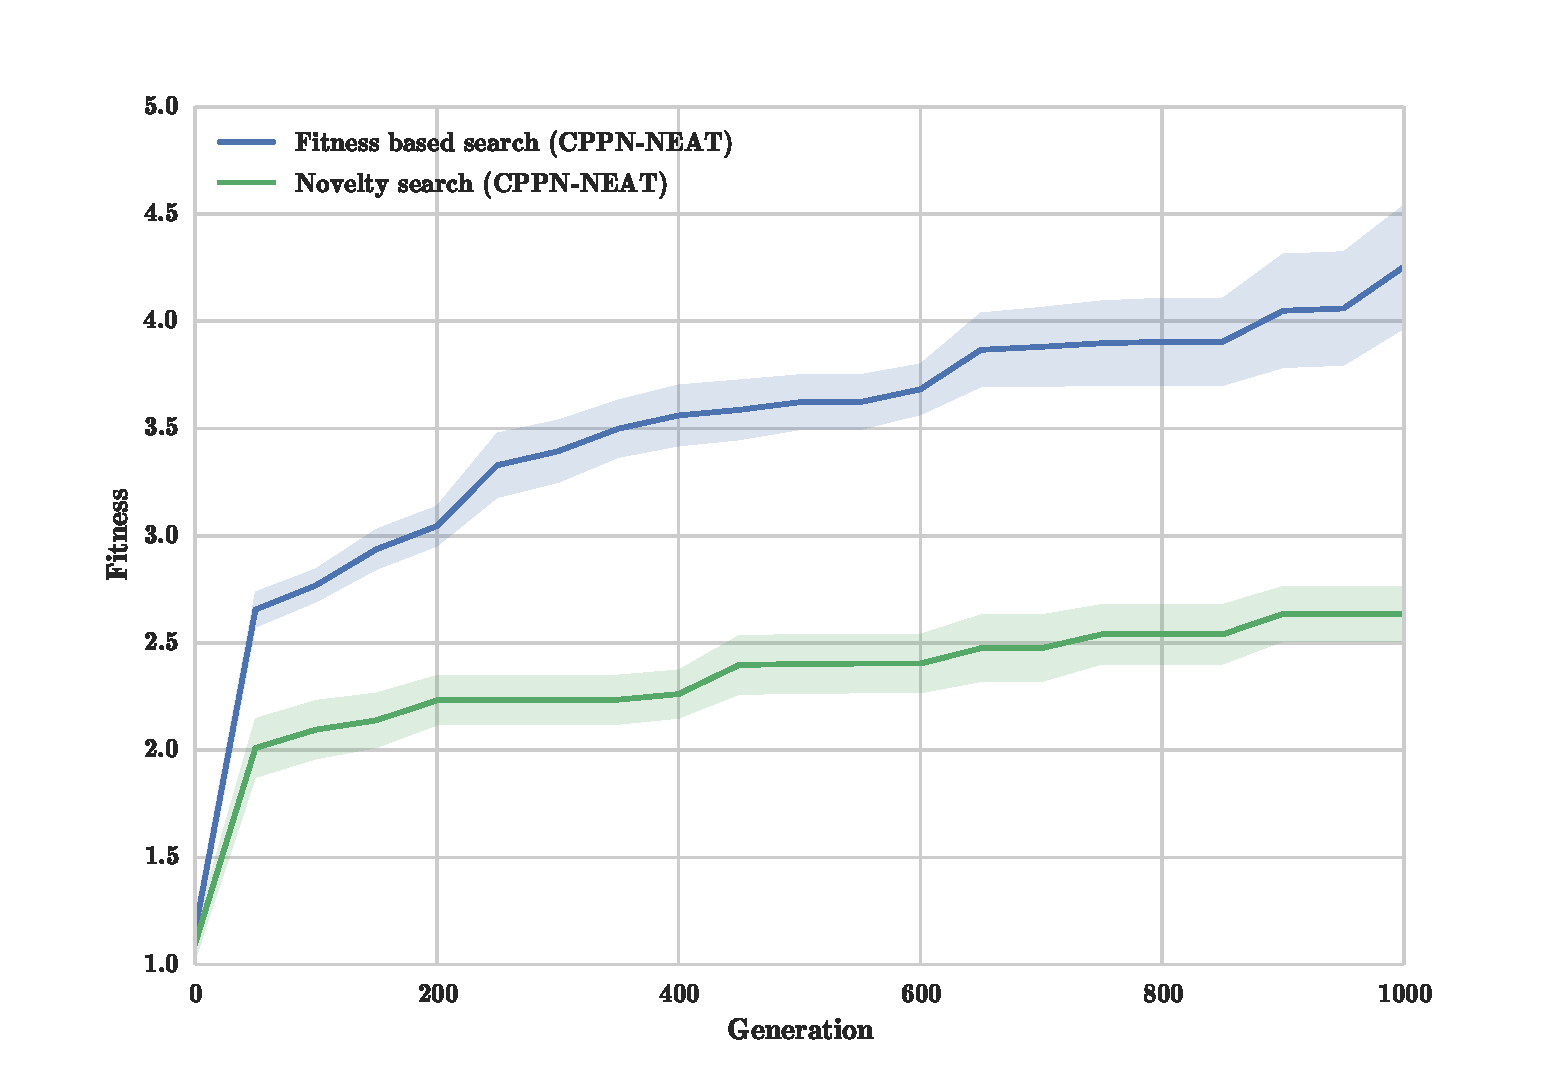
\includegraphics[width=1.0\textwidth]{../Figures/Results/FitNovSize5Pen2.pdf}
\caption[]{Best so far fitness averaged over $10$ runs, penalizing actuated materials for \emph{fitness} - \emph{novelty} search with generative encoding. (Settings~\ref{Settings-size5})}
\label{fig:FitNovSize5Pen2}
\end{figure}

\subsection{How Behavior Selection Affects \emph{Novelty}-Search}

In novelty search, a good behavior metric to measure novelty should contain information about the objective function. In the case of evolving the gait of soft-robots, trajectories can be highly informative regarding the displacement of the robot's body, as well as, the locomotion strategy that is observed. Two soft-robot bodies which traveled the same distance within an equal time horizon, should have the same fitness if displacement is only measured. Nevertheless, most objective functions used in the evolution of robot-gait cannot describe the locomotion strategy produced by the robot controller. The observed behavior of a robot can contain this information. Novelty search can take advantage of a descriptive behavior metric. Forcing the evolution to seek for  novel solutions in the behavior space, can result in the evolution of $>10 \times$ more novel behaviors than fitness-based search (depending on the threshold and the behavior metric) (see Fig.~\ref{fig:novelIndividualsFitNovComp}). This indirectly implies that fit individuals will be found as the behavior space is heavily searched. The importance of the behavior metric in novelty search is crucial in order fit solutions to be evolved within novel solutions of the behavior space defined. Two dimensional trajectories in the evolution of fast soft-robots, contain all the information needed to determine the fitness (speed). This metric is incorporated inside the behavior (trajectories) assuming constant sampling rate of the trajectories. To investigate the performance of novelty-search when no information about fitness is provided by the behavior, an objective function is selected that two-dimensional trajectories do not contain information about. The objective function is a penalized version\footnotemark of the displacement of the soft-robots in respect to the number of actuated (active) voxels in the soft-robot. Figure~\ref{fig:FitNovSize5Pen2}, illustrates the best so far fitness for both novelty and fitness-based search averaged on $10$ evolution runs. Comparing the results with Figure~\ref{fig:FitNovRandomDirectSize5} novelty search performs poorly in regards to the evaluation metric., whilst the same method outperforms traditional fitness-based search when the whole information of the fitness function is incorporated into the behavior. Trying to find novel trajectories in the first case is proved successful in respect to the final displacement of the individuals are evolved. On the other hand, trying to optimize the distance that soft-robots traveled and at the same time minimize the number of actuated voxels, proved crucial in the performance of novelty search. As it is shown, the performance of novelty search depends heavily on the selection of the behavior metric.
\footnotetext{Actuated materials penalize fitness: \[f = (1 - (n_{actuated} / n_{total})^{1.5}) \times disp \], where $n_{actuated}$, is the number of actuated voxels, $n_{total}$ total number of voxels and $disp$ the displacement of the softbot's center of mass.}


\begin{figure}[t!]
\centering
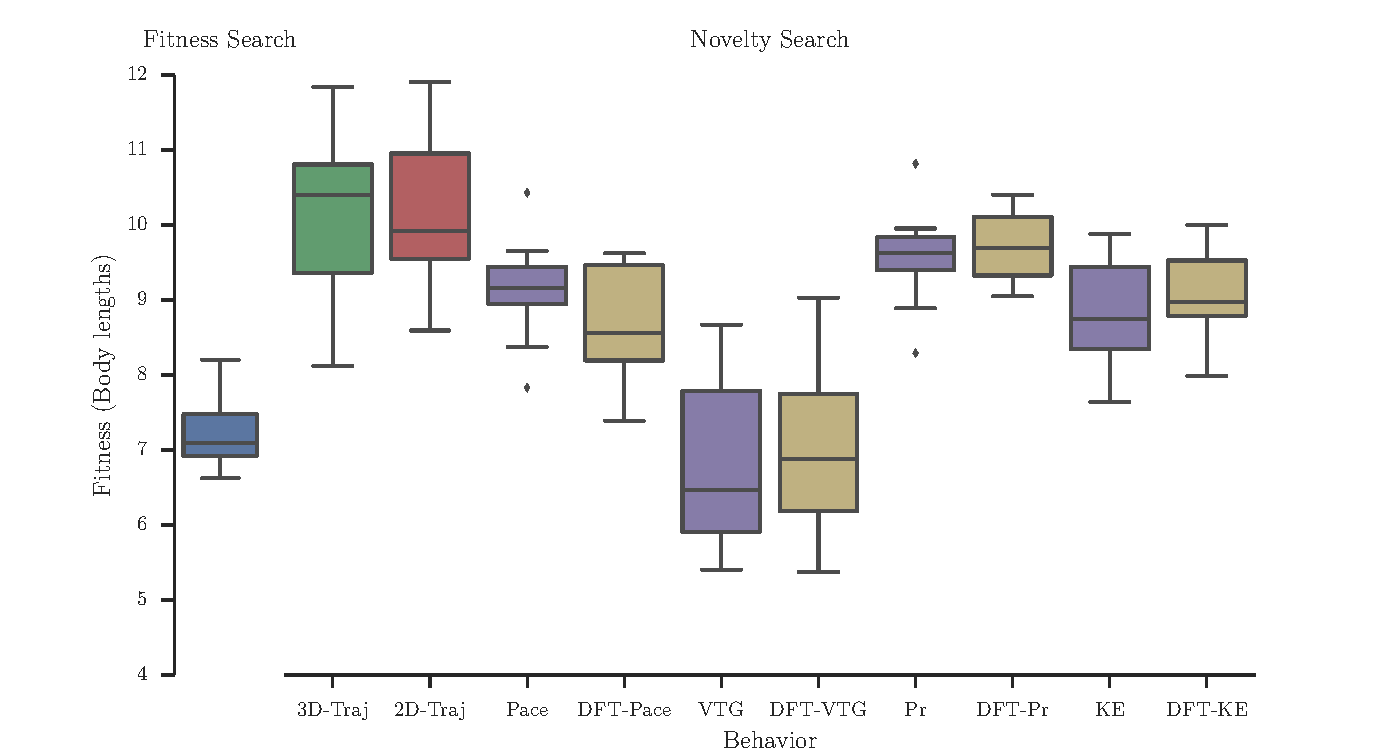
\includegraphics[width=1.0\textwidth]{../Figures/Results/BehaviorsPerformance.pdf}
\caption{Comparison of the evolution's best fitness result from $10$-runs under different behavioral metrics for \emph{novelty} search (right). \emph{Fitness} search is also evaluated under the same settings (left - \textcolor{MidnightBlue}{blue} box). (Settings~\ref{Settings-size7})}
\label{fig:BehaviorsPerformance}
\end{figure}

To verify the previous finding, where novelty search failed to compete with fitness-based search when the behavior metric used did not contain information about the objective function defined, a set of behavior metrics have been used. Figure~\ref{fig:BehaviorsPerformance} illustrates the performance achieved by novelty search, for all behaviors defined in Table~\ref{Behaviors}. In addition, the performance of fitness-based search is presented in the left side of the figure (\textcolor{NavyBlue}{blue} box).

A set of $10$ behavior metrics are used including the three dimensional trajectories of the soft robots (3D-Traj), the two dimensional projection on $x,y$-axes of the previous behavior (2D-Traj), the pace of the soft-robots sampled every $0.001$ sec. (Pace), the discrete Fourier transformation of the same signal which is sampled every $0.00001$ sec. (DFT-Pace), the number of voxels touching the ground on each sampling time-step (VTG, DFT-VTG), the maximum pressure per time-step (Pr, DFT-Pr), and the kinetic energy of the whole structure (KE, DFT-KE). What is shown here, is the fitness in body lengths of the champion soft-robot of the whole evolution from $10$-independent runs of the experiment. Both trajectory-type behaviors achieve the best performance in regards to the fitness measured. The distribution of champion fitness novelty search achieved with the two-dimensional trajectories shows a small difference in favor of two-dimensional over three-dimensional trajectories. The third highest performance is achieved by the maximum pressure behavior, which is close to the previous two trajectory-type behaviors. Pace and kinetic energy of the soft-robots are the next best behavior-types in the performance ladder. The worst behavior metric regarding the fitness that achieved is the number of voxels touching the ground.

The performance of novelty search when trajectories of the soft-robots are used as a behavior metric is superior over all other behavior metrics. Trajectories are a very good selection for this kind of evolution, since they can indirectly not only encode the objective function which is the displacement, but also the locomotion strategy. The reason why they achieve such a high performance is that novel behaviors in the space of trajectories result in long trajectories which can be described novel. The rest of the behavior metrics apart from VTG and VTG-DFT, are close, as far as the final performance of the evolution is concerned. One reason they fail to meet the trajectories' performance is the fact that even though they keep track of cues that can describe the performance of the robot (speed/displacement), they cannot encode the direction of them. Soft-robots having a circle trajectory can produce fast locomotion, in this case, the measured displacement from their initial position will remain low. Counting the number of voxels of a soft-robot that touch the ground in every sampling timestep of the simulation, does not imply how fast the robot is moving. A fast moving robot that is hopping can have a similar behavior with a hopping robot that stays in the same position after each jump. In the contrary, using the trajectories of these two soft-robots would have been highly variant. 

In the same figure (see Fig.~\ref{fig:BehaviorsPerformance}) and on the left side of it (\textcolor{MidnightBlue}{blue} box), fitness-based search is also evaluated under the same experimental settings. The performance of this objective optimization method is comparable only to the novelty search search when the voxels touching the ground are the selected behavior metric.

Apart from the effects of the behavior selection another aspect of novelty search, the sparsity equation is investigated in detail in Appendix~\ref{AdditionalExperiments}.




\begin{figure}[t!]
\centering
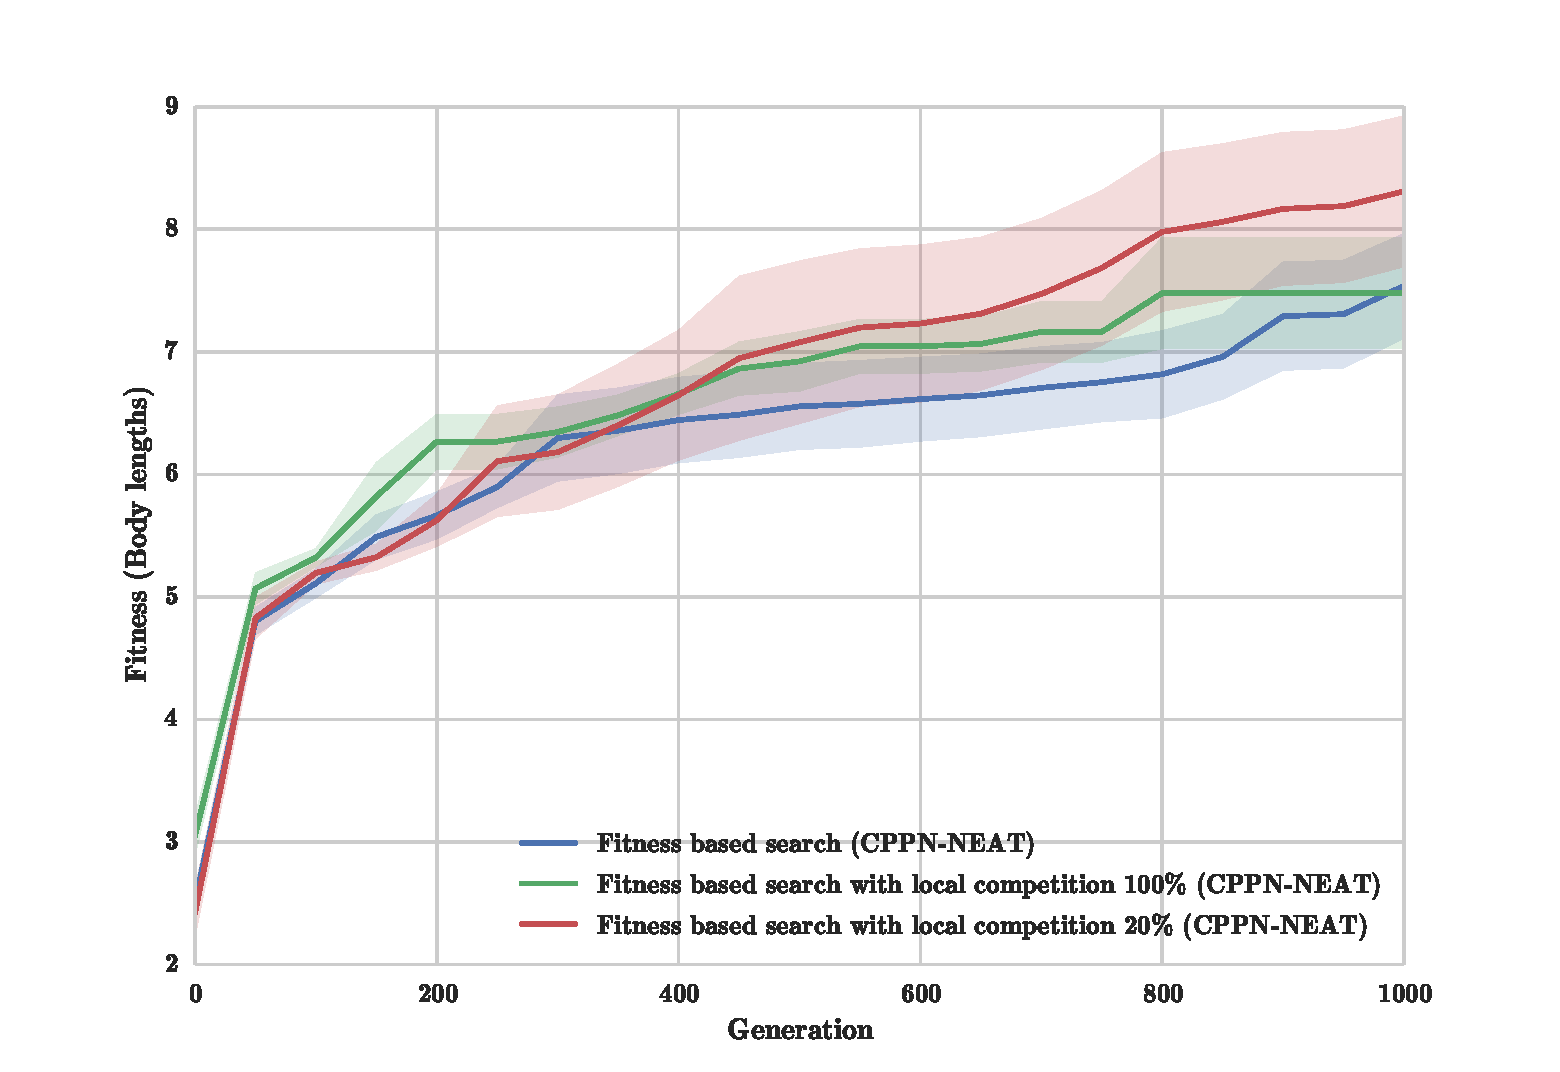
\includegraphics[width=1.0\textwidth]{../Figures/Results/fitComp100_20percent.pdf}
\caption{Best so far fitness averaged over $10$ runs, with no competition, local competition in the complete population of each species for \emph{fitness} search. (Settings~\ref{Settings-size7})}
\label{fig:fitComp100_20percent}
\end{figure}

\section{How Selection Affects the Performance of Both Search Methods}

Discussed extensively in previous Chapter (see Sec.~\ref{geneticAlgorithms}), selection is a process that picks individuals in order to breed, be mutated or be copied into the next generation. It is the part of any evolutionary algorithm that is responsible for producing the next generation, based on the individuals which exist into the current one.


\begin{figure}[t!]
\centering
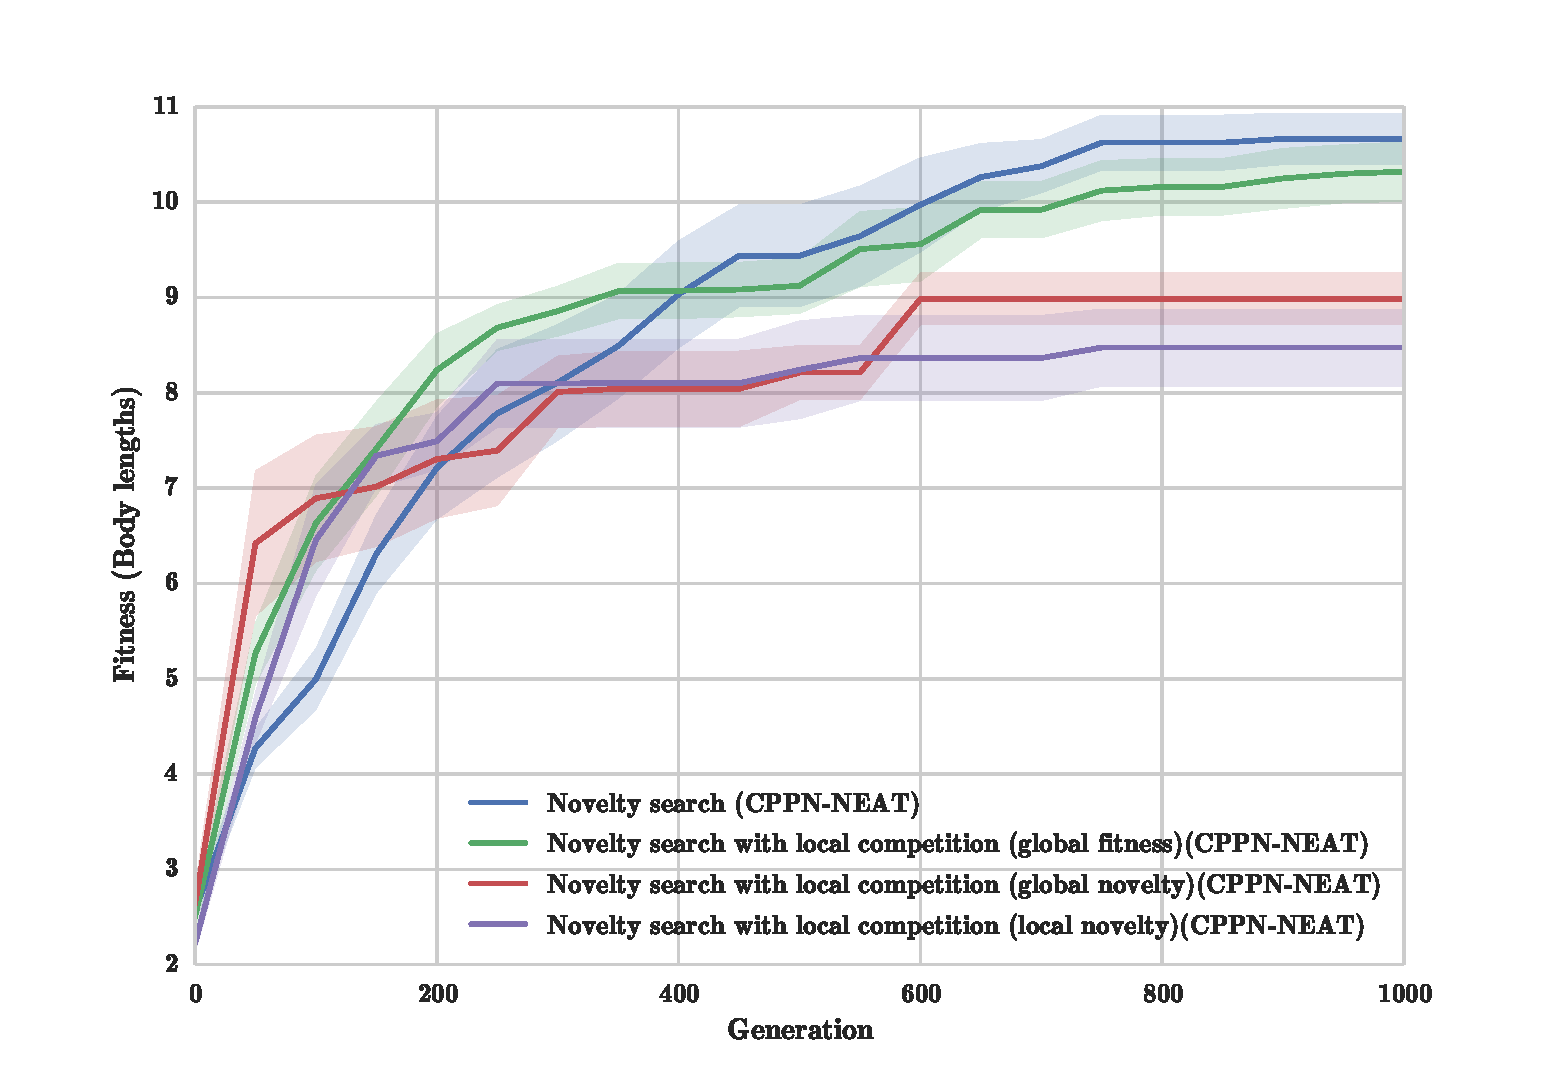
\includegraphics[width=1.0\textwidth]{../Figures/Results/NoveltyCompetitionsSize5.pdf}
\caption{Best so far fitness averaged over $10$ runs, for local competition held among the population of each species for \emph{novelty} search with generative encoding. (Settings~\ref{Settings-size5})}
\label{fig:NoveltyCompetitionsSize5}
\end{figure}


\subsubsection*{\emph{Fitness} Search}

To discuss the effects of the selection method used in the specific evolutionary setting, a second selection technique used in both fitness-based and novelty search. Figure~\ref{fig:fitComp100_20percent}, presents the results for two different selection methods, random selection from the top $20\%$ (\textcolor{MidnightBlue}{Blue}) of the population and competition among individuals from the whole part of the current population (\textcolor{BrickRed}{Red}). The size of the competition used in this experiment was $4$, meaning that the best solution in respect to its fitness value from $4$-random picks would be chosen to breed, for every generated solution. Since, NEAT (see Sec.~\ref{NEAT}) method uses speciation, the competition is held among each species. As expected, competition and the fact that the whole population has the opportunity to breed, contribute to the diversity of the population. This can be easily seen in this figure, random selection within the top $20\%$ of the population does not allow solutions to reproduce meaning that it does not explore weaker individuals, which may have the potential to become better after a decent number of mutations or cross-overs with other individuals. The deviation of the first method gives a perfect clue about how narrow is the fitness landscape at the converged area of search when only the best solutions of each generation are surviving.

\subsubsection*{\emph{Novelty} Search}

Since the algorithmic framework is the same for both search methods, competition can also be applied in novelty search. Figure~\ref{fig:NoveltyCompetitionsSize5}, presents the results when competition is held among individuals of the whole generation's population within the same species. Competition is held among individuals in respect to their global (when they are compared to all novel solutions) and local (when they are only compared to their species' population of novel behaviors) novelty, \textcolor{BrickRed}{red}, and \textcolor{Purple}{purple} lines respectively. In both cases, the overall performance of the evolution averaged on $10$ runs is worse than pure novelty search method, where individuals are selected randomly from the top-$20\%$ of the population. Both selection methods, set aside a gain early in the evolution, are performing poorly set side by side with the default selection method. Selecting individuals with high novelty within the species is crucial for the performance, since these individuals can have low novel value when compared with the global population, leading to steps backwards in the evolution towards highly novel individuals. On the other hand, when individuals are competing using their global novelty measure leads to a slightly better performance, still far from the default setting. In the contrary to the fitness-based method where competition achieved an improvement, competition within novelty search was not successful. 

Competition allows individuals to breed although they are not in the top part of the population in respect to a measure. For fitness-based search this means that soft-robots with low displacement will be allowed to breed and some of them eventually become better. For novelty search, behaviors with low novelty (behaviors located in a dense area of observed behaviors) is less probable that they will contribute in generating novel behaviors in future generations. Hence, allowing low novelty solutions to survive harms the performance of novelty search.


\section{Incorporate \emph{fitness} Information into \emph{Novelty} Search}

The reason that novelty search is considered such an revolutionary search method is because it finds solutions for deceptive problems, where the fitness landscape is not a straightforward function. What makes it so unique, it is the fact that instead of looking for optimizing the solutions in respect to an objective function is looking for the novelty in the behavior space. On each generation of novelty search novel behaviors that are also fit in regards to the objective of the problem are discovered. Mutations of these solutions will yield in behaving similarly to their ancestors, resulting in similar behaviors. Thus, the novelty value of these individuals will be declined as similar behaviors will contribute in a denser area in the behavior space. Eventually these solutions will stop being selected, and evolution will not have the change of carrying their valuable genes along. Mutations and other genetic operations can optimize these fit individuals more. These individuals (with high fitness value) can be seen as \emph{stepping~stones}~\citep{lehman2011abandoning} towards more optimized versions of them. Being blind to the objective function, novelty search will eventually stop producing new individuals out of them, which will lead to promising individuals being unable to survive through the evolution process.

\subsection*{Fitness-Competition in Novelty Search}


Competition is a simple way of combining these two search methods together. In this experiment, the number of new individuals each species will breed is determined by the average novelty value of each species. Competition is selecting these individuals not in respect to their novelty but regarding their fitness value. Elitism also copies the most novel behavior that observed within each species to the next generation. After each generation is produced, competition is held over all the population within each species to select individuals for reproduction. Figure~\ref{fig:NoveltyCompetitionsSize5}, illustrates the results of using the fitness of an individual as a measure for selection among two generations. The resulted best so far fitness (\textcolor{ForestGreen}{Green} line), reveals that competition for fitness in a novelty search setting disturbs the balance of the evolution towards novelty, not allowing novelty search to expand the search in the behavior space in a greater extend, since it is not the case that selected fit individuals will lead in novel behaviors. 

\subsection*{Fitness-Elitism in Novelty Search}

\begin{figure}[t!]
\centering
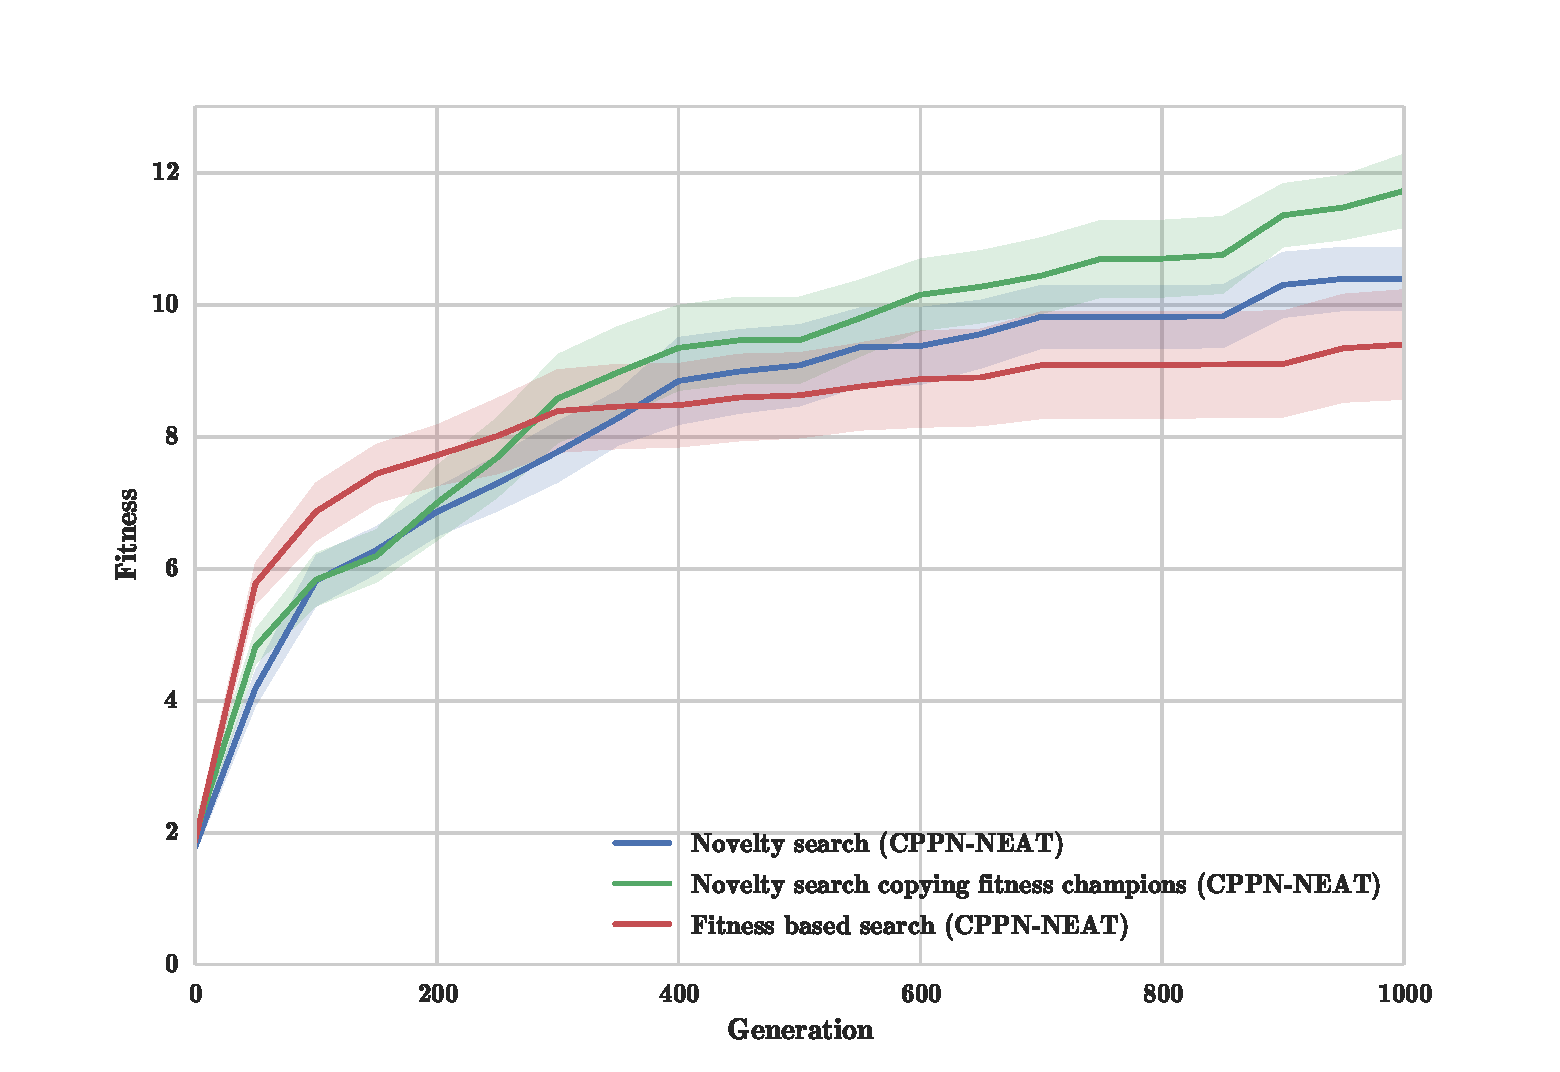
\includegraphics[width=1.0\textwidth]{../Figures/Results/CopyFitChampions10.pdf}
\caption{Best so far fitness averaged over $10$ runs, for \emph{novelty} search with and without copying \emph{fit} champions and \emph{fitness} search. (Settings~\ref{Settings-size10})}
\label{fig:CopyFitChampions10}
\end{figure}

It has been shown, how selecting individuals in respect to their fitness by competition leads to a declined performance for novelty search. Hence, an approach is proposed for incorporating fitness information into novelty search without perturbing with its pipeline. Elitism is the process of passing mutations or copies of the best individuals to the next generation. In this way best individuals are preserved and can be optimized later. The best individuals of each species generation are protected so they can contribute with their beneficial genes later in the evolution. Novelty search can include elitism in its selection process, and it does that by copying the most novel organisms of the current population of each species to the next. Since, there is no point of changing this function, elitism can be used also to copy fit individuals within novelty search method. The way these two elitism functions can be combined together depends on the population size, and the problem, while probabilistic methods can also be used. In the specific setting, both elitism function copy new individuals to the new generation. Moreover, evolution towards novelty does not get disturbed, at the same time, fit individuals have the chance to be optimized further as long as they are the fittest within the species population. Figure~\ref{fig:CopyFitChampions10}, illustrates the gain in performance when fitness elitism is used in novelty search method compared with the pure novelty and fitness-based search methods.



In this section two ways of incorporating fitness information into novelty search method discussed. Competition and elitism can be used within the pipeline of novelty search in an evolutionary algorithm to use fitness information of individuals. The latter achieved to an improvement over pure novelty search method.















\section{Evolving Soft-Robots for Outer Space}  

\begin{figure}[t!]
\centering
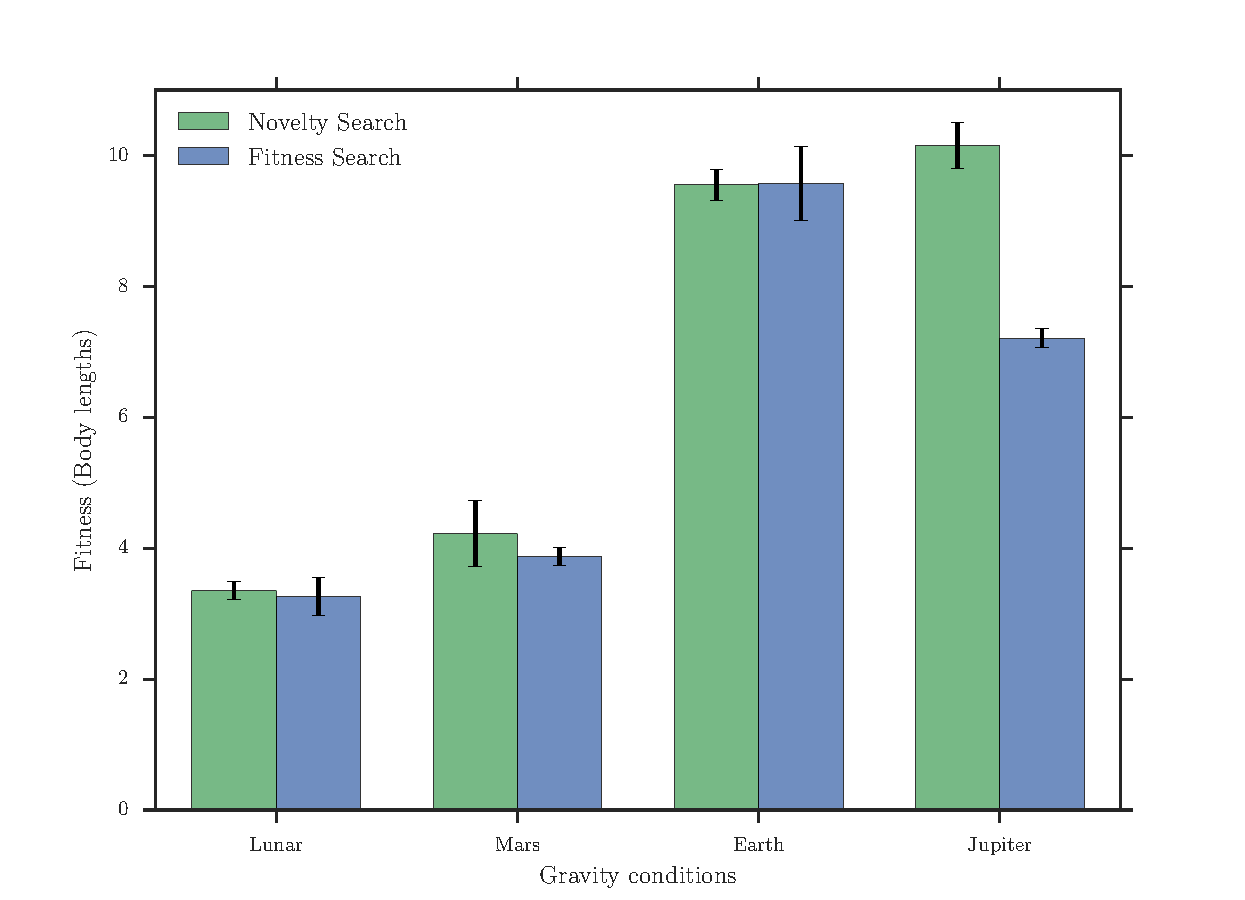
\includegraphics[width=0.8\textwidth]{../Figures/Results/GravityExperiment.pdf}
\caption{Novelty search performs equally good or better than fitness based search in all gravity conditions tested. (Settings~\ref{gravitySettings})}
\label{fig:gravityConditions}
\end{figure}

In this section, it is of interest to show how different environmental conditions can affect both the performance and the type of locomotion produced by the evolved soft robots. Both search methods discussed in this thesis, novelty and fitness-based search are used for the co-evolution of the morphology and the locomotion strategy of soft-robots under variant gravity levels. Since the software used for the simulation of the soft-robots cannot reproduce the conditions of other planets/moons in our solar system, the gravity acceleration of the environment is the only altered variable of the simulation environment. For the novelty search method two dimensional trajectories of the soft bodies are chosen as the behavior metric to evaluate the novelty of each individual. Due to the computationally expensive simulation for structures of resolution $10^3$, the performance of the locomotion strategies evolved is measured in a smaller lattice resolution $7^3$ ($10$-runs for each gravity level for both methods). Settings used in all previous experiments, were also used for Jupiter's and Earth's gravity accelerations, the simulation time used for both was $0.4$ seconds. For Lunar's and Mars' evolution runs, a higher temperature period was used ($0.050$ instead of $0.025$ seconds), in order effective locomotion to take place. High frequencies tend not to allow soft-body structures produce any decent locomotion in lower gravity conditions. Furthermore, for the lower gravity of Lunar and Mars, the simulation time was increased up to $1$ second for each evaluation. However, the final displacement of the robots was normalized to meet the expected displacement for $0.4$ seconds (the displacement of soft-robots is roughly linear to time).

Figure~\ref{fig:gravityConditions}, illustrates the performance of novelty and fitness-based search, in four different gravity conditions for Lunar ($-1.6~m/s^2$), Mars ($-3.7~m/s^2$), Earth ($-9.7~m/s^2$), and Jupiter ($-24.8~m/s^2$). The best fitness achieved by an individual averaged for all runs are shown, together with the deviation errors. Novelty search achieves in producing better or equally good locomotion for the soft-robots evolved in all gravity conditions. The results on different settings verify that novelty search can indeed achieve higher performance in the specific problem task. 

The rest of this section discusses in detail findings during the experiment in regards to the evolved locomotion strategies and morphologies capable to produce efficient locomotion. Although the measured performance of $10$ evolution runs can give us a clear estimate of what each method can achieve in respect to the expected displacement of soft-robots, the resolution of $7^3$ is not high enough to unveil complex morphologies. Three runs of both evolutionary methods in a higher resolution ($10^3$) lattice cannot give an approximation about the performance achieved by the soft-robots evolved, whilst evolved morphologies and locomotion strategies can be investigated.



\begin{figure}[t!]
\centering
\begin{subfigure}[b]{1.0\textwidth}
\foreach \i in {1,2,3,4,5,6,7}{ 
\includegraphics[width=0.132\textwidth]{../Figures/Robots/fit-g1-1-\i.jpg}
}
\caption{3-legged hopper (Fitness-Search)}
\label{fig:gravityRobots1.6-1}
\end{subfigure}
\begin{subfigure}[b]{1.0\textwidth}
\foreach \i in {1,2,3,4,5,6,7}{ 
\includegraphics[width=0.132\textwidth]{../Figures/Robots/fit-g1-2-\i.jpg}
}
\caption{Triangle shaped hopper (Fitness-Search)}
\label{fig:gravityRobots1.6-2}
\end{subfigure}
\begin{subfigure}[b]{1.0\textwidth}
\foreach \i in {1,2,3,4,5,6,7}{ 
\includegraphics[width=0.132\textwidth]{../Figures/Robots/nov-g1-1-\i.jpg}
}
\caption{L-shaped hopper (Novelty-Search)}
\label{fig:gravityRobots1.6-3}
\end{subfigure}
\begin{subfigure}[b]{1.0\textwidth}
\foreach \i in {2,3,4,5,6,8,9}{ 
\includegraphics[width=0.132\textwidth]{../Figures/Robots/nov-g1-2-\i.jpg}
}
\caption{C-shaped hopper (Novelty-Search)}
\label{fig:gravityRobots1.6-4}
\end{subfigure}
\caption{\textbf{Lunar}: Locomotion strategies evolved in low-gravity conditions consist mostly of hopper soft-robots. (Settings~\ref{Settings-size10-moon})}
\label{fig:gravityRobots1.6}
\end{figure}

\subsection{Soft-Robots on Lunar}

Locomotion strategies evolved under low gravity conditions, for the gravity of the Lunar more specifically, showed that hopping behaviors can only produce effective locomotion in these conditions. Low gravity makes it difficult for the soft-body structures to grip on the ground surface and evolve something different than hopping. Figure~\ref{fig:gravityRobots1.6}, shows four different types of hopper soft-robots under Lunar's gravity. However, the morphology of each hopper differs. A 3-legged hopper (see Fig.~\ref{fig:gravityRobots1.6-1}) uses its leg in the middle to hop, stabilizing itself with the help of its front and back legs. One legged hoppers can be evolved with different morphologies, a triangle shaped body (see Fig.~\ref{fig:gravityRobots1.6-2}), L-shaped (see Fig.~\ref{fig:gravityRobots1.6-3}), and a C-shaped soft-robot (see Fig.~\ref{fig:gravityRobots1.6-2}). Hopper soft-robots are difficult to develop a stable locomotion strategy, since most of the times the hopping technique they use is failing after few simulation seconds. Moreover, stable locomotion is difficult to be evolved, since the evolution objective is the locomotion speed. 









\begin{figure}[t!]
\centering
\begin{subfigure}[b]{1.0\textwidth}
\foreach \i in {1,3,5,6,7,8,10}{ 
\includegraphics[width=0.132\textwidth]{../Figures/Robots/fit-g3-1-\i.jpg}
}
\caption{2-legged galloping (Fitness-Search)}
\label{fig:gravityRobots3.7-1}
\end{subfigure}
\begin{subfigure}[b]{1.0\textwidth}
\foreach \i in {1,2,3,4,5,7,8}{ 
\includegraphics[width=0.132\textwidth]{../Figures/Robots/nov-g3-1-\i.jpg}
}
\caption{2-legged C-shaped hopper (Novelty-Search)}
\label{fig:gravityRobots3.7-2}
\end{subfigure}
\caption{\textbf{Mars}: Gravity acceleration on Mars allows both galloping and hopping locomotion strategies. (Settings~\ref{Settings-size10-mars})}
\label{fig:gravityRobots3.7}
\end{figure}

\subsection{Soft-Robots on Mars}

The locomotion effectiveness on Mars was higher when compared to this on Moon's gravity acceleration, making it possible for the virtual soft-robots to develop other kinds of gaits using legs. Figure~\ref{fig:gravityRobots3.7}, presents two evolved virtual creatures, where the one is galloping having a two-legged body (see Fig.~\ref{fig:gravityRobots3.7-1}), and the next is hopping having a C-shaped soft-body (see Fig.~\ref{fig:gravityRobots3.7-2}). Note that the C-shaped hopper soft-robot mostly uses passive materials apart from its upper body, where all the active material are located. With using its upper part generates enough motion able to move itself. What was observed in the soft-robots evolved in lower gravity levels was the fact that morphologies with less active voxels can produce decent locomotion.


\begin{figure}[t!]
\centering
\begin{subfigure}[b]{1.0\textwidth}
\foreach \i in {1,2,3,4,5,6,7,8,9,10}{ 
\includegraphics[width=0.088\textwidth]{../Figures/Robots/fit-g9-1-\i.jpg}
}
\caption{Top view, 2-legged galloping (Fitness-Search)}
\label{fig:gravityRobots9.8-1}
\end{subfigure}
\begin{subfigure}[b]{1.0\textwidth}
\foreach \i in {1,2,3,4,5,6,7,8,9,10}{ 
\includegraphics[width=0.088\textwidth]{../Figures/Robots/fit-g9-2-\i.jpg}
}
\caption{Top view, 4-legged animal like locomotion (Fitness-Search)}
\label{fig:gravityRobots9.8-2}
\end{subfigure}
\begin{subfigure}[b]{1.0\textwidth}
\foreach \i in {1,2,3,4,5,7,8}{ 
\includegraphics[width=0.13\textwidth]{../Figures/Robots/nov-g9-1-\i.jpg}
}
\caption{Tumbleweed-like locomotion (Novelty-Search)}
\label{fig:gravityRobots9.8-3}
\end{subfigure}
\caption{\textbf{Earth}: Morphologies evolved in gravity conditions on Earth, show that life-like locomotion strategies can be generated by soft-body creatures in a simulated environment. (Settings~\ref{Settings-size10-earth})}
\label{fig:gravityRobots9.8}
\end{figure}

\subsection{Soft-Robots on Earth}

On higher gravity levels, life-like locomotion emerges. Figure~\ref{fig:gravityRobots9.8}, shows three different locomotion strategies generated by fitness-based and novelty search on gravity conditions of Earth. Galloping-type locomotion is again observed by evolved two-legged shaped body creatures (see Fig.~\ref{fig:gravityRobots9.8-1}). Interesting animal-like gait has also been evolved (see Fig.~\ref{fig:gravityRobots9.8-2}), verifying the connection there is between gravity and the locomotion strategies of living organisms evolving on Earth for thousands of years. Tumbleweed-like locomotion (see Fig.~\ref{fig:gravityRobots9.8-3}) has been emerged under novelty search method, producing rolling soft-robots that can locomote efficiently. Fact that adds significance to the novelty-search method, since fitness-based search did not produce this kind of locomotion strategy. Tumbleweed is a concept of low-cost exploration that has inspired robot designers for Mars' missions in the past~\citep{antol2003low}, and has been already deployed in Antarctica for testing purposes by NASA.



\subsection{Soft-Robots on Jupiter}

Moving on to higher gravity levels, Jupiter, heavier structures can use galloping as a strategy for their locomotion. Figure~\ref{fig:gravityRobots27.6}, presents some of the locomotion types when novelty and fitness-based search were used for the evolution of them. Galloping (see Fig.~\ref{fig:gravityRobots27.6-1}) is again considered to be an effective way of moving in such a high gravity, whereas thicker legs are evolved to withstand the high gravitational force. Push-pull worm-like locomotion (see Fig.~\ref{fig:gravityRobots27.6-2}), can also produce decent velocities to soft-robots. Finally, hoppers have also been evolved to this setting, while they are using more actuated materials.


Different locomotion strategies can be evolved on different gravity levels producing effective locomotion. Low gravity does not allow other kinds of locomotion apart from hoppers to be evolved, while higher gravity acceleration allows more complicated behaviors to be evolved. In all settings, both search methods produced effective locomotion for the soft-body structures, however, the performance in regard to the objective measure defined, displacement of the body in body lengths, was equal or higher for novelty search in all gravity settings.


\begin{figure}[t!]
\centering
\begin{subfigure}[b]{1.0\textwidth}
\foreach \i in {1,2,3,4,5,7,8}{ 
\includegraphics[width=0.132\textwidth]{../Figures/Robots/fit-g2-1-\i.jpg}
}
\caption{2-legged walking (Fitness-Search)}
\label{fig:gravityRobots27.6-1}
\end{subfigure}
\begin{subfigure}[b]{1.0\textwidth}
\foreach \i in {1,2,3,4,5,7,8}{ 
\includegraphics[width=0.132\textwidth]{../Figures/Robots/fit-g2-2-\i.jpg}
}
\caption{Push-pull locomotion (Fitness-Search)}
\label{fig:gravityRobots27.6-2}
\end{subfigure}
\begin{subfigure}[b]{1.0\textwidth}
\foreach \i in {1,2,3,7,8,9,10}{ 
\includegraphics[width=0.132\textwidth]{../Figures/Robots/nov-g2-1-\i.jpg}
}
\caption{C-shaped hopper (Novelty-Search)}
\label{fig:gravityRobots27.6-3}
\end{subfigure}
\caption{\textbf{Jupiter}: Heavier structures on Jupiter's gravity level can locomote efficiently using several strategies. (Settings~\ref{Settings-size10-jupiter})}
\label{fig:gravityRobots27.6}
\end{figure}



